\documentclass[12pt]{book}

\newcommand{\thetitle}{Think Java: How to Think Like a Computer Scientist}
\title{\thetitle}

\newcommand{\theauthors}{Allen Downey and Chris Mayfield}
\author{\theauthors}

\newcommand{\theversion}{Version 6.0 Draft -- \today}
\date{\theversion}

\usepackage{geometry}
\geometry{
    width=5.5in,
    height=8.5in,
    hmarginratio=3:2,
    vmarginratio=1:1,
    includehead=true,
    headheight=15pt
}

% paragraph spacing
\setlength{\parindent}{0pt}                      % 17.62482pt
\setlength{\parskip}{12pt plus 4pt minus 4pt}    % 0.0pt plus 1.0pt
\linespread{1.05}
\def\arraystretch{1.5}

% list spacing
\setlength{\topsep}{5pt plus 2pt minus 3pt}      % 10.0pt plus 4.0pt minus 6.0pt
\setlength{\partopsep}{-6pt plus 2pt minus 2pt}  %  3.0pt plus 2.0pt minus 2.0pt
\setlength{\itemsep}{0pt}                        %  5.0pt plus 2.5pt minus 1.0pt

% these are copied from tex/latex/base/book.cls
% all I changed is afterskip
\makeatletter
\renewcommand{\section}{\@startsection {section}{1}{\z@}%
    {-3.5ex \@plus -1ex \@minus -.2ex}%
    {0.7ex \@plus.2ex}%
    {\normalfont\Large\bfseries}}
\renewcommand\subsection{\@startsection{subsection}{2}{\z@}%
    {-3.25ex\@plus -1ex \@minus -.2ex}%
    {0.3ex \@plus .2ex}%
    {\normalfont\large\bfseries}}
\renewcommand\subsubsection{\@startsection{subsubsection}{3}{\z@}%
    {-3.25ex\@plus -1ex \@minus -.2ex}%
    {0.3ex \@plus .2ex}%
    {\normalfont\normalsize\bfseries}}
\makeatother

% table of contents vertical spacing
\usepackage{tocloft}
\setlength\cftparskip{8pt plus 4pt minus 4pt}

% The following line adds a little extra space to the column
% in which the Section numbers appear in the table of contents
\makeatletter
\renewcommand{\l@section}{\@dottedtocline{1}{1.5em}{3.0em}}
\makeatother

% customize page headers
\usepackage{fancyhdr}
\pagestyle{fancyplain}
\renewcommand{\chaptermark}[1]{\markboth{Chapter \thechapter ~~ #1}{}}
\renewcommand{\sectionmark}[1]{\markright{\thesection ~~ #1}}
\lhead[\fancyplain{}{\bfseries\thepage}]%
      {\fancyplain{}{\bfseries\rightmark}}
\rhead[\fancyplain{}{\bfseries\leftmark}]%
      {\fancyplain{}{\bfseries\thepage}}
\cfoot{}
%\rfoot{\textcolor{gray}{\tiny ThinkJava Draft \today}}

% balanced index with TOC entry
\usepackage{makeidx}
\makeindex
%\usepackage[totoc]{idxlayout}

% automatically index glossary terms
\newcommand{\term}[1]{%
\index{#1}
\item[#1:]}
% TODO: doesn't work with plastex
%\newcommand{\term}[1]{\item[#1:]}

% where to find graphics
\usepackage{graphicx}
%\graphicspath{{figs/}}

%% tweak spacing of figures and captions
%\usepackage{floatrow}
%\usepackage{caption}
%\captionsetup{
%    font=small,
%    labelformat=empty,
%    justification=centering,
%    skip=4pt
%}

% format end of chapter excercises
\usepackage{amsmath}
\usepackage{amsthm}
\newtheoremstyle{exercise}
  {12pt}        % space above
  {12pt}        % space below
  {}            % body font
  {}            % indent amount
  {\bfseries}   % head font
  {}            % punctuation
  {12pt}        % head space
  {}            % custom head
\theoremstyle{exercise}
\newtheorem{exercise}{Exercise}[chapter]

% colors for code listings and output
\usepackage{xcolor}
\definecolor{bgcolor}{HTML}{FAFAFA}
\definecolor{comment}{HTML}{007C00}
\definecolor{keyword}{HTML}{0000FF}
\definecolor{strings}{HTML}{B20000}

% syntax highlighting in code listings
\usepackage{textcomp}
\usepackage{listings}
\lstset{
    language=java,
    basicstyle=\ttfamily,
    backgroundcolor=\color{bgcolor},
    commentstyle=\color{comment},
    keywordstyle=\color{keyword},
    stringstyle=\color{strings},
    columns=fullflexible,
    keepspaces=true,
    showstringspaces=false,
    upquote=true,
    aboveskip=\parskip,
    belowskip=\parskip
}

% code listing environments
\lstnewenvironment{code}
{\minipage{\linewidth}}
{\endminipage}
\lstnewenvironment{stdout}
{\lstset{commentstyle=,keywordstyle=,stringstyle=}\minipage{\linewidth}}
{\endminipage}

% pdf hyperlinks, table of contents, and document properties
\usepackage[pdftex]{hyperref}
\hypersetup{%
  pdftitle={\thetitle},
  pdfauthor={\theauthors},
  pdfsubject={\theversion},
  pdfkeywords={},
  bookmarksopen=false,
  colorlinks=true,
  citecolor=black,
  filecolor=black,
  linkcolor=black,
  urlcolor=blue
}

% inline syntax formatting
\newcommand{\java}[1]{\lstinline{#1}} %\end{
%\newcommand{\java}[1]{\verb"#1"}
%\newcommand{\java}[1]{{\tt #1}}

\begin{document}

\frontmatter

%-half title--------------------------------------------------
%\thispagestyle{empty}
%
%\begin{flushright}
%\vspace*{2.0in}
%
%{\huge Think Java}
%
%\vspace{0.25in}
%{\LARGE How to Think Like a Computer Scientist}
%
%\vfill
%
%\end{flushright}

%--verso------------------------------------------------------

%\cleardoublepage
%\cleardoublepage

%--title page--------------------------------------------------
\pagebreak
\thispagestyle{empty}

\begin{flushright}
\vspace*{2.0in}

{\huge Think Java}

\vspace{0.25in}
{\LARGE How to Think Like a Computer Scientist}

\vspace{1in}
{\Large \theauthors}

\vspace{1in}
{\large \theversion}

\vfill

\end{flushright}

%--copyright--------------------------------------------------
\pagebreak
\thispagestyle{empty}

Copyright \copyright ~2016 Allen Downey and Chris Mayfield.

{\bf NOTE: This version of the book is a work in progress and won't be completed until February 2016.}

\vspace{0.25in}

Permission is granted to copy, distribute, transmit, and adapt this work under the Creative Commons Attribution-NonCommercial-ShareAlike 3.0 Unported License: \url{http://creativecommons.org/licenses/by-nc-sa/3.0/}

The original form of this book is \LaTeX\ source code.
Compiling the \LaTeX\ source has the effect of generating a device-independent representation of the book, which can be converted to other formats and printed.

The \LaTeX\ source for this book is available from \url{http://thinkjava.org}.
%-----------------------------------------------------------------

%\chapter{Preface}

\begin{quote}
``As we enjoy great Advantages from the Inventions of others,
we should be glad of an Opportunity to serve others by any
Invention of ours, and this we should do freely and generously.''

---Benjamin Franklin, quoted in {\em Benjamin Franklin} by
Edmund S. Morgan.
\end{quote}

\subsection*{Why I wrote this book}

This is the fifth edition of a book I started writing in 1999,
when I was teaching at Colby College.  I had taught an introductory
computer science class using the Java programming language, but I
had not found a textbook I was happy with.  For one thing,
they were all too big!  There was no way my students would read
800 pages of dense, technical material, even if I wanted them to.
And I didn't want them to.  Most of the material was too
specific---details about Java and its libraries that would be obsolete
by the end of the semester, and that obscured the material I really
wanted to get to.

The other problem I found was that the introduction to object-oriented
programming was too abrupt.  Many students who were otherwise
doing well just hit a wall when we got to objects, whether we did
it at the beginning, middle or end.

So I started writing.  I wrote a chapter a day for 13 days, and on
the 14th day I edited.  Then I sent it to be photocopied and bound.
When I handed it out on the first day of class, I told the students
that they would be expected to read one chapter a week.  In other
words, they would read it seven times slower than I wrote it.


\subsection*{The philosophy behind it}

Here are some of the ideas that make the book the way it is:

\begin{itemize}

\item Vocabulary is important.  Students need to be able to talk
about programs and understand what I am saying.  I try to
introduce the minimum number of terms, to define them carefully
when they are first used, and to organize them in glossaries
at the end of each chapter.  In my class, I include vocabulary
questions on quizzes and exams, and require students to use
appropriate terms in short-answer responses.

\item To write a program, students have to understand the
algorithm, know the programming language, and they have to be
able to debug.  I think too many books neglect debugging.  This
book includes an appendix on debugging and an appendix on program
development (which can help avoid debugging).  I recommend that
students read this material early and come back to it often.

\item Some concepts take time to sink in.  Some of the more
difficult ideas in the book, like recursion, appear several times.
By coming back to these ideas, I am trying to give students a
chance to review and reinforce or, if they missed it the first time,
a chance to catch up.

\item I try to use the minimum amount of Java to get the
maximum amount of programming power.  The purpose of this book
is to teach programming and some introductory ideas from computer
science, not Java.  I left out some language features, like
the {\tt switch} statement, that are unnecessary, and avoided
most of the libraries, especially the ones like the AWT that have been
changing quickly or are likely to be replaced.

\end{itemize}

The minimalism of my approach has some advantages.
Each chapter is about ten pages, not including the exercises.
In my classes I ask students to read each chapter before we
discuss it, and I have found that they are willing to do that
and their comprehension is good.  Their preparation makes
class time available for discussion of the more abstract material,
in-class exercises, and additional topics that aren't in the
book.

But minimalism has some disadvantages.  There is not much here
that is intrinsically fun.  Most of my examples demonstrate the
most basic use of a language feature, and many of the exercises
involve string manipulation and mathematical ideas.  I think some
of them are fun, but many of the things that excite students
about computer science, like graphics, sound and network applications,
are given short shrift.

The problem is that many of the more exciting features involve
lots of details and not much concept.  Pedagogically, that means
a lot of effort for not much payoff.  So there is a tradeoff between
the material that students enjoy and the material that is most
intellectually rich.  I leave it to individual teachers to find
the balance that is best for their classes.  To help, the book
includes appendices that cover graphics, keyboard input and
file input.

\subsection*{Object-oriented programming}

Some books introduce objects immediately; others warm up with a more
procedural style and develop object-oriented style more gradually.
This book uses the ``objects late'' approach.

Many of Java's object-oriented features are motivated
by problems with previous languages, and their implementations
are influenced by this history.  Some of these features are
hard to explain if students aren't familiar with the problems
they solve.

It wasn't my intention to postpone object-oriented programming.
On the contrary, I got to it as quickly as I could, limited by
my intention to introduce concepts one at a time, as clearly
as possible, in a way that allows students to practice each
idea in isolation before adding the next.  But I have to admit
that it takes some time to get there.

\subsection*{The Computer Science AP Exam}

Naturally, when the College Board announced that the AP Exam
would switch to Java, I made plans to update the Java version of
the book.  Looking at the proposed AP Syllabus, I saw that their
subset of Java was all but identical to the subset I had chosen.

During January 2003, I worked on the Fourth Edition of the book,
making these changes:

\begin{itemize}

\item I added sections to improve coverage of the AP syllabus.

\item I improved the appendices on debugging and program development.

\item I collected the exercises, quizzes, and exam questions I
had used in my classes and put them at the end of the appropriate
chapters.  I also made up some problems that are intended to
help with AP Exam preparation.

\end{itemize}

Finally, in August 2011 I wrote the fifth edition, adding
coverage of the GridWorld Case Study that is part of the AP Exam.


\subsection*{Free books!}

Since the beginning, this book has been under a license that allows users
to copy, distribute and modify the book.  Readers can download the
book in a variety of formats and read it on screen or print it.
Teachers are free to print as many copies as they need.  And anyone is
free to customize the book for their needs.

People have translated the book into other computer languages
(including Python and Eiffel), and other natural languages (including
Spanish, French and German).  Many of these derivatives are also
available under free licenses.

Motivated by Open
Source Software, I adopted the philosophy of releasing the
book early and updating it often.  I do my best to minimize the
number of errors, but I also depend on readers to help out.

The response has been great.  I get messages almost every day from
people who have read the book and liked it enough to take the trouble
to send in a ``bug report.''  Often I can correct an error
and post an updated version within a few minutes.  I think of the
book as a work in progress, improving a little whenever I have time
to make a revision, or when readers send feedback.

\subsection*{Oh, the title}

I get a lot of grief about the title of the book.  Not everyone
understands that it is---mostly---a joke.
Reading this book will probably not make you think like a computer
scientist.  That takes time, experience, and probably a few more
classes.

But there is a kernel of truth in the title: this book is not
about Java, and it is only partly about programming.  If it is
successful, this book is about a way of thinking.  Computer scientists
have an approach to problem-solving, and a way of crafting solutions,
that is unique, versatile and powerful.  I hope that this book
gives you a sense of what that approach is, and that at some
point you will find yourself thinking like a computer scientist.

\vspace{0.2in}

\begin{flushleft}
Allen Downey\\
Needham, Massachusetts\\
July 13, 2011
\end{flushleft}


\section*{Contributors List}

When I started writing free books, it didn't occur to me to keep
a contributors list.  When Jeff Elkner suggested it, it seemed so
obvious that I am embarassed by the omission.  This list starts
with the 4th Edition, so it omits many people who contributed
suggestions and corrections to earlier versions.

If you have additional comments, please send them to: \\
\href{mailto:feedback@greenteapress.com}{feedback@greenteapress.com}

\begin{itemize}

\item Ellen Hildreth used this book to teach Data Structures at
Wellesley College, and she gave me a whole stack of corrections,
along with some great suggestions.

\item Tania Passfield pointed out that the glossary of Chapter 4
has some leftover terms that no longer appear in the text.

\item Elizabeth Wiethoff noticed that my series expansion of
$\exp(-x^2)$ was wrong.  She is also working on a Ruby version of
the book!

\item Matt Crawford sent in a whole patch file full of corrections!

\item Chi-Yu Li pointed out a typo and an error in one of the code
examples.

\item Doan Thanh Nam corrected an example in Chapter 3.

\item Stijn Debrouwere found a math typo.

\item Muhammad Saied translated the book into Arabic, and found
several errors.

\item Marius Margowski found an inconsistency in a code example.

\item Guy Driesen found several typos.

\item Leslie Klein discovered yet another error in the series expansion
of $\exp(-x^2)$, identified typos in the card array figures, and gave
helpful suggestions to clarify several exercises.

\end{itemize}

Finally, I wish to acknowledge Chris Mayfield for his significant
contribution to version 5.1 of this book. His careful review
lead to over one hundred corrections and improvements throughout.
Several new features include embedded hypertext links and cross
references, consistent layout of all exercises, and Java syntax
highlighting in code examples.

% endcontrib


% table of contents
\cleardoublepage
\setcounter{tocdepth}{1}
\tableofcontents

\mainmatter


\chapter{The way of the program}

The goal of this book is to teach you to think like a computer scientist.
This way of thinking combines some of the best features of mathematics, engineering, and natural science.
Like mathematicians, computer scientists use formal languages to denote ideas (specifically computations).
Like engineers, they design things, assembling components into systems and evaluating trade-offs among alternatives.
And like scientists, they observe the behavior of complex systems, form hypotheses, and test predictions.

\index{problem-solving}

The single most important skill for a computer scientist is {\bf problem-solving}.
It involves the ability to formulate problems, think creatively about solutions, and express solutions clearly and accurately.
As it turns out, the process of learning to program is an excellent opportunity to develop problem-solving skills.
That's why this chapter is called, ``The way of the program.''

On one level you will be learning to program, a useful skill by itself.
But on another level you will use programming as a means to an end.
As we go along, that end will become clearer.
Learning how to think in terms of computation is much more valuable than simply learning how to write code.


\section{What is programming?}

\index{program}

A {\bf program} is a sequence of instructions that specifies how to perform a computation.
%\footnote{This definition does not apply to all programming languages; for alternatives, see \url{http://en.wikipedia.org/wiki/Declarative_programming}.}
The computation might be something mathematical, like solving a system of equations or finding the roots of a polynomial.
It can also be a symbolic computation, like searching and replacing text in a document or (strangely enough) compiling a program.
The details look different in different languages, but a few basic instructions appear in just about every language.

\begin{description}
\item[input:] Get data from the keyboard, a file, a sensor, or some other device.
\item[output:] Display data on the screen or send data to a file or other device.
\item[math:] Perform basic mathematical operations like addition and division.
\item[decisions:] Check for certain conditions and execute the appropriate code.
\item[repetition:] Perform some action repeatedly, usually with some variation.
\end{description}

\index{programming}

Believe it or not, that's pretty much all there is to it.
Every program you've ever used, no matter how complicated, is made up of instructions that look much like these.
So you can think of {\bf programming} as the process of breaking down a large, complex task into smaller and smaller subtasks.
The process continues until the subtasks are simple enough to be performed with the basic instructions provided by computer hardware.


\section{What is computer science?}

One of the most interesting aspects of writing programs is deciding how to solve a particular problem, especially when there are multiple solutions.
For example, there are numerous ways to sort a list of numbers, and each way has its advantages (see \url{http://www.sorting-algorithms.com/}).
In order to determine which way is best for a given situation, we need techniques for describing and analyzing solutions formally.
That is where computer science comes in.

\index{computer science}
\index{algorithm}

Put simply, {\bf computer science} is the science of algorithms, including their discovery and analysis.
An {\bf algorithm} is a sequence of steps that specify exactly how to solve a problem.
Some algorithms are better than others in terms of low long they take or how much memory they use.
As you learn to develop algorithms for problems you haven't solved before, you also learn to think like a computer scientist.
%It's much more fun to discover new algorithms than to write the code for solutions that other people came up with!

\index{bug}
\index{debugging}

Designing algorithms and writing code is difficult and error-prone.
For historical reasons, programming errors are called {\bf bugs}, and the process of tracking them down and correcting them is called {\bf debugging}.
As you learn to debug your programs, you will develop new problem-solving skills.
You will need to think creatively when unexpected errors happen.

%In the old days, computer scientists had to deal with real bugs flying into their systems.
%You probably won't have that problem, but you will need to think creatively when unexpected errors happen.

%\begin{figure}[!h]
%\begin{center}
%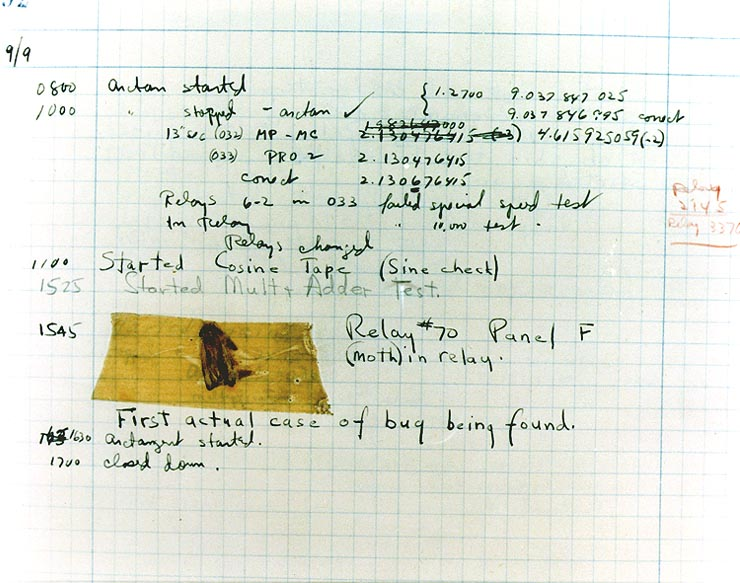
\includegraphics[height=2.2in]{figs/firstbug.jpg}
%\caption{The first computer bug, taped to Grace Hopper's log book in 1947.
%\\ She discovered the moth in an electromagnetic relay of the Mark II.}
%\end{center}
%\end{figure}

% ABD: I don't love this particular piece of mythology, partly because it's not accurate, and partly because stories about the old days bore students.

Although it can be frustrating, debugging is an intellectually rich, challenging, and interesting part of computer programming.
In some ways, debugging is like detective work.
You are confronted with clues, and you have to infer the processes and events that led to the results you see.
Thinking about how to correct programs and improve their performance sometimes even leads to the discovery of new algorithms.


\section{Introduction to Java}

\index{high-level language}
\index{language!high-level}

The programming language you will learn is Java, which is relatively new (Sun released the first version in May 1995).
Java is an example of a {\bf high-level language}.
Other high-level languages you may have heard of include C and C++, JavaScript, Python, Ruby, and Visual Basic.

\index{low-level language}
\index{language!low-level}

There are also {\bf low-level languages}, sometimes referred to as ``machine languages'' or ``assembly languages.''
Loosely speaking, computers can only run programs written in low-level languages.
So programs written in a high-level language have to be translated before they can run.
This translation takes some time, which is a small disadvantage of high-level languages.
But the advantages of high-level languages are enormous.
As a result, low-level languages are only used for programs that need to interact directly with hardware.

\index{portable}

Due to the advantages, almost all programs are written in high-level languages.
First, it is {\em much} easier to program in a high-level language.
Programs take less time to write, are shorter and easier to read, and are more likely to be correct.
Second, high-level languages are {\bf portable}, meaning that they can run on different kinds of computers with few or no modifications.
Low-level programs can only run on one kind of computer, and have to be rewritten to run on another.

\index{interpreter}

Two kinds of programs translate high-level languages into low-level languages: interpreters and compilers.
An {\bf interpreter} reads a high-level program and executes it, meaning that it does what the program says.
It processes the program a little at a time, alternately reading lines and performing computations.
% Figure 1.1 shows the structure of an interpreter.

\begin{figure}[!h]
\begin{center}
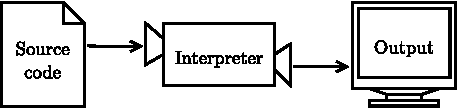
\includegraphics{figs/interpreter.pdf}
\caption{How interpreted languages like Python and Ruby are executed.}
\end{center}
\end{figure}

\index{compiler}
\index{source code}
\index{object code}
\index{executable}

In contrast, a {\bf compiler} reads the entire program and translates it completely before the program starts running.
In this context, the high-level program is called the {\bf source code}, and the translated program is called the {\bf object code} or the {\bf executable}.
Once a program is compiled, you can execute it repeatedly without further translation.
As a result, compiled programs often run faster than interpreted programs.
% Figure 1.2 shows the structure of a compiler.

\index{byte code}

Java is {\em both} compiled and interpreted.
Instead of translating programs directly into machine language, the Java compiler generates {\bf byte code}.
Similar to machine language, byte code is easy (and fast) to interpret.
But it is also portable, like a high-level language.
Thus it is possible to compile a Java program on one machine, transfer the byte code to another machine, and then execute (interpret) the byte code on the other machine.
%This ability is an advantage of Java over some other high-level languages.

\begin{figure}[!h]
\begin{center}
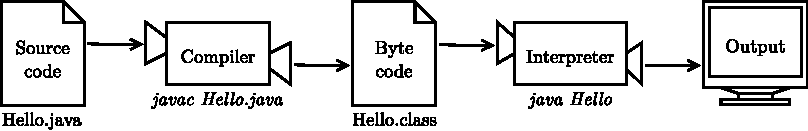
\includegraphics{figs/compiler.pdf}
\caption{The process of editing, compiling, and running a Java program.}
\end{center}
\end{figure}

Although this process may seem complicated, in most program development environments these steps are automated for you.
Usually you will only have to write a program and press a button or type a single command to compile and run it.
On the other hand, it is important to know what steps are happening in the background, so if something goes wrong you can figure out what it is.


\section{Formal languages}

\index{natural language}
\index{language!natural}

Learning a programming language is very different from learning a {\bf natural language} such as English, Spanish, or German.
The languages that people speak evolved naturally over time.
They were not designed by people, although we try to impose order on them for practical reasons.

\index{formal language}
\index{language!formal}

In contrast, {\bf formal languages} are designed by people for specific applications.
For example, the notation that mathematicians use is a formal language that is particularly good at denoting relationships among numbers and symbols.
Chemists use a formal language to represent the chemical structure of molecules.
And most importantly:

\index{programming language}
\index{language!programming}

\begin{quote}
{\bf Programming languages are formal languages that have been designed to express computations.}
\end{quote}

\index{syntax}
\index{semantics}

Formal languages have strict rules about both the {\bf syntax} (structure) and the {\bf semantics} (meaning) of statements.
For example, $3 + 3 = 6$ is a syntactically correct mathematical statement, but $3\ + = 3\ \$\ 6$ is not.
$1 + 2 = 4$ uses correct syntax, but is semantically incorrect.
$H_2O$ is a syntactically correct chemical formula, but $_2Zz$ is not.

\subsection{Tokens and grammar}

\index{token}

Syntax rules come in two flavors, pertaining to tokens and grammar.
{\bf Tokens} are the basic elements of the language, like words, numbers, and chemical elements.
One of the problems with $3\ + = 3\ \$\ 6$ is that $\$$ is not a legal token in mathematics.
Similarly, $_2Zz$ is not legal because there is no element with the abbreviation $Zz$.

\index{grammar}

The second type of syntax rule pertains to the {\bf grammar} of the language, or the way tokens can be arranged.
The statement $3\ + = 3$ is structurally illegal, even though $+$ and $=$ are legal tokens, because you can't have one right after the other.
Similarly, in a chemical formula the subscript comes after the element name, not before.

\index{parse}

When you read a sentence in English or a statement in a formal language, you have to figure out its structure.
This process is called {\bf parsing}, and in a natural language you learn to do it unconsciously.
For example, when you hear the statement ``the penny dropped,'' you understand that the penny is the subject and dropped is the predicate.
After you have parsed the statement, you can begin to figure out what it means.
%Assuming that you know what a penny is and what it means to drop, you will understand the general implication of this statement.

\subsection{Reading source code}

Although formal and natural languages have features in common---tokens, grammar, and meaning---there are some differences.

\begin{description}

\term{ambiguity}
Natural languages are full of ambiguity, which people deal with by using contextual clues and other information.
Formal languages are designed to be nearly or completely unambiguous, which means that any statement has exactly one meaning, regardless of context.

\term{redundancy}
In order to make up for ambiguity and reduce misunderstandings, natural languages employ lots of redundancy.
As a result, they are often verbose.
Formal languages are less redundant and more concise.

\term{literalness}
Natural languages are full of idiom and metaphor.
When someone says ``the penny dropped'' there is no penny and nothing dropping.
This idiom means that someone finally realized something after a period of confusion.
In contrast, formal languages mean exactly what they say.

\end{description}

People who grow up speaking a natural language---that is, everyone---often have a hard time adjusting to formal languages.
In some ways, the difference between natural and formal language is like the difference between poetry and prose, but more so.

\begin{description}

\term{poetry}
Words are used for their sounds as well as for their meaning, and the whole poem together creates an effect or emotional response.
Ambiguity is not only common but often deliberate.

\term{prose}
The literal meaning of words is more important, and the structure contributes more meaning.
Prose is more amenable to analysis than poetry but still often ambiguous.

\term{program}
The meaning of a computer program is unambiguous and literal, and can be understood entirely by analysis of the tokens and grammar.

\end{description}

%Here are some suggestions for reading programs (and other formal languages).
Remember that formal languages are much more dense than natural languages, so it takes longer to read them.
The structure is very important, so it is not always a good idea to read from top to bottom, left to right.
Over time you will learn to parse the program in your head, identifying the tokens and interpreting the structure.
Finally, the details matter.
Small errors in spelling and punctuation, which you can get away with in natural languages, can make a big difference in a formal language.


\section{The hello world program}
\label{sec:hello}

\index{hello world}

Traditionally, the first program you write when learning a new programming language is called the hello world program.
All it does is display the words ``Hello, World!''\ on the screen.
In Java, it looks like this:

\begin{code}
public class Hello {

    public static void main(String[] args) {
        // generate some simple output
        System.out.println("Hello, World!");
    }

}
\end{code}

Note the output of this program does not include the quote marks:

\begin{stdout}
Hello, World!
\end{stdout}

\index{public}
\index{static}

Unfortunately in Java, even this simple example requires language features that are difficult to explain to beginners.
But it provides a preview of topics that we will see in detail later on.
The word \java{public} means the code can be accessed from other source files.
The word \java{static} means that memory is allocated for the program in advance.
We will discuss \java{void}, \java{String}, and \java{args} in the next few chapters.
For now, let's focus on the overall structure.

\index{class!definition}
\index{method!definition}

Java programs are made up of {\bf class} and {\bf method} definitions, which generally have the form:

\begin{code}
public class CLASSNAME {

    METHOD {
        STATEMENTS
    }

    METHOD {
        STATEMENTS
    }

}
\end{code}

\index{class!name}

Here \java{CLASSNAME} indicates the name chosen by the programmer.
Java requires the class name to match the source file name.
In the hello world example, the file name must be {\tt Hello.java} because the class name is \java{Hello}.

\index{statement}
\index{main}

Classes define a program's methods, or named sequences of {\bf statements}.
The \java{Hello} class has only one method:

\begin{code}
    public static void main(String[] args)
\end{code}

The name and format of \java{main} is special; it marks the place in the class where execution begins.
When the program runs, it starts at the first statement in \java{main} and ends when it finishes the last statement.

\index{braces}
\index{squiggly braces}

Java uses squiggly braces (\{ and \}) to group things together.
In {\tt Hello.java}, the outermost braces (lines 1 and 8) contain the class definition, and the inner braces (lines 3 and 6) contain the definition of \java{main} method.

% ABD: It looks like we don't have line numbers in the listings.
% Is that a problem for the text here?

\index{println}
\index{statement!print}

The main method can have any number of statements, but the \java{Hello} example has only one.
It is a {\bf print statement}, meaning that it displays a message on the screen.
Confusingly, print can mean both ``display something on the screen'' and ``send something to the printer.''
%I won't say much about sending things to the printer;
In this book, we'll do all our printing on the screen.
The print statement ends with a semicolon ({\tt ;}).

\index{comments!inline}
\index{statement!comment}

Line 4 contains a {\bf comment}, or a bit of English text that explains the code that follows.
When the compiler sees {\tt //}, it ignores everything from there until the end of the line.
It is a good idea to write a comment before every major block of code so that other programmers (including your future self) can understand what you meant to do.


\section{Getting started with DrJava}

\index{JDK}

In order to compile Java programs on your own computer, you will need to install the Java Development Kit (JDK).
This free software by Oracle includes tools for developing and debugging Java programs.
All the examples in this book were developed and tested using Java SE Version 7.
Later versions of Java are generally backward compatible, so if you are using a more recent version, the examples in this book should still work.

\begin{figure}[!h]
\begin{center}
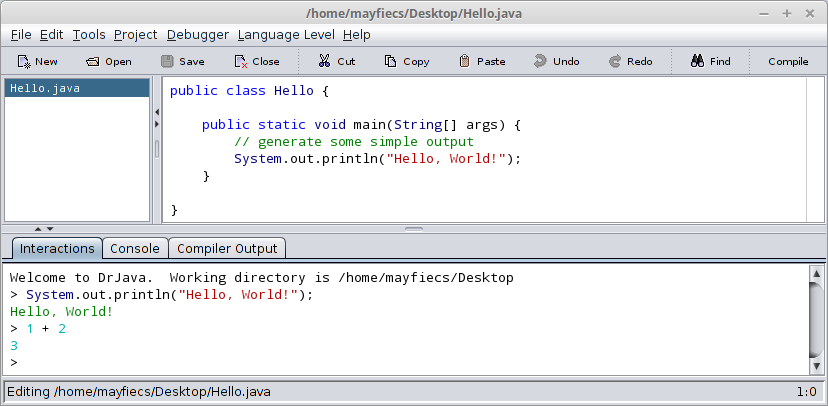
\includegraphics[width=\textwidth]{figs/drjava-hello.png}
\caption{Screenshot of DrJava editing the hello world program.}
\end{center}
\end{figure}

\index{DrJava}

We will use DrJava as the primary development environment throughout the book.
A useful feature of DrJava is the Interactions Pane at the bottom of the window.
It provides the ability to try out code quickly, without having to write a class definition and save/compile/run the program.
Refer to the DrJava documentation (\url{http://drjava.org/docs/quickstart/}) for more details.

Step-by-step instructions for installing the JDK and configuring DrJava are available on this book's website: \url{http://thinkjava.org/}

% TODO: when we have the specific URL for the install page, let's put it here.

\subsection{Command-line interface}

\index{command-line}
\index{terminal}

One of the most powerful and useful skills you can learn as a computer scientist is how to use the {\bf command-line}, also called
the {\em terminal}.
The command-line is a direct interface to the operating system.
It allows you to run programs, manage files and directories, and monitor system resources.
Many advanced tools, both for software development and general purpose computing, are available only at the command-line.

There are many good tutorials online for learning the command-line for your operating system; just search the web for ``command line tutorial.''
To get started, you only need to know four commands: how to change the working directory ({\tt cd}), list directory contents ({\tt ls}), compile Java programs ({\tt javac}), and run Java programs ({\tt java}).

% ABD: There's a conflict here between ``Find the details for your system'' and ``Here are the UNIX commands''.

\begin{figure}[!h]
\begin{center}
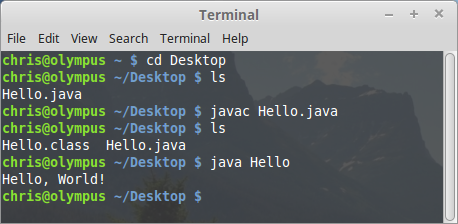
\includegraphics[width=4.5in]{figs/terminal.png}
\caption{Compiling and running {\tt Hello.java} from the command-line.}
\end{center}
\end{figure}

In this example, the {\tt Hello.java} source file is stored in the {\tt Desktop} directory.
After changing to that location and listing the files, we use the {\tt javac} command to compile {\tt Hello.java}.
Running {\tt ls} again, we see that the compiler generated a new file, {\tt Hello.class}, which contains the byte code.
We run the program using the {\tt java} command, which displays the output on the following line.

Note that the {\tt javac} command requires a {\em file name} (or multiple source files separated by spaces), whereas the {\tt java} command requires a single {\em class name}.
If you use DrJava, it runs these commands for you and displays the output in the Interactions Pane.

Taking time to learn this efficient and elegant way of interacting with your operating system will make you more productive as a computer user.
People who don't use the command-line don't know what they're missing.

% ABD: Maybe add a reference to Neal Stephenson's book?


\section{More printing}

You can put as many statements as you want in \java{main}.
For example, to print more than one line:

\begin{code}
public class Hello {

    public static void main(String[] args) {
        // generate some simple output
        System.out.println("Hello, World!");  // print one line
        System.out.println("How are you?");   // print another
    }

}
\end{code}

As this program demonstrates, you can put comments at the end of a line as well as on lines all by themselves.

\index{String}
\index{type!String}

Phrases that appear in quotation marks are called {\bf strings}, because they contain a sequence of characters strung together.
Strings can contain any combination of letters, numbers, punctuation marks, symbols, and even non-printable characters like tab and backspace.

\index{newline}
\index{print}
\index{statement!print}

The name \java{println} is short for ``print line.''
It appends a special character, called a {\bf newline}, that advances the cursor to the beginning of the next line.
%The next time \java{println} is invoked, the new text appears on the next line.
To display the output from multiple print statements on one line, use \java{print}:

\begin{code}
public class Goodbye {

    public static void main(String[] args) {
        System.out.print("Goodbye, ");
        System.out.println("cruel world");
    }

}
\end{code}

The output appears on a single line as {\tt Goodbye, cruel world}.
Notice that there is a space between the word ``Goodbye'' and the second quotation mark.
This space appears in the output, so it affects the {\em behavior} of the program.

\subsection{Code formatting}
\label{sec:formatting}

Spaces that appear outside of quotation marks generally do not affect the behavior of the program.
For example, we could have written:

\begin{code}
public class Goodbye {
public static void main(String[] args) {
System.out.print("Goodbye, ");
System.out.println("cruel world");
}
}
\end{code}

This program would compile and run just as well as the original.
The newlines at the end of each line do not affect the program's behavior either.
So we could have also written:

\begin{code}
public class Goodbye { public static void main(String[] args) {
System.out.print("Goodbye, "); System.out.println
("cruel world");}}
\end{code}

It still works, but the program is getting harder and harder to read.
Newlines and spaces are important for organizing your program visually, making it easier to understand the program and find errors when they occur.
%Formatting your code well does not take much effort, and it pays huge dividends.
%We will discuss readability and style guidelines in the next chapter.

\subsection{Escape sequences}

It is possible to print multiple lines of output in just one line of code.
You simply have to tell Java where to put the newlines.

\begin{code}
public class Hello {

    public static void main(String[] args) {
        System.out.print("Hello!\nHow are you doing?\n");
    }

}
\end{code}

The output is two lines, each ending with a newline character:

\begin{stdout}
Hello!
How are you doing?
\end{stdout}

\index{escape sequence}

The code \verb"\n" is an example of an {\bf escape sequence}, which is a sequence of characters in a string that represents a special character.
The backslash allows you to ``escape'' the string's literal interpretation.
Notice there is no space between \verb"\n" and \verb"How".
If you add a space there, there will be a space at the beginning of the second line.

\begin{table}[!h]
\begin{center}
\begin{tabular}{|c|c|}
\hline
\verb"\n" & newline \\
\hline
\verb"\t" & tab \\
\hline
\verb'\"' & double quote \\
\hline
\verb"\\" & backslash \\
\hline
\end{tabular}
\caption{Common escape sequences}
\end{center}
\end{table}

Another common use of escape sequences is to have quote marks inside of strings.
Since double quotes indicate the beginning and end of strings, you need to escape them with a backslash.

\begin{code}
    System.out.println("She said \"Hello!\" to me.");
\end{code}

The result is:

\begin{stdout}
She said "Hello!" to me.
\end{stdout}


\section{Working through examples}
\label{sec:examples}

It is a good idea to read this book in front of a computer so you can try out the examples as you go.
You can run many of the examples directly in DrJava's Interactions Pane, but if you put the code in a source file, it will be easier to try out variations.

Whenever you are experimenting with a new feature, you should also try to make mistakes.
For example, in the hello world program, what happens if you leave out one of the quotation marks?
What if you leave out both?
What if you spell \java{println} wrong?
This kind of experiment helps you remember what you read.
It also helps with debugging, because you get to know what the error messages mean.
It is better to make mistakes now and on purpose than later on and accidentally.

\index{experimental debugging}
\index{debugging!experimental}

\index{Holmes, Sherlock}
\index{Doyle, Arthur Conan}

Debugging is like an experimental science.
Once you have an idea about what is going wrong, you modify your program and try again.
If your hypothesis was correct, then you can predict the result of the modification, and you take a step closer to a working program.
If your hypothesis was wrong, you have to come up with a new one.
As Sherlock Holmes pointed out, ``When you have eliminated the impossible, whatever remains, however improbable, must be the truth.''
(A.~Conan Doyle, {\em The Sign of Four}.)

Programming and debugging should go hand in hand.
Don't just write a bunch of code and then perform trial and error debugging until it all works.
Instead, start with a program that does {\em something} and make small modifications, debugging them as you go, until the program does what you want.
That way you will always have a working program, and it will be easier to isolate errors.

\index{Linux}
\index{Torvalds, Linus}
\index{Greenfield, Larry}

A great example of this principle is the Linux operating system, which contains millions of lines of code.
It started out as a simple program Linus Torvalds used to explore the Intel 80386 chip.
According to Larry Greenfield, ``One of Linus's earlier projects was a program that would switch between printing AAAA and BBBB.
This later evolved to Linux.'' ({\em The Linux Users' Guide})

%Later chapters will make more suggestions about debugging and other programming practices.

Finally, programming sometimes brings out strong emotions.
If you are struggling with a difficult bug, you might feel angry, despondent, or embarrassed.
Remember that you are not alone, and most if not all programmers have had similar experiences.
Don't hesitate to reach out to a friend and ask questions!

%\index{emotional debugging}
%\index{debugging!emotional response}

%There is evidence that people naturally respond to computers as if they were people.
%When they work well, we think of them as teammates, and when they are obstinate or rude, we respond to them the same way we respond to rude, obstinate people.
%(Reeves and Nass, {\it The Media Equation: How People Treat Computers, Television, and New Media Like Real People and Places})

%Preparing for these reactions might help you deal with them.
%One approach is to think of the computer as an employee with certain strengths, like speed and precision, and particular weaknesses, like lack of empathy and inability to grasp the big picture.

%Your job is to be a good manager: find ways to take advantage of the strengths and mitigate the weaknesses.
%And find ways to use your emotions to engage with the problem, without letting your reactions interfere with your ability to work effectively.

%Learning to debug can be frustrating, but it is a valuable skill that is useful for many activities beyond programming.
%At the end of each chapter there is a debugging section, like this one, with my thoughts about debugging.
%I hope they help!


\section{Vocabulary}

\begin{description}

\term{problem-solving}
The process of formulating a problem, finding a solution, and expressing the solution.

\term{program}
A sequence of instructions that specify how to perform tasks on a computer.

\term{programming}
The application of problem-solving to creating executable computer programs.

\term{computer science}
The scientific and practical approach to computation and its applications.

\term{algorithm}
A procedure or formula for solving a problem, with or without a computer.

\term{bug}
An error in a program.

\term{debugging}
The process of finding and removing any of the three kinds of errors.

\term{high-level language}
A programming language that is designed to be easy for humans to read and write.

\term{low-level language}
A programming language that is designed to be easy for a computer to run.
Also called ``machine language'' or ``assembly language.''

\term{portable}
The ability of a program to run on more than one kind of computer.

\term{interpret}
To run a program in a high-level language by translating it one line at a time and immediately executing the corresponding instructions.

\term{compile}
To translate a program in a high-level language into a low-level language, all at once, in preparation for later execution.

\term{source code}
A program in a high-level language, before being compiled.

\term{object code}
The output of the compiler, after translating the program.

\term{executable}
Another name for object code that is ready to run on specific hardware.

\term{byte code}
A special kind of object code used for Java programs.
Byte code is similar to a low-level language, but it is portable like a high-level language.

\term{natural language}
Any of the languages people speak that have evolved naturally.

\term{formal language}
A language people have designed for specific purposes, like representing mathematical ideas or computer programs.

\term{programming language}
A formal language that has been designed to express computations.

\term{syntax}
The structure of a program.

\term{semantics}
The meaning of a program.

\term{token}
A basic element of a program, such as a word, space, symbol, or number.

\term{grammar}
A set of rules that determines whether a statement is legal.

\term{parse}
To examine a program and analyze the syntactic structure.

\term{statement}
A part of a program that specifies a computation.

\term{method}
A named sequence of statements.

\term{class}
For now, a collection of related methods. (We will see later that there is more to it.)

\term{print statement}
A statement that causes output to be displayed on the screen.

\term{comment}
A part of a program that contains information about the program but has no effect when the program runs.

\term{command-line}
A means of interacting with the computer by issuing commands in the form of successive lines of text.

\term{string}
A sequence of characters; the primary data type for text.

\term{newline}
A special character signifying the end of a line of text.
Also known as line ending, end of line (EOL), or line break.

\term{escape sequence}
A sequence of code that represents a special character when used inside a string.

\end{description}


\section{Exercises}

\begin{exercise}

Computer scientists have the annoying habit of using common English words to mean something other than their common English meaning.
For example, in English, statements and comments are the same thing, but in programs they are different.

The glossary at the end of each chapter is intended to highlight words and phrases that have special meanings in computer science.
When you see familiar words, don't assume that you know what they mean!

\begin{enumerate}
\item In computer jargon, what's the difference between a statement and a comment?
\item What does it mean to say that a program is portable?
\item What is an executable?
\end{enumerate}

\end{exercise}

\begin{exercise}

Before you do anything else, find out how to compile and run a Java program in your environment.
Some environments provide sample programs similar to the example in Section~\ref{sec:hello}.

\begin{enumerate}
\item Type in the ``Hello, world'' program, then compile and run it.

\item Add a print statement that prints a second message after the ``Hello, world!''.
Say something witty like, ``How are you?''
Compile and run the program again.

\item Add a comment to the program (anywhere), recompile, and run it again.
The new comment should not affect the result.
\end{enumerate}

This exercise may seem trivial, but it is the starting place for many of the programs we will work with.
To debug with confidence, you have to have confidence in your programming environment.
In some environments, it is easy to lose track of which program is executing.
You might find yourself trying to debug one program while you are accidentally running another.
Adding (and changing) print statements is a simple way to be sure that the program you are looking at is the program you are running.

\end{exercise}

\begin{exercise}

It is a good idea to commit as many errors as you can think of, so that you see what error messages the compiler produces.
Sometimes the compiler tells you exactly what is wrong, and all you have to do is fix it.
But sometimes the error messages are misleading.
You will develop a sense for when you can trust the compiler and when you have to figure things out yourself.

\begin {enumerate}
\item Remove one of the open squiggly-braces.
\item Remove one of the close squiggly-braces.
\item Instead of \java{main}, write \java{mian}.
\item Remove the word \java{static}.
\item Remove the word \java{public}.
\item Remove the word \java{System}.
\item Replace \java{println} with {Println}.
\item Replace \java{println} with {print}.
This one is tricky because it is a logic error, not a syntax error.
The statement \java{System.out.print} is legal, but it may or may not do what you expect.
\item Delete one of the parentheses.  Add an extra one.
\end {enumerate}

\end{exercise}


\chapter{Variables and arithmetic}

This chapter is about storing values in computer memory and doing basic arithmetic.
More importantly, it discusses how to {\em compose} statements using smaller building blocks such as variables and operators.
We also discuss code quality, which is almost as important as correctness.
High quality code is easier to read, which makes it easier to maintain and debug.

%For better or worse, Java performs some conversions automatically when you have different types of data in the same statement.
%Following style guidelines helps you to avoid common programming mistakes that are difficult to debug.


\section{Types of errors}

\index{error!message}

%As you begin writing your own programs, you will encounter various error messages.
Three kinds of errors can occur in a program: syntax errors, runtime errors, and logic errors.
It is useful to distinguish between them in order to track them down more quickly.
Regardless of what type of error occurs, remember to {\em read and think about the error messages carefully}.
They will usually point you in the right direction to fix your program.

\subsection{Syntax errors}

\index{syntax error}
\index{error!syntax}

The compiler can only translate a program if the syntax is correct; otherwise, it fails and displays an error message.
For example, parentheses have to come in matching pairs.
So \java{(1 + 2)} is legal, but \java{8)} is a {\bf syntax error}.

In English, readers can tolerate most syntax errors, which is why we can read the poetry of E.\ E.\ Cummings without spewing error messages.
Java is not so forgiving; if there is a single syntax error anywhere in your program, the compiler will display an error message and quit, and you will not be able to run the program.

\begin{figure}[!h]
\begin{center}
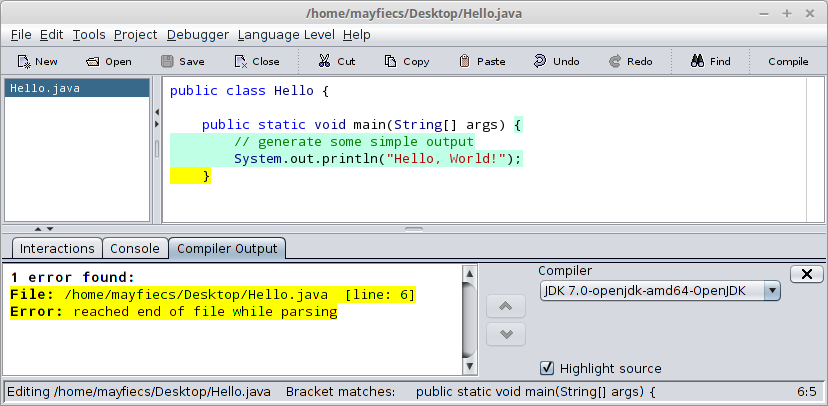
\includegraphics[width=\textwidth]{figs/syntax-error.png}
\caption{A syntax error caused by a missing brace.}
\label{fig:syntax}
\end{center}
\end{figure}

To make matters worse, the error messages you get from the compiler are often not very helpful.
As shown in Figure~\ref{fig:syntax}, removing the closing brace on line 8 of the hello world program results in ``Error: reached end of file while parsing.''
The compiler also reports that the problem was found on line 6, which in this case is not at fault.
Since line 8 was deleted, the compiler simply reported the last line of the file.

During the first few weeks of your programming career, you will probably spend a lot of time tracking down syntax errors.
But as you gain experience, you will make fewer mistakes and find them more quickly.

\subsection{Runtime errors}

\index{runtime error}
\index{error!runtime}
%\index{type-safe}
%\index{language!type-safe}

The second type of error is a {\bf runtime error}, so called because it does not appear until after the program has started running.
In Java, these errors occur when the interpreter is executing the byte code and something goes wrong.
%Java is designed to be a {\bf type-safe} language, which means that the compiler can detect many potential errors cased by common programming mistakes.
Runtime errors are rare in the simple programs you will see in the first few chapters, so it might be a while before you encounter one.

\index{exception}

These errors are also called {\em exceptions} because they usually indicate that something exceptional (and bad) has happened.
In most environments they appear as windows or dialog boxes that contain information about what happened and what the program was doing when it happened.
For example, if you accidentally divide by zero you will get an \java{ArithmeticException}:

\begin{small}
\begin{stdout}
Exception in thread "main" java.lang.ArithmeticException: / by zero
    at Hello.main(Hello.java:5)
\end{stdout}
\end{small}

This information is useful for debugging.
The first line gives a brief description of the error (/ by zero).
The subsequent lines report the class and method names (Hello.main), along with the file name and line number where the error occurred (Hello.java:5).
Keep in mind that the line where the program crashed may not be the line that needs to be fixed.

\subsection{Logic errors}

\index{logic error}
\index{error!logic}

The third type of error is the {\bf logic error}.
If there is an error in your program's logic, it will compile and run successfully in the sense that the computer will not generate any error messages.
But it will not do the right thing.
It will do something else.
Specifically, it will do what you told it to do.
Here is an example of a logic error in the hello world program:

\begin{code}
public class Hello {

    public static void main(String[] args) {
        System.out.println("Goodbye, world.");
    }

}
\end{code}

This program compiles and runs just fine.
The problem is that the main method is not the program we intended.
The meaning of the program is wrong, because it says goodbye instead of hello.
In addition, world is not capitalized, and it ends with a period instead of an exclamation point.

Identifying logic errors can be tricky because it requires you to challenge your assumptions, both about the code and the requirements.
You will need to work backwards by looking at the output of the program, try to figure out what it is doing, and make sure you understand what it should be doing.


\section{Creating variables}

\index{variable}
\index{value}

One of the most powerful features of a programming language is the ability to define and manipulate {\bf variables}.
A variable is a named location of computer memory that stores a {\bf value}.
Values may be numbers, text, images, sounds, and other types of data.
%They can be printed, and as we'll see later, operated on.
To store a value in memory, you first have to create a variable.
%Since the values we want to store are text, we declare that the new variable is a string:

\begin{code}
    String message;
\end{code}

\index{declaration}
\index{statement!declaration}
\index{type!int}
\index{type!char}
\index{type!String}

This statement is a {\bf declaration}, because it declares that the variable named \java{message} has the type \java{String}.
Each variable has a {\bf type} that determines what kind of values it can store.
For example, the \java{int} type can store integers, and the \java{char} type can store characters.

Some types begin with a capital letter and some with lower-case.
We will learn the significance of this distinction later, but for now you should take care to get it right.
There is no such type as \java{Int} or \java{string}, and the compiler will complain if you make one up.

To declare an integer variable, the syntax is:

\begin{code}
    int x;
\end{code}

Note that \java{x} is an arbitrary name for the variable.
In general, you should use names that indicate what the variables mean.
For example, if you saw these variable declarations, you could probably guess what values would be stored in them:

\begin{code}
    String firstName;
    String lastName;
    int hour, minute;
\end{code}

This example also demonstrates the syntax for declaring multiple variables with the same type: \java{hour} and \java{minute} are both integers.
Note that each declaration statement ends with a semicolon.

You can use any name you want for a variable.
But there are certain words that are reserved in Java, because they are used by the compiler to parse the structure of the program.
These {\bf keywords} include \java{public}, \java{class}, \java{static}, \java{void}, \java{int}, and others (there are currently 50 in Java).
Search the Internet for ``Java keywords'' to see the complete list.

%The complete list is available at \url{https://docs.oracle.com/javase/tutorial/}.
%This site, provided by Oracle, includes Java documentation I refer to throughout the book.

Rather than memorize the keywords, you should take advantage of the syntax highlighting provided in many development environments (including DrJava).
As you type, the tokens in your program will appear in different colors.
For example, keywords might be blue, strings red, comments green, and other code black.
If you type a variable name and it turns blue, watch out!

\subsection{Assignment}

\index{assignment}
\index{statement!assignment}

Now that we have created variables, we want to store values.
We do that with an {\bf assignment} statement.

\begin{code}
    message = "Hello!";  // give message the value "Hello!"
    hour = 10;           // assign the value 10 to hour
    minute = 59;         // set minute to 59
    hour = 11;           // change the hour to 11
\end{code}

This example shows four assignments, and the comments illustrate different ways people sometimes talk about assignment statements.
The vocabulary can be confusing here, but the idea is straightforward:

\begin{itemize}
\item When you declare a variable, you create a named storage location.
\item When you make an assignment to a variable, you give it a value.
\item If you reassign the variable, its value changes.
\end{itemize}

As a general rule, a variable has to have the same type as the value you assign to it.
For example, you cannot store a \java{String} in \java{minute} or an integer in \java{message}.
We will see some examples that seem to break this rule, but we'll get to that later.

%On the other hand, that rule can be confusing.
%There are many ways that you can convert values from one type to another, and Java sometimes converts things automatically.
%For now you should remember the general rule, and we'll talk about exceptions later.

A common source of confusion is that some strings {\em look} like integers, but they are not.
For example, \java{message} can contain the string \java{"123"}, which is made up of the characters \java{'1'}, \java{'2'}, and \java{'3'}.
But that is not the same thing as the integer \java{123}.

\begin{code}
    message = "123";  // legal
    message = 123;    // not legal
\end{code}

\subsection{Memory diagrams}

\index{memory diagram}

A common way to represent variables on paper is to draw a box with the name of the variable on the outside and the value of the variable on the inside.
This diagram shows the effect of the four assignments in the previous section:

\begin{center}
\begin{tabular}{rl}
message & \framebox[2cm]{Hello!} \\
   hour & \framebox[1cm]{11} \\
 minute & \framebox[1cm]{59} \\
\end{tabular}
\end{center}

% ABD: In the hour box, consider showing 10 crossed out, followed by 11?

Each box represents the storage location that holds the variable's value.
Once declared, you cannot change the name of a variable, but you can change the value as many times as you like.
For example, \java{hour} was initially \java{10}, then reassigned to \java{11}.
The diagram shows only the final value.

%Since these locations can be anywhere in memory, we refer to them by the variable name.
%The storage location does not change; those memory cells are simply reused.


\section{Printing variables}
\label{sec:printvar}

You can display the value of a variable using \java{print} or \java{println}.
The following program declares a variable named \java{firstLine}, assigns it the value \java{"Hello, again!"}, and then prints that value.

\begin{code}
public class Hello {
    public static void main(String[] args) {
        String firstLine;
        firstLine = "Hello, again!";
        System.out.println(firstLine);
    }
}
\end{code}

When we talk about printing a variable, we generally mean printing the {\em value} of the variable.
To print the {\em name} of a variable, you have to put it in quotes.
%For example: \java{System.out.println("firstLine");}
For example, you can write:

\begin{code}
    String firstLine;
    firstLine = "Hello, again!";
    System.out.print("The value of firstLine is ");
    System.out.println(firstLine);
\end{code}

The output of this program is:

\begin{stdout}
The value of firstLine is Hello, again!
\end{stdout}

%The output does not contain quote marks around \java{Hello, again!}.
%Those quote marks were part of the source code, not the value.

The syntax for printing a variable is the same regardless of the variable's type.
For example:

\begin{code}
    int hour, minute;
    hour = 11;
    minute = 59;
    System.out.print("The current time is ");
    System.out.print(hour);
    System.out.print(":");
    System.out.print(minute);
    System.out.println(".");
\end{code}

The output of this program is:

\begin{stdout}
The current time is 11:59.
\end{stdout}

To output multiple values on the same line, it's common to use several \java{print} statements followed by a \java{println} at the end.
{\bf Don't forget the \java{println}!}
On many operating systems, the output from \java{print} is stored without being displayed until \java{println} is invoked, at which point the entire line is displayed at once.
If you omit the \java{println}, the program may display the stored output at unexpected times or even terminate without displaying anything.


\section{Arithmetic operators}

%Recall that Java programs are organized into {\em classes}, each of which has one or more {\em methods}, each of which has one or more {\em statements}.
%Most statements consist of one or more {\bf expressions}.

\index{operator}

{\bf Operators} are symbols that represent computations like addition and multiplication.
%Most operators in Java do what you expect them to do, since they are common mathematical symbols.
For example, the operator for addition is {\tt +}, subtraction is {\tt -}, multiplication is {\tt *}, and division is {\tt /}.
%Variables are replaced with their values before the computation is performed.

The following program converts the time of day to minutes:

\begin{code}
    int hour, minute;
    hour = 11;
    minute = 59;
    System.out.print("Number of minutes since midnight: ");
    System.out.println(hour * 60 + minute);
\end{code}

\index{expression}

In this program, \java{hour * 60 + minute} is an {\bf expression}, which represents a single value to be computed.
When the program runs, each variable is replaced by its current value, and then the operators are applied.
The result is:

\begin{stdout}
Number of minutes since midnight: 719
\end{stdout}

Expressions are generally a combination of numbers, variables, and operators.
When complied and executed, they become a single value:

\begin{code}
    1 + 1     hour - 1     hour * 60 + minute     minute / 60
    2         11 - 1       11 * 60 + 59           59 / 60
              10           660 + 59               0
                           719
\end{code}

Addition, subtraction, and multiplication all do what you expect, but you might be surprised by division.
For example, the following lines try to compute the fraction of an hour that has elapsed:

\begin{code}
    System.out.print("Fraction of the hour that has passed: ");
    System.out.println(minute / 60);
\end{code}

But the program outputs:

\begin{stdout}
Fraction of the hour that has passed: 0
\end{stdout}

\index{division!integer}
\index{integer division}

This result often confuses people.
After all, the value of \java{minute} is 59, and 59 divided by 60 should be 0.98333, not 0.
The problem here is that Java performs {\em integer division}.
When the values being divided are integers, the result is also an integer.
Computer hardware is designed so that integer division always {\em rounds down}, even in cases like this one where the next integer is close.

One solution is to calculate a percentage rather than a fraction:

\begin{code}
    System.out.print("Percent of the hour that has passed: ");
    System.out.println(minute * 100 / 60);
\end{code}

The new output is:

\begin{stdout}
Percent of the hour that has passed: 98
\end{stdout}

Again the result is rounded down, but at least now it's approximately correct.
%To get a more precise answer, we can use a different type of variable that can store fractional values.


\section{Floating-point numbers}

\index{floating-point}
\index{double (floating-point)}
\index{type!double}

A more general solution is to use {\bf floating-point} numbers, which can represent fractions as well as integers.
%As the name implies, the decimal point floats around (i.e., you can have as many decimal places as you want).

In Java, the default floating-point type is called \java{double}, which is short for double-precision.
You can create \java{double} variables and assign values to them using the same syntax we used for the other types:

\begin{code}
    double pi;
    pi = 3.14159;
\end{code}

Although floating-point numbers are useful, they can be a source of confusion.
For example, Java distinguishes the integer value \java{1} from the floating-point value \java{1.0}, even though they seem to be the same number.
They belong to different data types, and strictly speaking, you are not allowed to make assignments between types.

The following is illegal because the variable on the left is an \java{int} and the value on the right is a \java{double}.

\begin{code}
    int x;
    x = 1.1;  // syntax error
\end{code}

But it is easy to forget this rule because in many cases Java {\em automatically} converts from one type to another:

\begin{code}
    double y;
    y = 1;  // bad style
\end{code}

The above example should be illegal, but Java allows it by converting the \java{int} value \java{1} to the \java{double} value \java{1.0} automatically.
This leniency is convenient, but it often causes problems for beginners. For example:

\begin{code}
    double y;
    y = 1 / 3;  // logic error
\end{code}

\index{division!integer}
\index{integer division}

You might expect the variable \java{y} to get the value \java{0.333333}, which is a legal floating-point value.
But instead it gets the value \java{0.0}.
The reason is that the expression on the right divides two integers.
So Java does {\em integer division}, which yields the \java{int} value \java{0}.
Converted to \java{double}, the final result is \java{0.0}.

One way to solve this problem (after you finally discover that bug) is to make the right-hand side a floating-point expression.
The following initializes \java{y} to \java{0.333333}, as expected:

\begin{code}
    double y;
    y = 1.0 / 3.0;  // correct
\end{code}

As a matter of style, you should always assign floating-point values to floating-point variables.
The compiler won't make you do it, but you never know when a bug like this one will come back and haunt you.


\section{Operators for strings}

\index{string operator}
\index{operator!string}

In general, you cannot perform mathematical operations on strings, even if the strings look like numbers.
The following expressions are illegal:

\begin{code}
    "Hello" - 1     "World" / 123     "Hello" * "World"
\end{code}

%Note that it's unclear looking at these expressions whether \java{message} is an integer or a string.
%The only way to tell the type of a variable is to look at the place where it is declared.

\index{concatenate}

The {\tt +} operator does work with strings, but it might not do what you expect.
For strings, the {\tt +} operator performs {\bf concatenation}, which means joining each part end-to-end.
So \java{"Hello, " + "world!"} yields the string \java{"Hello, world!"}.
Likewise, the expression \java{"Hello, " + name} adds the value of \java{name} to the hello string, which is handy for creating a personalized greeting.

%When you append two strings, make sure one of them contains a space character.
%Otherwise you will end up with something like \java{"Hello,world!"}.

%\subsection{Adding Strings and numbers}

%If you add an \java{int} and a \java{double}, Java automatically converts the \java{int} into a \java{double} before performing the addition:

%\begin{code}
%    System.out.println(1 + 2.0);
%    // prints 3.0
%\end{code}

Since addition is defined for both numbers and strings, Java performs automatic conversions you may not expect:

% TODO: use DrJava interactive format for these examples?

\begin{code}
    System.out.println(1 + 2 + "Hello");
    // the output is 3Hello

    System.out.println("Hello" + 1 + 2);
    // the output is Hello12
\end{code}

Java executes these operations from left to right.
In the first line, \java{1 + 2} is the value \java{3}, and \java{3 + "Hello"} is the value \java{"3Hello"}.
But in the second line, \java{"Hello" + 1} is \java{"Hello1"}, and \java{"Hello1" + 2} is \java{"Hello12"}.
The difference is when the conversion from integer to string actually takes place.

%Fortunately, this situation only happens when using the plus operator.
%You cannot, for example, store an integer directly in a string variable.
%
%\begin{code}
%     String number = 5;  // syntax error
%\end{code}

%In general, it's better not to compose multiple additions of varying data types.
%Instead you can break those statements into multiple lines, or use another method like \java{printf} to achieve the same results.


% TODO: add the following subsection before/after this section?
%\section{Type conversion}
%\index{type!conversion}
%\index{typecasting}

%You might wonder how you can get away with an expression like \java{
%"The log of x is " + result}, since one of the operands is a \java{String}
%and the other is a \java{double}.  In this case Java is being
%smart on our behalf, automatically converting the \java{double} to a
%\java{String} before it does the string concatenation.

%This kind of feature is an example of a common problem in designing a
%programming language, which is that there is a conflict between {\em
%formalism}, which is the requirement that formal languages should have
%simple rules with few exceptions, and {\em convenience}, which is the
%requirement that programming languages be easy to use in practice.

%More often than not, convenience wins, which is usually good for
%expert programmers (who are spared from rigorous but unwieldy
%formalism), but bad for beginning programmers, who are often baffled
%by the complexity of the rules and the number of exceptions.  In this
%book I have tried to simplify things by emphasizing the rules and
%omitting many of the exceptions.

%Whenever you try to ``add'' two
%expressions, if one of them is a \java{String}, Java converts the
%other to a \java{String} and then perform string concatenation.
%What do you think happens if you perform an operation between
%an integer and a floating-point value?


\section{Order of operations}

\index{order of operations}
\index{precedence}

When more than one operator appears in an expression, the order of evaluation depends on the rules of {\bf precedence}.
Generally speaking, Java executes individual operations from left to right (as was the case in the previous section).
But for numeric operators, Java follows mathematical conventions:

\begin{itemize}

\item Multiplication and division happen before addition and subtraction.
So \java{2 * 3 - 1} yields 5, not 4, and \java{2 / 3 - 1} yields -1, not 1.
Remember that because of integer division, \java{2 / 3} is 0.

\item If the operators have the same precedence, they are evaluated from left to right.
So in the expression \java{minute * 100 / 60}, the multiplication happens first, yielding \java{5900 / 60}, which in turn yields \java{98}.
If these same operations had gone from right to left, the result would have been \java{59 * 1}, which is incorrect.

\item Any time you want to override the rules of precedence (or you are not sure what they are) you can use parentheses.
Expressions in parentheses are evaluated first, so \java{2 * (3 - 1)} is 4.
You can also use parentheses to make an expression easier to read, as in \java{(minute * 100) / 60}, even though it doesn't change the actual result.

\end{itemize}

Don't work too hard to remember all the rules of precedence, especially for other operators.
If it's not obvious by looking at the expression, use parentheses to make it more clear.


\section{Composition}

\index{composition}

So far we have looked at the elements of a programming language---variables, expressions, and statements---in isolation, without talking about how to put them all together.

One of the most useful features of programming languages is their ability to take small building blocks and {\bf compose} them.
For example, we know how to multiply numbers and we know how to print.
It turns out we can combine these operations into a single statement:

\begin{code}
    System.out.println(17 * 3);
\end{code}

Any expression involving numbers, strings, and variables can be used inside a print statement.
We've already seen one example:

\begin{code}
    System.out.println(hour * 60 + minute);
\end{code}

You can also put arbitrary expressions on the right side of an assignment:

\begin{code}
    int percentage;
    percentage = (minute * 100) / 60;
\end{code}

The left side of an assignment must be a {\em variable name}, not an expression.
That's because the left side indicates where the result will be stored,
and expressions do not represent storage locations.

\begin{code}
    hour = minute + 1;  // correct
    minute + 1 = hour;  // syntax error
\end{code}

\index{readability}

The ability to compose operations may not seem that impressive now, but we will see examples later on that allow us to write complex computations neatly and concisely.

Before you get too carried away with composition, keep in mind that other people will be reading your source code.
In practice, software developers spend the vast majority of their time {\em understanding} and {\em modifying} existing code.
Thus it's far more important to write code that is readable than to write code that is (or appears to be) optimal.
%There is much beauty in simplicity.
In general, each line of code should be a single step of the algorithm.


\section{Formatting and style}

\index{whitespace}

Recall from Section~\ref{sec:formatting} that the compiler generally ignores {\bf whitespace}, i.e., newlines, tab characters, and other spaces.
Programmers have a lot of freedom in how they {\em format} their code in terms of indenting, blank lines, spaces around operators, etc.
However with that freedom comes responsibility, both to yourself (when you look at the code in the future) and to others who will be reading, understanding, and modifying your code.

\index{Google style}

Virtually every organization that does a lot of software development has strict guidelines on how to format source code.
For example, Google published its Java coding standards for use in open-source projects:
\url{http://google.github.io/styleguide/javaguide.html}
It is easier to understand a large codebase when all the source code is formatted consistently.
%Plus following style guidelines helps you to avoid common programming mistakes that are difficult to debug.

\index{Checkstyle}

Style rules can be difficult to learn, especially for beginners who haven't yet seen many of the language features discussed in them.
Fortunately there are many tools that help programmers find and correct formatting errors.
One prominent example is Checkstyle, which has the built-in ability to enforce most of Google's coding standards:
\url{http://checkstyle.sourceforge.net/}

Checkstyle is primarily a command-line tool.
Instructions for downloading and running Checkstyle are available on our website: \url{http://thinkjava.org/}

% TODO: When we have the website up, let's update this with a more specific URL

There are limits to what automatic style checkers can do.
In particular, they can't evaluate the {\em quality} of your comments, the {\em meaning} of your variable names, or the {\em structure} of your algorithms.
Good comments make it easier for experienced developers to identify errors in your code.
Good variable names communicate the intent of your program and how the data is organized.
And good programs are designed to be efficient and demonstrably correct.


\section{Vocabulary}

\begin{description}

\term{syntax error}
An error in a program that makes it impossible to parse (and therefore impossible to compile).

%\term{type-safe}
%A property of Java that makes it possible to catch some errors at compile time.

\term{runtime error}
An error in a program that makes it impossible to execute completely.
In Java, they are ``exceptions'' that terminate the program.

\term{logic error}
An error in a program that makes it do something other than what the programmer intended.

\term{variable}
A named storage location for values.
All variables have a type, which is declared when the variable is created.

\term{value}
A number or string that can be stored in a variable.
Every value belongs to a type (for example, \java{int} or \java{String}).

\term{declaration}
A statement that creates a new variable and specifies its type.

\term{type}
Mathematically speaking, a set of values.
The type of a variable determines which values it can have.

\term{keyword}
A reserved word used by the compiler to parse programs.
You cannot use keywords (like \java{public}, \java{class}, and \java{void}) as variable names.

\term{assignment}
A statement that stores a value in a memory location.

\term{operator}
A symbol that represents a computation like addition, multiplication, or string concatenation.

%\term{operand}
%One of the values on which an operator operates.

\term{expression}
A combination of variables, operators, and values that represents a single value.
Expressions also have types, as determined by their operators and operands.

\term{floating-point}
A data type that represents decimal numbers (numbers that have an integer part and a fractional part).
In Java, the default floating-point type is \java{double}.

\term{concatenate}
To join two values end-to-end.
For string values, concatenation means to append.

\term{precedence}
The order in which operations are evaluated.

\term{composition}
The ability to combine simple expressions and statements into compound expressions and statements, making it possible to represent complex computations in a concise manner.

\term{whitespace}
Newlines, tab characters, and other spaces in a source program.
Its purpose in the Java language is to separate tokens.

%\term{wildcard}
%A command-line feature that allows you to specify a pattern of file names.

\end{description}


\section{Exercises}

\begin{exercise}

If you are using this book in a class, you might enjoy this exercise.
Find a partner and play {\it Stump the Chump}:

Start with a program that compiles and runs correctly.
One player turns away while the other player adds an error to the program.
Then the first player tries to find and fix the error.
You get two points if you find the error without compiling the program, one point if you find it using the compiler, and your opponent gets a point if you don't find it.

\end{exercise}

\begin{exercise}
\label{ex:date}

The point of this exercise is (1) to use string concatenation to display values with different types (\java{int} and \java{String}), and (2) to practice developing programs gradually by adding a few statements at a time.

\begin{enumerate}

\item Create a new program named {\tt Date.java}.
Copy or type in something like the ``Hello, World!'' program and make sure you can compile and run it.

\item Following the example in Section~\ref{sec:printvar}, write a program that creates variables named \java{day}, \java{date}, \java{month}, and \java{year}.
\java{day} will contain the day of the week and \java{date} will contain the day of the month.
What type is each variable?
Assign values to those variables that represent today's date.

\item Print the value of each variable on a line by itself.
This is an intermediate step that is useful for checking that everything is working so far.

\item Modify the program so that it prints the date in standard American format, for example: {\tt Thursday, July 16, 2015}.

\item Modify the program again so that the total output is:

\begin{stdout}
American format:
Thursday, July 16, 2015
European format:
Thursday 16 July, 2015
\end{stdout}

\end{enumerate}

HINT: You should be able to copy, paste, and modify the code from Step 4 when completing Step 5.

\end{exercise}

\begin{exercise}

The point of this exercise is (1) to use some of the arithmetic operators, and (2) to start thinking about compound entities (like time of day) that that are represented with multiple values.

\begin{enumerate}

\item Create a new program called {\tt Time.java}.
From now on, we won't remind you to start with a small, working program, but you should.

\item Following the example program in Section~\ref{sec:printvar}, create variables named \java{hour}, \java{minute}, and \java{second}.
Assign values that are roughly the current time.
Use a 24-hour clock, i.e., so that at 2pm the value of \java{hour} is 14.

\item Make the program calculate and print the number of seconds since the most recent midnight.

\item Make the program calculate and print the number of seconds remaining in the day.

\item Make the program calculate and print the percentage of the day that has passed.
You might run into problems when computing percentages with integers, so consider using floating-point.

\item Change the values of \java{hour}, \java{minute}, and \java{second} to reflect the current time.
Check that the program works correctly each time you run it.

\end{enumerate}

HINT: You may want to use additional variables to hold values during the computation.
Variables that are used in a computation but never printed are sometimes called intermediate or temporary variables.

\end{exercise}


\chapter{Input and output}

%A number of years ago, Jeannette Wing published a terrific editorial with the title {\it Computational Thinking}, or in her own words, ``Ways to Think Like a Computer Scientist'' (see Communications of the ACM, March 2006).
%This 3-page article summarizes many of the problem-solving techniques you will discover while learning to program.
%Everyone interested in learning computer science beyond programming should read it.
%She defines the field this way:

%\index{computer science}

%\begin{quote}
%{\bf ``Computer science is the study of computation---what can be computed and how to compute it.''}
%\end{quote}

The programs we've looked at so far just display messages, which doesn't involve a lot of real computation.
This chapter will show you how to read input from the keyboard, use that input to calculate a result, and then format that result for output.
%We will also look at some technical details about how operating systems work.


\section{The System class}
\label{sec:system}

\index{System class}
\index{class!System}

\java{System.out.println} can display the value of any type of variable.
You can even use \java{println} to print the value of \java{System.out}:

\begin{code}
    System.out.println(System.out);
\end{code}

The result is:

\begin{stdout}
java.io.PrintStream@685d72cd
\end{stdout}

\index{package}

From this output we can see that \java{System.out} is a \java{PrintStream}, which is defined in a package called \java{java.io}.
A {\bf package} is a collection of related classes; \java{java.io} contains classes for ``I/O'' which stands for input and output.

\index{address}

After the {\tt @} sign is the location of the object in memory, which is called its {\bf address}.
In this example the address is \java{685d72cd}, but if you run the same code you will likely get something different.
%You can think of the address as a unique identifier for the object.

\index{object}

\java{System.out} is an {\bf object}, which means that it is a special value that provides methods.
Specifically, \java{System.out} provides methods for displaying output, including \java{print} and \java{println}.
Numbers with type \java{int} and \java{double} are not objects because they provide no methods.
Strings are objects; we will see some of their methods soon.

\index{library}

The \java{System} class is defined in a file called {\tt System.java}, and {\tt PrintStream} is defined in {\tt PrintStream.java}.
These files are part of the Java {\bf library}, which is an extensive collection of classes you can use in your programs.

\begin{figure}[!h]
\begin{center}
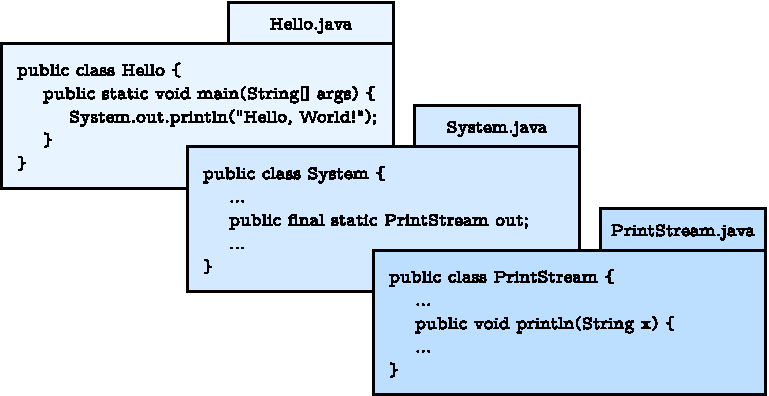
\includegraphics{figs/system.pdf}
\caption{\java{System.out.println} refers to the \java{out} variable of the \java{System} class, which is a \java{PrintStream} that provides a method called \java{println}.}
\end{center}
\end{figure}

%Both \java{System} and \java{PrintStream} are written in Java, and later in the book we'll examine their source code.
%For now, you should understand that \java{System.out} is a \java{PrintStream} object.
%Because Java is an {\em object-oriented} language, much of the library is organized around objects that perform specific actions.

% ABD: there is so much new vocab in these sections, I want to reduce the number of new ideas

%\index{operating system}

%As with most software, Java programs run on top of an {\bf operating system} that manages the keyboard, the display, main memory, disk drives, printers, the network, and other hardware resources.
%Common examples of operating systems include Android, iOS, Linux, Mac OS~X, and Windows.
%When starting Java programs, the operating system directs \java{System.out} to the screen.

%\index{abstraction}

%Note the exact type of display doesn't matter, whether it's a 5-inch touch screen or 30-inch monitor.
%From the programmer's point of view, \java{System.out} simply provides the means for printing messages.
%Computer scientists often use {\bf abstraction} to deal with the complexity of software.
%The \java{System} class is a platform-independent abstraction of the operating system.
%The operating system itself is a layer of abstraction on top of computer hardware.


\section{The Scanner class}

\index{Scanner class}
\index{class!Scanner}

%\index{byte}
%
%From the operating system's point of view, data from the keyboard arrives in a series of hardware control signals.
%The operating system translates these signals into a stream of {\bf bytes} (small integers), which in turn need to be translated into characters.
%\java{System.in} provides the means for reading one byte of input at a time, which is hardly useful for programs that would rather read in an entire word or line of input.

The \java{System} class also provides an object named \java{in}, which is an \java{InputStream} that provides methods for reading input from the keyboard.
%As with \java{System.out}, the exact type of keyboard (or even touch screen) does not matter to the programmer.
These methods perform simple operations, but they are not easy to use.
Fortunately, Java provides other classes that make it easier to handle common input tasks.

\index{class!utility}
\index{utility class}

For example, \java{Scanner} is a class that provides methods for inputting words, numbers, and other data.
\java{Scanner} is provided by \java{java.util}, which is a package that contains classes so useful they are called {\bf utility classes}.
Before you can use \java{Scanner}, you have to import it at the top of your source file:

\begin{code}
import java.util.Scanner;
\end{code}

\index{import}
\index{statement!import}

This {\bf import statement} tells the compiler that when you say \java{Scanner}, you mean the one defined in \java{java.util}.
It's necessary because there might be another class named \java{Scanner} in another package.
Using an import statement makes your code unambiguous.

Next you have to create a \java{Scanner} object using the keyword \java{new}.
%In most programs, you will need only one \java{Scanner}, since there is only one source of input.
The following code declares a \java{Scanner} variable and then creates a \java{Scanner} object:

\begin{code}
    Scanner in;
    in = new Scanner(System.in);
\end{code}

Although \java{Scanner} is not a method, the syntax is the same as a method call.
We pass \java{System.in} as an argument, which specifies that we are planning to input values from the keyboard.
Alternatively, you can declare the variable and assign it using one line of code.
%This latter syntax is more convenient, since it's a one-time setup for many programs.
%Just make sure you understand that it's two statements in one.

\begin{code}
    Scanner in = new Scanner(System.in);
\end{code}

The new \java{Scanner} object (stored in the variable \java{in}) provides a method called \java{nextLine} that reads a line of input from the keyboard and returns a String.
The following example reads two lines and repeats them back to the user.

\begin{code}
import java.util.Scanner;

public class Echo {
    public static void main(String[] args) {
        String line;
        Scanner in = new Scanner(System.in);

        System.out.print("Type something:");
        line = in.nextLine();
        System.out.println("You said: " + line);

        System.out.print("Type something else:");
        line = in.nextLine();
        System.out.println("You also said: " + line);
    }
}
\end{code}

If you omit the import statement and later refer to \java{Scanner}, you will get a compiler error like ``cannot find symbol.''
That means the compiler doesn't know what you mean by \java{Scanner}.

You might wonder why we can use the \java{System} class without importing it.
\java{System} belongs to the \java{java.lang} package, which is imported automatically.
According to the documentation, \java{java.lang} ``provides classes that are fundamental to the design of the Java programming language.''
The \java{String} class is also part of the \java{java.lang} package.

\subsection{Structure of Java programs}
\label{sec:library}

At this point, we have seen all of the elements that make up Java programs.
The following figure shows these organizational units.

\begin{figure}[!h]
\begin{center}
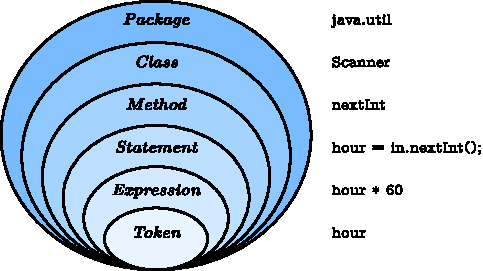
\includegraphics[width=4in]{figs/package.pdf}
\caption{Elements of the Java language, from largest to smallest.}
\end{center}
\end{figure}

To review, a package is a collection of classes, which define methods.
Methods contain statements, some of which contain expressions.
Expressions are made up of tokens, which include variable names, numbers, operators, keywords, and punctuation like braces and semicolons.

The standard edition of Java comes with {\em several thousand} classes you can \java{import}, which can be both exciting and intimidating.
You can browse this library on Oracle's website: \url{http://docs.oracle.com/javase/7/docs/api/}
Note there is a major difference between the Java {\em language}, which deals with syntax and grammar, and the Java {\em library}, which provides the built-in classes.
In fact, most of the Java library itself is written in Java.

%To help keep things organized, classes are grouped into {\bf packages}.
%Just as each \java{class} is a separate file, each \java{package} is a separate folder.

%In order to use a class defined in another package (and in another folder), you have to {\bf import} it first.

%\begin{code}
%import java.io.File;
%import java.io.PrintStream;
%import java.util.Date;
%import java.util.Scanner;
%\end{code}

%All \java{import} statements appear at the top of the source file, above the class definition.
%It's not uncommon for Java programs to have many import statements.


\section{Inches to centimeters}

Now let's see an example that's a little more useful.
Although most of the world has adopted the metric system for weights and measures, some countries are stuck with English units.
For example, when talking with friends in Europe about the weather, people in the United States may have to convert from Celsius to Fahrenheit and back.
%And when making an international purchase online, you may have to convert your nation's currency into another based on the exchange rate.
Or you might want to convert your height in inches to centimeters.

%An everyday problem that computers are great at solving is converting numbers from one unit into another.
%For the rest of the chapter, we will look at how to write programs that solve these types of problems.
%Specifically, each program will 1) prompt the user for input, 2) read input from the keyboard, 3) calculate a result, and 4) format the result for output.
%The focus will not only be on Java syntax and language features, but also on the {\em process} of solving the problem, documenting the code, and testing the solution.

We can write a program to help.
We can use a \java{Scanner} to input a measurement in inches, convert to centimeters, and then print the results.
These lines declare the variables and create the \java{Scanner}:

% ABD: I am inclined not to include comments in most of the code
% examples because (1) I think it makes the code less cluttered and
% easier to read, and (2) they are often redundant with the text.

% I understand that it would be good to demonstrate good commenting
% style.  Despite this benefit, I think it's better to leave
% them out.  But I don't feel strongly about it.

\begin{code}
    int inch;  // the input
    double cm;  // the output
    Scanner in = new Scanner(System.in);
\end{code}

The first step is to prompt the user for the input.
We'll use \java{print} instead of \java{println} so they can enter the input on the same line.

\begin{code}
    System.out.print("How many inches? ");
    inch = in.nextInt();
\end{code}

Next we multiply the number of inches by 2.54, since that's how many centimeters there are per inch.
Finally we display the results on one line, but use two print statements since it's easier to read.

\begin{code}
    cm = inch * 2.54;
    System.out.print(inch + " in = ");
    System.out.println(cm + " cm");
\end{code}

\index{magic number}

This code works, but it has a problem.
If another programmer reads this code, they might wonder where 2.54 comes from.
Numbers that appear in an expression with no explanation are called {\bf magic numbers}.
For the benefit of other programmers (and yourself in the future), it is helpful to assign magic numbers to variables with informative names:

\begin{code}
    final double cmPerInch = 2.54;
    cm = inch * cmPerInch;
    System.out.print(inch + " in = ");
    System.out.println(cm + " cm");
\end{code}

\subsection{Literals and constants}

\index{literal}

Parts of the output we have been printing (\java{" in = "}, \java{" cm"}, etc.) are {\em literal} string values.
{\bf Literals} are data embedded directly into programs.
In contrast, variables (\java{inch}, \java{cm}, etc.) are the names of values stored in memory.
The English word {\em variable} implies that this data is subject to change.

As we saw with \java{cmPerInch}, it's often useful to give names to literals that will be used throughout the program.
But when doing so, we don't want those variables to be changed accidentally because of an unexpected bug in the code.
As another example, consider the famous card game that comes with most versions of Microsoft Windows.

\begin{code}
    final String title = "Solitaire";
    final int deckSize = 52;
\end{code}

\index{final}
\index{constant}
\index{initialize}

The keyword \java{final} indicates these variables are {\bf constants} and therefore may be assigned only one time.
Constants are generally declared and {\bf initialized} on the same line of code.
%The term initialize means to assign for the first time.
If you attempt to assign \java{title} or \java{deckSize} later in the program, the compiler will report an error.
This feature helps prevent you from making mistakes.

It's good practice to create final variables for constant values, rather than repeat literal values again and again.
For one, it makes the program easier to understand.
When looking at the code, it may not be obvious what the number \java{52} means.
The name \java{deckSize} explains the programmer's intent.
Second, named constants make the program easier to maintain.
If we want to change the title from \java{"Solitaire"} to \java{"Klondike"}, we would only need to change one line of code (as opposed to every line where that title is used).


\section{Formatting output}

When printing floating-point numbers, Java automatically decides how many decimal places to display.

% ABD: What do you think of using the DrJava interpreter format to show the result of simple examples, as in the following?

\begin{code}
    System.out.print(7.0 / 3.0);
    // prints 2.3333333333333335   note: 5 is a rounding error
\end{code}

\index{printf}

\java{System.out} provides another method called \java{printf}, where the ``f'' stands for ``formatted''.
The first argument of \java{printf} is a {\em format string} that specifies how values should be displayed.
%It contains a template for the text you want to output, as well as positions where it will substitute other values.
The other arguments are the values themselves.

\begin{code}
    System.out.printf("Seven thirds = %.3f", 7.0 / 3.0);
    // prints Seven thirds = 2.333
\end{code}

\index{format specifier}

This format string contains ordinary text followed by a {\bf format specifier}, which is a special sequence that starts with a percent sign.
The format specifier \verb"%.3f" indicates that the value should be displayed as floating-point with three decimal places.
Here's an example that contains two format specifiers:

\begin{code}
   inch = 100;
   cm = inch * cmPerInch;
   System.out.printf("%d in = %f cm\n", inch, cm);
   // prints 100 in = 254.000000 cm
\end{code}

The values are matched up with the format specifiers in order, so \java{inch} is displayed as an integer (``d'' stands for ``decimal'') and \java{cm} is displayed as a floating-point number.
Format strings often end with a newline character (\verb"\n"), since \java{printf} does not append a newline like \java{println} does.

Learning \java{printf} is like learning a sub-language within Java.
There are many options, and the details can be overwhelming.
But here are some common uses, to give you an idea of how it works:

\begin{table}[!h]
\begin{center}
\begin{tabular}{|l|l|l|}
\hline
\verb"%d" & decimal integer & 12345 \\
\hline
\verb"%,d" & decimal integer with comma separators & 12,345 \\
\hline
\verb"%08d" & padded with zeros, at least 8 digits wide & 00012345 \\
\hline
\verb"%f" & floating-point & 6.789000 \\
\hline
\verb"%.2f" & floating-point {\em rounded} to 2 decimal places & 6.79 \\
\hline
\end{tabular}
\caption{Example format specifiers}
\end{center}
\end{table}

For more details, refer to the documentation of \java{java.util.Formatter}
or search the web for ``java formatting.''


\section{Centimeters to inches}
\label{sec:rounding}

Now suppose we have a measurement in centimeters and we want to round it off to the nearest inch.
It is tempting to write:

\begin{code}
    inch = cm / centPerInch;  // syntax error
\end{code}

But the result is an error---you get something like, ``Bad types in assignment: from double to int.''
The problem is that the value on the right is floating-point and the variable on the left is an integer.

%Java converts an \java{int} to a \java{double} automatically, since no information is lost in the process.
%On the other hand, going from \java{double} to \java{int} gets rid of the decimal places.
%Java doesn't perform this operation automatically in order to ensure that you are aware of the loss of the fractional part of the number.

\index{type cast}
\index{operator!cast}

The simplest way to convert a floating-point value to an integer is to use a {\bf type cast}, so called because it molds or ``casts'' a value from one shape to another.
The syntax for type casting is to put the name of the type in parentheses and use it as an operator.

\begin{code}
    double pi = 3.14159;
    int x = (int) pi;
\end{code}

%\index{truncate}

The \java{(int)} operator has the effect of converting what follows into an integer.
In this example, \java{x} gets the value \java{3}.
Converting to an integer always rounds {\em toward zero}, even if the fraction part is \java{0.999999} (or \java{-0.999999}).

Type casting takes precedence over arithmetic operations.
In this example, the value of \java{pi} gets converted to an integer first.
So the result is 60.0, not 62.

\begin{code}
    double pi = 3.14159;
    double x = (int) pi * 20.0;
\end{code}

%Operator precedence and integer truncation make type casting somewhat error-prone.

Keeping that in mind, here's how we can convert a measurement in centimeters to inches.

\begin{code}
    inch = (int) (cm / centPerInch);
    System.out.printf("%f cm = %d in\n", cent, inch);
\end{code}

The parentheses after the cast operator require the division to come before the type cast.
This result will be rounded toward zero, but we will learn in the next chapter how to round floating-point numbers to the closest integer.

\subsection{Modulus operator}

Let's take the example one step further: suppose you have a measurement in inches and you want to convert to feet and inches.
The goal is divide by 12 (the number of inches in a foot) and keep the remainder.

\index{modulus}
\index{operator!modulus}

We have already seen the division operator ({\tt /}), which computes the quotient of two numbers.
If the numbers are integers, it performs integer division.
Java also provides the {\bf modulus} operator ({\tt \%}), which divides two numbers and computes the remainder.

Assuming the following variables are integers, we can convert 76 inches to feet and inches like this:

\begin{code}
    quotient = 76 / 12;   // division
    remainder = 76 % 12;  // modulus
\end{code}

The first line yields 6.
The second line, which is pronounced ``76 mod 12,'' yields 4.
So 76 inches is 6 feet, 4 inches.

Although the modulus operator is a percent sign, you might find it helpful to think of it as a division sign ($\div$) rotated to the left.
Note that both {\tt /} and {\tt \%} perform {\em integer division}.
The reason why integer division ``rounds down'' is that the hardware computes the quotient and remainder separately.
%Many algorithms, including the example above, perform division and modulus together.

\index{divisible}
\index{extract digits}

Integer division turns out to be surprisingly useful.
For example, you can check whether one number is divisible by another: if \java{x \% y} is zero, then \java{x} is divisible by \java{y}.
You can also use modulus to ``extract'' digits from a number: \java{x \% 10} yields the rightmost digit of \java{x}, and \java{x \% 100} yields the last two digits.
Also, many encryption algorithms are based on modular arithmetic.


\section{Putting it all together}

%\begin{itemize}

%% Chapter 1
%\item Write a class and main
%\item Display simple output
%\item Compile and run programs
%\item Correct syntax errors

%% Chapter 2
%\item Declare/assign variables
%\item Create named constants
%\item Perform basic arithmetic
%\item Compose multiple operations

%% Chapter 3
%\item Browse the Java library
%\item Import Java library classes
%\item Initialize a Scanner object
%\item Get input from the keyboard
%\item Read/write documentation
%\item Format output with printf
%\item Divide and mod integers

%\end{itemize}

At this point you know enough Java to write useful programs that solve everyday problems.
You've seen how to 1) import Java library classes, 2) initialize a \java{Scanner} object, 3) get input from the keyboard, 4) format output with \java{printf}, and 5) divide and mod integers.
Now we can put them together in a complete program:

%Since we've looked at each of these topics in isolation, it's important to see how they fit together in a complete program.
%If you've been working through the examples on your computer as you've been reading (like we recommended in Section~\ref{sec:examples}), then good job!

\begin{code}
import java.util.Scanner;

/**
 * Converts centimeters to feet and inches.
 */
public class Convert {
    public static void main(String[] args) {
        double cm;
        int feet, inches;
        final double centPerInch = 2.54;
        Scanner in = new Scanner(System.in);

        // prompt the user and get the value
        System.out.print("Exactly how many cm? ");
        cm = in.nextDouble();

        // convert and output the result
        inches = (int) (cm / centPerInch);
        feet = inches / 12;
        inches = inches % 12;
        System.out.printf("%.2f cm = %d ft, %d in\n",
                          cm, feet, inches);
    }
}
\end{code}

\begin{itemize}

\item Although not required, all variables and constants are declared at the top of \java{main}.
This practice makes it easier to find their types later on and helps the reader know what data is involved in the algorithm.

\item For readability, each major step of the algorithm is separated by a blank line and begins with a comment.

\item Integer division and modulus often go together.
Notice how \java{inches} gets reassigned (which replaces its value) just before the \java{printf}.

\item When statements get long (generally wider than 80 characters), a common style convention is to break them across multiple lines.
The reader should never have to scroll horizontally.

\end{itemize}

%As an exercise, try running this code through Checkstyle.


\section{A few more details}

Now that you've had some experience with \java{double} and \java{Scanner}, there are a few unexpected behaviors we want to warn you about.

\subsection{Rounding errors}

%The operations we have seen so far---addition, subtraction, multiplication, and division---also work on floating-point values, although you might be interested to know that the underlying mechanism is completely different.
%In fact, most processors have special circuitry just for performing floating-point operations.

\index{rounding error}

On hardware, floating-point numbers are only approximately correct.
Some numbers, like reasonably-sized integers, can be represented exactly.
But repeating fractions, like $1/3$, and irrational numbers, like $\pi$, cannot.
To represent these numbers, computers have to round off to the nearest floating-point number.
The difference between the number we want and the floating-point number we get is called {\bf rounding error}.

%Notwithstanding, there is a fundamental flaw with floating-point arithmetic.
%In mathematics, there is an infinite number of real numbers.
%But computer processors are finite; they cannot represent {\em every} possible floating-point number.
%Even with double-precision, you will frequently run into problems.

\index{arithmetic!floating-point}

For example, the following two statements should be equivalent:

\begin{code}
    System.out.println(0.1 * 10);
    System.out.println(0.1 + 0.1 + 0.1 + 0.1 + 0.1
                     + 0.1 + 0.1 + 0.1 + 0.1 + 0.1);
\end{code}

But on many machines, the output is:

\begin{stdout}
1.0
0.9999999999999999
\end{stdout}

The problem is that \java{0.1}, which is a terminating fraction in base 10, is a repeating fraction in base 2.
So its floating-point representation is only approximate.
When we add up the approximations, the rounding errors accumulate.

For many applications, like computer graphics, encryption, statistical analysis, and multimedia rendering, floating-point arithmetic has benefits that outweigh the costs.
But if you need {\em absolute} precision, use integers instead.
For example, consider a bank account with a balance of \$123.45:

\begin{code}
    double balance = 123.45;  // potential rounding error
\end{code}

In this example, balances will become inaccurate over time as the variable is used in arithmetic operations like deposits and withdrawals.
The result would be angry customers and potential law suits.
You can avoid the problem by representing the balance as an integer:

\begin{code}
    int balance = 12345;      // total number of cents
\end{code}

\index{type!long}

This solution works as long as the number of cents doesn't exceed the largest integer, which is about 2 billion.
If necessary you can use \java{long} instead, which has a max value of $2^{63}-1$ (about 92 quadrillion dollars).
Hopefully nobody will ever need that much money!

\subsection{The Scanner bug}

Consider a simple program that asks users for their name and age.
Somewhere in the middle of the code, we have the following lines:

\begin{code}
    System.out.print("What is your name? ");
    name = in.nextLine();
    System.out.print("What is your age? ");
    age = in.nextInt();
    System.out.printf("Hello %s, age %d\n", name, age);
\end{code}

The output of the \java{printf} statement looks something like this:

\begin{stdout}
Hello Darth Vader, age 45
\end{stdout}

When you read a \java{String} followed by an \java{int}, everything works just fine.
But when you read an \java{int} followed by a \java{String}, something strange happens.

\begin{code}
    System.out.print("What is your age? ");
    age = in.nextInt();
    System.out.print("What is your name? ");
    name = in.nextLine();
    System.out.printf("Hello %s, age %d\n", name, age);
\end{code}

Try running the above example.
It doesn't let you input your name and immediately displays the output:

\begin{stdout}
What is your name? Hello , age 45
\end{stdout}

To understand what is happening, recall that computers do not {\em see} input as multiple lines like we do.
Instead, the operating system simply forwards a stream of characters to your program via \java{System.in}:

\begin{center}
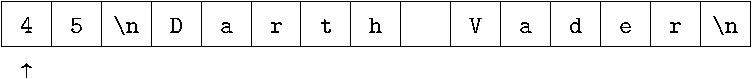
\includegraphics{figs/vader1.pdf}
\end{center}

The up-arrow represents the next character to be read by \java{Scanner}.
When you call \java{nextInt}, it will read characters until a non-digit is found.

\begin{center}
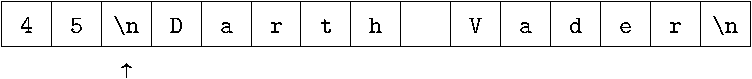
\includegraphics{figs/vader2.pdf}
\end{center}

At this point, \java{nextInt} returns the \java{int} value \java{45}.
The program then asks \java{"What is your name? "} and calls \java{nextLine}.
\java{Scanner} will read characters until a newline is found.
Since the next character to be read already is a newline, \java{nextLine} returns the empty string \java{""}.

To solve this problem, you need to add an extra call to \java{nextLine} after you call \java{nextInt}.

\begin{code}
    System.out.print("What is your age? ");
    age = in.nextInt();
    in.nextLine();  // read the newline
    System.out.print("What is your name? ");
    name = in.nextLine();
    System.out.printf("Hello %s, age %d\n", name, age);
\end{code}

This technique is common when reading \java{int} or \java{double} values that appear on their own line.
First you read the number, then you read the rest of the line (which is just a newline character).
Note that you do not have to assign the return value of \java{nextLine} to a variable in that case; you can simply ignore it.


\section{Command-line testing}

You should review the advice in Section~\ref{sec:examples}, now that you've written some more substantial programs.
Remember, it's more effective to program and debug your code little by little than to attempt writing everything at once.
And once you've completed programming an algorithm, it's important to test that it works correctly on a variety of inputs.

Throughout the book, we will illustrate techniques for testing your programs.
Most if not all testing is based on a simple idea: does the program do what we expect it to do?
For simple programs, it's not difficult to run them several times and see what happens.
But at some point, you will get tired of typing the same test cases over and over.

We can automate the process of entering input and comparing {\em expected output} with {\em actual output} using the command-line.
The basic idea is to store the test cases in plain text files and trick Java into thinking they are coming from the keyboard.
Here are step by step instructions.

\begin{enumerate}

\item Make sure you can compile and run the {\tt Convert.java} example in the previous section.
%You can also download a copy from \url{http://thinkjava.org/}.

\item In the same directory as {\tt Convert.java}, create a plain text file named {\tt test.in} (``in'' is for input).
Enter the following line and save the file.

\begin{stdout}
193.04
\end{stdout}

\item Create a second plain text file named {\tt test.exp} (``exp'' is for expected).
Enter the following line and save the file.

\begin{stdout}
193.04 cm = 6 ft, 4 in
\end{stdout}

\item Open a command-line, and change to the directory with these files.
Run the following command to test the program.

\begin{stdout}
java Convert < test.in > test.out
\end{stdout}

\end{enumerate}

\index{redirection operator}

On the command-line, {\tt <} and {\tt >} are {\bf redirection operators}.
The first one redirects the contents of {\tt test.in} to \java{System.in}, as if it were entered from the keyboard.
The second one redirects the contents of \java{System.out} to a new file {\tt test.out}, much like a screen capture.
In other words, the {\tt test.out} file contains the output of your program.

By the way, it's perfectly okay to compile your programs in DrJava (or some other environment) and run them from the command-line.
Knowing both techniques allows you to use the right tool for the job.

At this point, we just need to compare the contents {\tt test.out} with {\tt test.exp}.
If the files are the same, then the program outputted what we expected it to output.
If not, then we found a bug, and we can use the output to begin debugging our program.
Fortunately, there's a simple way to compare files on the command-line:

\begin{stdout}
diff test.exp test.out
\end{stdout}

The {\tt diff} utility summarizes the differences between two files.
If there are no differences, then it prints nothing, which in our case is what we want.
If the expected output differs from the actual output, then we need to debug our program.
Or in some cases, we need to debug our test cases.
There's always a chance we have a correct program and a typo in the expected output.

% ABD: Since I killed the previous reference to abstraction, I am inclined
% to kill this one too.  The problem in both places is that it pulls the
% focus off topic.

%Redirecting a program's input and output is an example of how computer scientists use abstraction.
%Notice that \java{System.in} is not called \java{Keyboard}, and \java{System.out} is not called \java{Display}.
%In practice, these objects could be text files, network connections, microphones and speakers, or some other byte streams.
%What's great is that doesn't change anything about how you write the code.


\section{Vocabulary}

\begin{description}

\term{package}
A group of classes that are related to each other.
Java classes are organized into packages.

\term{address}
The storage location of a variable or object in memory.
Addresses are integers encoded in hexadecimal (base 16).

\term{object}
An abstract entity that represents data and performs actions.
In Java, objects are stored in memory and referenced by variables.

\term{library}
A collection of packages and classes that are available for use in other programs.
Libraries are often distributed in {\tt .jar} (Java Archive) files.

%\term{operating system}
%Software that is always running behind the scenes on your computer.
%It controls the execution of application programs and manages hardware resources.

%\term{abstraction}
%The process of reducing information and/or detail to focus on high-level concepts.

%\term{byte}
%A single unit of data on a computer; enough to represent one character.

\term{utility class}
A class that provides commonly needed functionality.

\term{import}
A statement that allows programs to use classes defined in other packages.

\term{magic number}
A unique value with unexplained meaning or multiple occurrences.
They should generally be replaced with named constants.

\term{literal}
A constant value written directly in the source code.
For example, \java{"Hello"} is a string literal and \java{74} is an integer literal.

\term{constant}
A variable that can only be assigned one time.
Once initialized, its value cannot be changed.

\term{initialize}
To assign an initial value to a variable.

\term{format specifier}
A special code beginning with percent sign and ending with a single letter that stands for the data type.

\term{type cast}
An operation that explicitly converts one data type into another, sometimes with loss of information.
In Java it appears as a type name in parentheses, like \java{(int)}.

%\term{truncate}
%To make shorter by cutting something off.
%Casting a floating-point value to an integer simply removes the fractional part.

\term{modulus}
An operator that yields the remainder when one integer is divided by another.
In Java, it is denoted with a percent sign (e.g., \java{5 \% 2} is \java{1}).

\term{rounding error}
The small difference between a floating-point number and its actual representation on computer hardware.

\term{redirection operator}
A command-line feature that substitutes \java{System.in} and/or \java{System.out} with a plain text file.

\end{description}


\section{Exercises}

\begin{exercise}
When you use \java{printf}, the Java compiler does not check your formatting string.
See what happens if you try to display value with type \java{int} using \verb"%f".
And what happens if you display a \java{float} using \verb"%d"?
What if you use two format specifiers, but then only provide one value?
\end{exercise}


\begin{exercise}

TODO

\end{exercise}


\begin{exercise}

TODO

\end{exercise}


\chapter{Void methods}

So far we've only written short programs that have a single class with a \java{main} method.
In this chapter, we'll show you how to organize longer programs into multiple methods and classes.
%We will also take a look at separate compilation.

\index{method}

% ABD: In theory I like the idea of providing a chapter overview, but
% in practice I find them impossible to write without breaking the rules
% (like using terms before defining them, etc)

At a conceptual level, a {\bf method} represents a mathematical {\em function} or a general {\em procedure}.
Some methods perform a computation and return a result.
For example, \java{Math.sqrt(25)} returns the value \java{5.0}.
Other methods (including \java{main}) carry out a sequence of actions without returning a result.
Java uses the keyword \java{void} to declare such methods.
Regardless whether they return a value or not, methods enable you to break down a complex program into smaller blocks of code.


\section{Math methods}

\index{Math class}
\index{class!Math}
\index{expression}
\index{argument}

In mathematics, you have probably seen functions like $\sin$ and $\log$, and you have learned to evaluate expressions like $\sin(\pi/2)$ and $\log(1/x)$.
First, you evaluate the expression in parentheses, which is called the {\bf argument} of the function.
Then you can evaluate the function itself, maybe by punching it into a calculator.

This process can be applied repeatedly to evaluate more complex expressions like $\log(1/\sin(\pi/2))$.
First we evaluate the argument of the innermost function, then evaluate the function itself, and so on.

The Java library includes a \java{Math} class that provides most common mathematical operations.
%These functions are called {\bf methods}.
\java{Math} is in the \java{java.lang} package, so you don't have to import it.
You can invoke Math methods like this:

\begin{code}
    double root = Math.sqrt(17.0);
    double angle = 1.5;
    double height = Math.sin(angle);
\end{code}

The first line sets \java{root} to the square root of 17.
The third line finds the sine of the value of \java{angle}.

\index{degrees}
\index{radians}

Arguments of the trigonometric functions---\java{sin}, \java{cos}, and \java{tan}---should be in {\em radians}.
To convert from degrees to radians, you can divide by 180 and multiply by $\pi$.
Conveniently, the \java{Math} class provides a \java{final double} named \java{PI} that contains an approximation of $\pi$:

\begin{code}
    double degrees = 90;
    double angle = degrees / 180.0 * Math.PI;
\end{code}

Notice that \java{PI} is in capital letters.
Java does not recognize \java{Pi}, \java{pi}, or \java{pie}.
Also, \java{PI} is the name of a variable, not a method, so it doesn't have parentheses.
The same is true for the constant \java{Math.E}, which approximates Euler's number.

It turns out that converting to/from radians is a common operation, so the \java{Math} class provides methods for that.

\begin{code}
    double radians = Math.toRadians(180.0);
    double degrees = Math.toDegrees(Math.PI);
\end{code}

\index{type!long}

If you haven't already, take a look at the documentation for \java{Math} so you know what methods are provided.
For example, another useful method is \java{round}, which rounds a floating-point value to the nearest integer and returns a \java{long}.

\begin{code}
    long x = Math.round(Math.PI * 20.0);
\end{code}

In Java, \java{int} values are stored using 32 bits (4 bytes) of memory, whereas \java{long} values are stored in 64 bits (8 bytes).
As a result, \java{long} variables can represent much larger integers.
In the above example, the multiplication happens first, before the method is invoked.
The result is 63 (rounded up from 62.8319).

\subsection{Composition revisited}

\index{composition}
\index{expression}

Just as with mathematical functions, Java methods can be {\bf composed}.
That means you can use one expression as part of another.
For example, you can use any expression as an argument to a method:

\begin{code}
    double x = Math.cos(angle + Math.PI / 2);
\end{code}

This statement takes the value \java{Math.PI}, divides it by two, and then adds the result to the value of the variable \java{angle}.
The sum is then passed as an argument to \java{cos}.
You can also take the result of one method and pass it as an argument to another:

\begin{code}
    double x = Math.exp(Math.log(10.0));
\end{code}

In Java, the \java{log} method always uses base $e$.
So this statement finds the log base $e$ of 10, and then raises $e$ to that power.
The result gets assigned to \java{x}.
%Do you know what it is without reaching for a calculator?

When using \java{Math} methods, it is a common error to forget to specify the class name \java{Math}.
For example, \java{Math.pow} takes two arguments and raises the first argument to the power of the second.

\begin{code}
    pow(2.0, 10.0);  // syntax error
\end{code}

If you try to invoke \java{Math.pow} this way, the compiler will say it ``cannot find symbol'' (i.e., there is no method named \java{pow} in the current class).


\section{Adding new methods}
\label{adding_methods}

\index{method!definition}
\index{main}
\index{method!main}

Like the \java{Math} class, you can write your own set of methods for use in other programs.
%One of the most powerful features of a programming language is the ability to add new methods.
Let's revisit the method definition for \java{main}:

\begin{code}
    public static void main(String[] args) {
        System.out.println("Hello, World!");
    }
\end{code}

\index{public}
\index{void}
\index{type!void}

The first line contains information about the method:
\java{main} is a \java{public} method, which means it can be invoked from other classes;
it is a \java{static} method, but we're not going to explain what that means yet;
and it is a \java{void} method, which means that it doesn't yield a result (unlike the \java{Math} methods).

\index{parameter}

The statement in parentheses declares a parameter named
\java{args}.  A {\bf parameter} is a variable that stores an argument.
This parameter has type \java{String[]}, which means that whoever invokes \java{main} must provide an array of Strings (we'll get to arrays in a later chapter).

You can define other methods using syntax that is similar to \java{main}:

\begin{code}
    public static void NAME(PARAMETERS) {
        STATEMENTS
    }
\end{code}

By convention, methods start with a lower case letter and use ``camel case,'' which is a cute name for \java{jammingWordsTogetherLikeThis}.
You can use any name you want for your method, except \java{main} or any of the Java keywords.

% TODO: check where there first use of ``invoke'' was
% TODO: move the definition of ``argument'' to Ch3?

The list of parameters specifies what values, if any, you have to provide in order to invoke the new method.
The first methods we are going to write have no parameters, so the parameter list is empty.  Here's an example:

\begin{code}
    public static void newLine() {
        System.out.println();
    }
\end{code}

The name of this method is \java{newLine}.
It contains only one statement, which prints a blank line.
In \java{main}, we can invoke the new method like this:

\begin{code}
    public static void main(String[] args) {
        System.out.println("First line.");
        newLine();
        System.out.println("Second line.");
    }
\end{code}

Because \java{newLine} is in the same class as \java{main}, we don't have to specify the class name.
The output of this program is:

\begin{stdout}
First line.

Second line.
\end{stdout}

Notice the extra space between the lines.
If we wanted more space between them, we could invoke the same method repeatedly:

\begin{code}
    public static void main(String[] args) {
        System.out.println("First line.");
        newLine();
        newLine();
        newLine();
        System.out.println("Second line.");
    }
\end{code}

Or we could write a new method that prints three blank lines:

\begin{code}
    public static void threeLine() {
        newLine();
        newLine();
        newLine();
    }

    public static void main(String[] args) {
        System.out.println("First line.");
        threeLine();
        System.out.println("Second line.");
    }
\end{code}

You can invoke the same method more than once, and you can have one method invoke another.
In this example, \java{main} invokes \java{threeLine}, and \java{threeLine} invokes \java{newLine}.

%In \java{threeLine} I wrote three statements all on the same line, which is syntactically legal (remember that spaces and new lines usually don't change the meaning of a program).
%It is usually a good idea to put each statement on its own line, but I sometimes break that rule.

You might wonder why it is worth the trouble to create new methods.
There are many reasons, but this example demonstrates a few of them:

\begin{enumerate}

\item Creating a new method gives you an opportunity to give a name to a group of statements, which makes code easier to read and understand.
%Methods simplify a program by hiding complex computations behind a single statement, and by using English words in place of arcane code.
%Which is clearer, \java{newLine} or \java{System.out.println()}?

\item Introducing new methods can make a program smaller by eliminating repetitive code.
For example, to print nine consecutive new lines, you could invoke \java{threeLine} three times.

\item A common problem-solving technique is to break things down into sub-problems.
Methods allow you to focus on each sub-problem in isolation, and then compose them into a complete solution.

\end{enumerate}

%Perhaps most importantly, organizing your code into multiple methods allows you to test individual parts of your program separately.
%It's easier to get a complex program working if you know that each sub-part works correctly.

%In Section~\ref{methods} we will come back to this question and list some additional benefits of dividing programs into methods.


\section{Classes and methods}

\index{class}
\index{method}

Pulling together the code from the previous section, the complete program looks like this:

\begin{code}
public class NewLine {

    public static void newLine() {
        System.out.println();
    }

    public static void threeLine() {
        newLine();
        newLine();
        newLine();
    }

    public static void main(String[] args) {
        System.out.println("First line.");
        threeLine();
        System.out.println("Second line.");
    }
}
\end{code}

\index{case-sensitive}

The first line is the class definition.
Class names should be capitalized; this convention helps readers tell the difference between classes and methods in your source code.
The \java{NewLine} class contains three \java{void} methods: \java{newLine}, \java{threeLine}, and \java{main}.
Java is a case-sensitive language, so \java{NewLine} and \java{newLine} are considered different.

\subsection{Programs with multiple methods}

\index{order of execution}

When you look at a class definition that contains several methods, it is tempting to read it from top to bottom.
But that is likely to be confusing, because that is not the {\bf order of execution} of the program.

Execution always begins at the first statement of \java{main}, regardless of where it is in the source file.
In the previous example, we deliberately put \java{main} at the bottom of the program.
Statements are executed one at a time, in order, until you reach a method invocation.
Think of method invocations as a detour in the flow of execution.
Instead of going to the next statement, you go to the first line of the invoked method, execute the statements there, and then come back and pick up again where you left off.

That sounds simple enough, but remember that one method can invoke another one.
In the middle of \java{main}, we go off to execute the statements in \java{threeLine}.
But while we are executing \java{threeLine}, we go off to execute \java{newLine}.
Then \java{newLine} invokes \java{println}, which causes yet another detour.

Fortunately, Java is adept at keeping track of where it is.
So when \java{println} completes, it picks up where it left off in \java{newLine}, and then gets back to \java{threeLine}, and then finally gets back to \java{main} so the program can terminate.
In summary, when you read a program, don't read from top to bottom.
Instead, follow the flow of execution.

%Technically, the program does not terminate at the end of \java{main}.
%Instead, execution picks up where it left off in the program that invoked \java{main}, which is the Java interpreter.
%The interpreter takes care of things like deleting windows and general cleanup, and {\em then} the program terminates.


\section{Parameters and arguments}

\index{parameter}
\index{argument}

Some of the methods we have used require arguments, which are values that you provide when you invoke the method.
For example, to find the sine of a number, you have to provide the number.
So \java{sin} takes a \java{double} as an argument.
To print a message, you have to provide the string.
So \java{println} takes a \java{String} as an argument.
Some methods take more than one argument.
For example, \java{Math.pow} takes two \java{double}s: the base and the exponent.

When you use a method, you provide the arguments.
When you write a method, you list the parameters.
The parameter list indicates what arguments are required.
Here's a method that takes a string and prints it twice:

\begin{code}
    public static void printTwice(String s) {
        System.out.println(s);
        System.out.println(s);
    }
\end{code}

\java{printTwice} has a parameter named \java{s} with type \java{String}.
The parameter name hints that it is a \java{String}, but you could use any legal variable name.
When we invoke \java{printTwice}, we have to provide an argument with type \java{String}.
Before the method executes, the argument gets assigned to the parameter.

In this example, the argument \java{"Don't make me say this twice!"} gets assigned to the parameter \java{s}.

\begin{code}
    printTwice("Don't make me say this twice!");
\end{code}

\index{parameter passing}

This process is called {\bf parameter passing} because the value gets passed from outside the method to the inside.
An argument can be any kind of expression, so if you have a \java{String} variable, you can use it as an argument:

\begin{code}
    String argument = "Never say never.";
    printTwice(argument);
\end{code}

The value you provide as an argument must have the same type as the parameter.
For example, if you try:

\begin{code}
    printTwice(17);  // syntax error
\end{code}

You will get the compiler error ``cannot find symbol,'' which might be confusing.
Java is looking for a method named \java{printTwice} that can take an integer.
Since there isn't one in the current class, Java can't find such a ``symbol.''

There are some apparent exceptions to this rule, because sometimes Java converts from one type to another automatically.
For example, \java{Math.sqrt} requires a \java{double} value.
If you run \java{Math.sqrt(25)}, the interger value \java{25} is automatically converted to the floating-point value \java{25.0}.

\java{System.out.println} can accept any type as an argument.
But generally speaking, that is an exception; most methods are not so accommodating.

\subsection{Methods with multiple parameters}
\label{time}

\index{parameter!multiple}
\index{method!multiple parameter}
\index{class!Time}

The syntax for declaring and invoking methods with multiple parameters is a common source of confusion.
For one, you have to declare the type of every parameter separately.

\begin{code}
    public static void printTime(int hour, int minute) {
        System.out.print(hour);
        System.out.print(":");
        System.out.println(minute);
    }
\end{code}

It might be tempting to write ``\java{int hour, minute}'' but that format is only legal for variable declarations, not parameter lists.
Another common source of confusion is that you do not have to declare the types of arguments in a method call.
The following is incorrect:

\begin{code}
    int hour = 11;
    int minute = 59;
    printTime(int hour, int minute);  // syntax error
\end{code}

In this case, Java can tell the type of \java{hour} and \java{minute} by looking at their declarations.
It is unnecessary (and therefore not allowed) to include the type when you pass them as arguments.
The correct syntax is:

\begin{code}
    printTime(hour, minute);
\end{code}

When you call a method, Java {\it copies the value} of any arguments you provide into the method's parameters.
It's common for two methods (e.g., \java{main} and \java{printTime}) to have variables with the same name, to show how data passes from one method to the next.
But remember that these variables are stored in different memory locations.
Changing the value of \java{hour} or \java{minute} in \java{printTime} has no effect on the original variables in \java{main}.


\section{Reading documentation}
\label{sec:apidocs}

\index{documentation}

For a comprehensive example of what methods are like, take a look at the documentation for \java{Scanner}.
You can find it in the Java library (see the link in Section~\ref{sec:library}) or simply do a web search for ``java scanner.''
The latter technique is more useful in the long run, especially as Oracle releases new versions of Java.
Either way, you should get something like Figure~\ref{fig:javadoc}.

\begin{figure}[!h]
\begin{center}
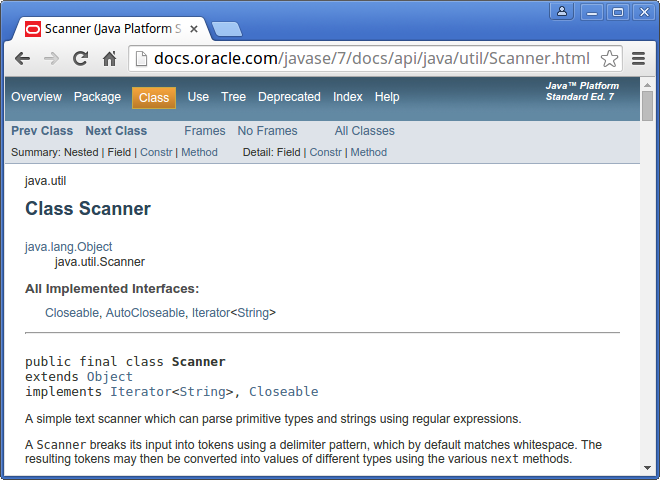
\includegraphics[width=0.9\textwidth]{figs/scanner.png}
\caption{Screenshot of the documentation for \java{Scanner} on Oracle's website.}
\label{fig:javadoc}
\end{center}
\end{figure}

Scroll down to the ``Method Summary'' section.
In the previous chapter, we introduced methods for reading the ``next'' input.
As you can see, the \java{Scanner} class provides quite a few of them.
Click on the link for \java{nextInt}, and it will scroll down to more details:

\begin{stdout}
public int nextInt()
Scans the next token of the input as an int.
\end{stdout}

\index{signature}

The first line is the method's {\bf signature}, which specifies the name of the method, its return type, and parameters.
In this example, \java{nextInt} returns an \java{int}.
The empty parentheses mean that \java{nextInt} has no parameters.
The next line explains what the method does.
The subsequent lines (not shown) describe each parameter (if any) and the return value.
Explanations are often redundant, but the documentation is supposed to fit this standard format.
%The last line describes the exceptions this method might throw.

It might take some time to get comfortable reading this kind of information, but it's well worth the effort.
Knowing what methods a class provides helps you avoid reinventing the wheel.
Whenever you learn about a new class, you should take a quick look at its documentation.
On that note, take a few minutes to review the documentation for \java{System} and \java{String}.


\section{Writing documentation}

\index{Javadoc}

A nice feature of the Java language is the ability to write documentation at the same time you are writing the source code.
That way, the documentation stays in sync with the classes and methods themselves.
In fact, the HTML pages you browsed in the previous section were automatically generated using a tool called {\bf Javadoc}.
This tool is part of the standard JDK, and you can run it directly from DrJava by pressing the {\tt Javadoc} button on the toolbar.

\index{comments!documentation}
\index{documentation comments}

Javadoc parses your source files for {\bf documentation comments} and extracts other relevant information about your class and method definitions.
Given the prevalence of this tool, people sometimes refer to documentation as ``Javadoc comments.''
In contrast to inline comments that begin with {\tt //}, documentation comments begin with {\tt /**} (two stars) and end with {\tt */} (one star).
Anything in between these two tokens becomes part of the documentation.
%As a rule of thumb, you should document every class and every method.

\begin{code}
/**
 * Example program that demonstrates print vs println.
 */
public class Goodbye {

    /**
     * Application entry point; simply prints a greeting.
     */
    public static void main(String[] args) {
        System.out.print("Goodbye, ");  // note the space
        System.out.println("cruel world");
    }

}
\end{code}

This example has perhaps too many comments, since all the program does is print a single message.
But it illustrates the differences between inline and documentation comments:

\begin{itemize}
\item Inline comments tend to be short phrases that help explain complex parts of a method.
Documentation comments are typically complete sentences that begin with a capital letter and end with a period.

\item Documentation comments often span multiple lines.
By convention, each line begins with a {\tt *} that is aligned vertically with the start and end of the comment.

\item Some development environments (e.g., Eclipse and NetBeans) automatically display documentation comments when you hover your mouse over the name of a class or method.

\end{itemize}

Writing documentation and inline comments is essential for making source code readable.
As we discussed in an earlier chapter, people spend the majority of their development time understanding and modifying existing code.
You should not only write good comments for others, but for yourself as well.
When you haven't looked at your own code for a while, it takes a long time to remember how it works (or what you were trying to do) if there's no comments.


\section{Stack diagrams and scope}
\label{stack}

\index{stack diagram}
\index{diagram!stack}

Pulling together the code examples from the previous section, here is a complete
class definition:

\begin{code}
public class PrintTwice {

    public static void printTwice(String s) {
        System.out.println(s);
        System.out.println(s);
    }

    public static void main(String[] args) {
        String argument = "Never say never.";
        printTwice(argument);
    }

}
\end{code}

Parameters and other variables only exist inside their own methods.
Within the confines of \java{main}, there is no such thing as \java{s}.
If you try to use it there, the compiler will complain.
Similarly, inside \java{printTwice} there is no such thing as \java{argument}.
That variable belongs to the \java{main} method.

One way to keep track of where each variable is defined is to draw a {\bf stack diagram}.
The stack diagram for this example looks like this:

\begin{figure}[!h]
\begin{center}
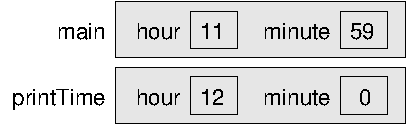
\includegraphics{figs/stack.pdf}
\caption{Stack diagram for the \java{PrintTwice} program.}
\end{center}
\end{figure}

\index{frame}

For each method there is a box called a {\bf frame} that contains the method's parameters and variables.
The name of the method appears outside the frame.
The value of each variable is drawn inside a box with the name of the variable beside it.
(Note for people who know too much: this diagram leaves out a detail we will explain later.)

Stack diagrams help you to visualize the {\bf scope} of a variable, which is the area of a program where a variable exists.
It's possible to have two variables with the same name in two different methods.
Each only exists within its own method, so they don't interfere with each other.


\section{Tracing with a debugger}

\index{debugger}

Keeping track of variables and methods on paper is a useful skill, and you should practice drawing stack diagrams.
Another way to visualize the scope of variables and the flow of execution is to use a {\bf debugger}.
The overall process is the same, regardless which development environment you use:

\index{breakpoint}

\begin{enumerate}
\item Set {\bf breakpoints} on lines where you want the program to pause.
\item Step through the code one line at a time and watch what it does.
\item Check the values of variables and see when they change.
\end{enumerate}

For example, open any program in DrJava and move the cursor to the first line of \java{main}.
Press Ctrl+B to toggle a breakpoint on the current line; it should now be highlighted in red.
Press Ctrl+Shift+D to turn on Debug Mode; a new pane should appear at the bottom of the window.
(These commands are also available from the {\em Debugger} menu, in case you forget the shortcut keys.)

\index{call stack}

When you run the program, execution pauses at the first breakpoint.
The debug pane shows the {\bf call stack}, with the current method on top of the stack.
You might be surprised to see how many methods were called before the \java{main} method!
To the right are several buttons that allow you to step through the code at your own pace.
You can also press ``Automatic Trace'' to watch DrJava run your code one line at a time.

\begin{figure}[!h]
\begin{center}
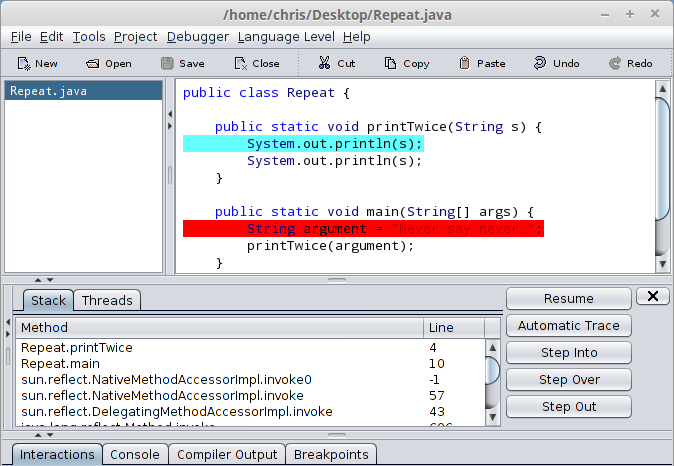
\includegraphics[width=\textwidth]{figs/debugger.png}
\caption{Screenshot of the DrJava debugger.
Execution is currently paused on the first line of \java{printTwice}.
There is a breakpoint on the first line of \java{main}.}
\end{center}
\end{figure}

When the program is paused, you can examine (or even change) the value of any variable using the Interactions Pane.
This feature allows you to verify your assumptions about how data is passed from one method to another.
You can edit your code while debugging it, but the changes won't take effect until after you compile.
The result can be confusing, so we don't recommend it.
%The debugger may get out of sync if you add or delete multiple lines of code while the program is paused.

Using a debugger is like having the computer proofread your code out loud.
You might expect the code do one thing, and then the debugger shows it doing something else.
At that moment, you gain insight about what may be wrong with the code.


\section{Vocabulary}

\begin{description}

% Note: expanded definition from Chapter 1
\term{method}
A named sequence of statements that performs a procedure or function.
Methods may or may not take parameters, and may or may not return a value.

\term{invoke}
To call a method, i.e., cause it to execute.

\term{parameter}
A piece of information a method requires before it can run.
Parameters are variables: they contain values and have types.

\term{argument}
A value that you provide when you invoke a method.
This value must have the same type as the corresponding parameter.

% Note: expanded definition from Chapter 2
\term{composition}
The ability to combine simple expressions and statements into compound expressions and statements, making it possible to use intermediate computations as arguments.

\term{order of execution}
The order in which Java executes methods and statements.
It may not necessarily be from top to bottom, left to right.

\term{parameter passing}
The process of assigning an argument value to a parameter variable.

\term{signature}
The first line of a method that defines its name, return type, and parameters.

\term{Javadoc}
A tool that reads Java source code and generates documentation in HTML format.

\term{documentation}
Comments that describe the technical operation of a class or method.

\term{stack diagram}
A memory diagram that shows which variables belong to which methods at a certain point in the program.
The methods calls are ``stacked'' from top to bottom, in the order of execution.

\term{frame}
A structure (represented by a box in stack diagrams) that contains a method's parameters and variables.

\term{scope}
The area of a program where a variable exists.

\term{debugger}
A tool that allows you to run one statement at a time and see the contents of variables.

\term{breakpoint}
A line of code where the debugger will pause a running program.

\term{call stack}
The history of method calls and where to resume execution after each method returns.

\end{description}


\section{Exercises}

\begin{exercise}

What is the difference between a variable and a method?
In terms of their syntax, how does the Java compiler tell the difference between the two?

%A variable is a {\em location of data}, whereas a method is a {\em location of code}.
%In Java, methods always have parentheses, even if they have no arguments like \java{System.out.println()}.

\begin{exercise}

Draw a stack diagram that shows the state of the program in Section~\ref{time} when \java{main} invokes \java{printTime} with the arguments \java{11} and \java{59}.

\end{exercise}

\end{exercise}

\begin{exercise}

The point of this exercise is to practice reading code and to make sure that you understand the flow of execution through a program with multiple methods.

\begin{enumerate}

\item What is the output of the following program?
Be precise about where there are spaces and where there are newlines.

HINT: Start by describing in words what \java{ping} and \java{baffle} do when they are invoked.

\item Draw a stack diagram that shows the state of the program the first time \java{ping} is invoked.

\item What happens if you add a method call to \java{baffle();} at the end of the \java{ping} method? (We will see why in the next chapter.)

\end{enumerate}

\begin{code}
    public static void zoop() {
        baffle();
        System.out.print("You wugga ");
        baffle();
    }

    public static void main(String[] args) {
        System.out.print("No, I ");
        zoop();
        System.out.print("I ");
        baffle();
    }

    public static void baffle() {
        System.out.print("wug");
        ping();
    }

    public static void ping() {
        System.out.println(".");
    }
\end{code}

\end{exercise}

\begin{exercise}

The point of this exercise is to make sure you understand how to write and invoke methods that take parameters.

\begin{enumerate}
\item Write the first line of a method named \java{zool} that takes three parameters: an \java{int} and two \java{Strings}.

\item Write a line of code that calls \java{zool}, passing as arguments the value \java{11}, the name of your first pet, and the name of the street you grew up on.
\end{enumerate}

\end{exercise}

\begin{exercise}

The purpose of this exercise is to take code from a previous exercise and encapsulate it in a method that takes parameters.
You should start with a working solution to Exercise~\ref{ex:date}.

\begin{enumerate}

\item Write a method called \java{printAmerican} that takes the day, date, month and year as parameters and that prints them in American format.

\item Test your method by invoking it from \java{main} and passing appropriate arguments.
The output should look something like this (except that the date might be different):

\begin{stdout}
Saturday, July 16, 2011
\end{stdout}

\item Once you have debugged \java{printAmerican}, write another method called \java{printEuropean} that prints the date in European format.

\end{enumerate}
\end{exercise}


%\chapter{Iteration and loops}
\label{chap06}

\section{Multiple assignment}
\index{assignment}
\index{statement!assignment}
\index{multiple assignment}

You can make more than one assignment to the same variable;
the effect is to replace the old value with the new.

\begin{code}
    int liz = 5;
    System.out.print(liz);
    liz = 7;
    System.out.println(liz);
\end{code}

The output of this program is {\tt 57}, because the first
time we print {\tt liz} her value is 5, and the second time
her value is 7.

This kind of {\bf multiple assignment} is the reason I
described variables as a {\em container} for values.  When
you assign a value to a variable, you change the contents of
the container, as shown in the figure:


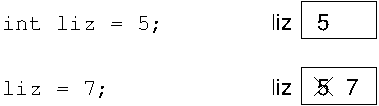
\includegraphics{figs/assign2.pdf}


When there are multiple assignments to a variable, it is especially
important to distinguish between an assignment statement and a
statement of equality.  Because Java uses the {\tt =} symbol for
assignment, it is tempting to interpret a statement like {\tt a = b}
as a statement of equality.  It is not!

First of all, equality is commutative, and assignment is not.
For example, in mathematics if $a = 7$ then $7 = a$.  But in
Java {\tt a = 7;} is a legal assignment statement, and {\tt 7 = a;}
is not.

Furthermore, in mathematics, a statement of equality is true
for all time.  If $a = b$ now, then $a$ will always equal $b$.
In Java, an assignment statement can make two variables equal,
but they don't have to stay that way!

\begin{code}
    int a = 5;
    int b = a;     // a and b are now equal
    a = 3;         // a and b are no longer equal
\end{code}

The third line changes the value of {\tt a} but it does not
change the value of {\tt b}, so they are no longer equal.
In some programming languages a different symbol is used
for assignment, such as {\tt <-} or {\tt :=}, to
avoid this confusion.

Although multiple assignment is frequently useful, you should use it
with caution.  If the values of variables change often, it can make
the code difficult to read and debug.


\section{The {\tt while} statement}
\index{statement!while}
\index{while statement}
\index{iteration}

Computers are often used to automate repetitive tasks.  Repeating
tasks without making errors is something that
computers do well and people do poorly.

We have already seen methods like {\tt countdown} and {\tt factorial}
that use recursion to perform repetition. This process is also called
{\bf iteration}. Java provides language features that make
it easier to write these methods.
In this chapter we are going to look at the {\tt while} statement.
Later on (in Section~\ref{for}) will check out the {\tt for} statement.

Using a {\tt while} statement, we can rewrite {\tt countdown}:

\begin{code}
  public static void countdown(int n) {
    while (n > 0) {
      System.out.println(n);
      n = n-1;
    }
    System.out.println("Blastoff!");
  }
\end{code}

You can almost read a {\tt while} statement like
English.  What this means is, ``While {\tt n} is greater than
zero, print the value of {\tt n} and then reduce
the value of {\tt n} by 1.  When you get to zero, print the
word `Blastoff!'''

More formally, the flow of execution for a {\tt while} statement
is as follows:

\begin{enumerate}

\item Evaluate the condition in parentheses, yielding {\tt true}
or {\tt false}.

\item If the condition is false, exit the {\tt while} statement
and continue execution at the next statement.

\item If the condition is true, execute the statements
between the squiggly-brackets, and then go back to step 1.

\end{enumerate}

This type of flow is called a {\bf loop} because the third step loops
back around to the top.  The statements inside the loop are called
the {\bf body} of the loop.
If the condition is false the
first time through the loop, the statements inside the loop are
never executed.

\index{loop}
\index{loop!body}
\index{loop!infinite}
\index{body!loop}
\index{infinite loop}

The body of the loop should change the value of
one or more variables so that, eventually, the condition becomes
false and the loop terminates.  Otherwise the loop will repeat
forever, which is called an {\bf infinite} loop.  An endless
source of amusement for computer scientists is the observation
that the directions on shampoo, ``Lather, rinse, repeat,'' are
an infinite loop.

In the case of {\tt countdown}, we can prove that the loop
terminates if {\tt n} is positive.
%
In other cases it is not so easy to tell:

\begin{code}
  public static void sequence(int n) {
    while (n != 1) {
      System.out.println(n);
      if (n%2 == 0) {           // n is even
        n = n / 2;
      } else {                  // n is odd
        n = n*3 + 1;
      }
    }
  }
\end{code}

The condition for this loop is {\tt n != 1}, so the loop
will continue until {\tt n} is 1, which will make the condition
false.

At each iteration, the program prints the value of {\tt n} and then
checks whether it is even or odd.  If it is even, the value of
{\tt n} is divided by two.  If it is odd, the value is replaced
by $3n+1$.  For example, if the starting value (the argument passed
to {\tt sequence}) is 3, the resulting sequence is
3, 10, 5, 16, 8, 4, 2, 1.

Since {\tt n} sometimes increases and sometimes decreases, there is no
obvious proof that {\tt n} will ever reach 1, or that the program will
terminate.  For some particular values of {\tt n}, we can prove
termination.  For example, if the starting value is a power of two, then
the value of {\tt n} will be even every time through the loop, until
we get to 1.  The previous example ends with such a sequence,
starting with 16.

Particular values aside, the interesting question is whether
we can prove that this program terminates for {\em all} values of n.
So far, no one has been able to prove it {\em or} disprove it!
For more information, see \url{http://en.wikipedia.org/wiki/Collatz_conjecture}.


\section{Tables}
\index{table}
\index{logarithm}

One of the things loops are good for is generating and printing
tabular data.  For example, before computers were readily
available, people had to calculate logarithms,
sines and cosines, and other common mathematical functions
by hand.

To make that easier, there were books containing long tables
where you could find the values of various functions.
Creating these tables was slow and boring, and the results
were full of errors.

When computers appeared on the scene, one of the initial reactions
was, ``This is great!  We can use the computers to generate the
tables, so there will be no errors.''  That turned out to be true
(mostly), but shortsighted.  Soon thereafter computers were so
pervasive that the tables became obsolete.

Well, almost.  For some operations, computers use tables of values to
get an approximate answer, and then perform computations to improve
the approximation.  In some cases, there have been errors in the
underlying tables, most famously in the table the original Intel
Pentium used to perform floating-point division\footnote{See
  \url{http://en.wikipedia.org/wiki/Pentium_FDIV_bug}.}.

\index{division!floating-point}

Although a ``log table'' is not as useful as it once was, it still
makes a good example of iteration.  The following program prints a
sequence of values in the left column and their logarithms in the
right column:

\begin{code}
    double x = 1.0;
    while (x < 10.0) {
      System.out.println(x + "   " + Math.log(x));
      x = x + 1.0;
    }
\end{code}

The output of this program is

\begin{stdout}
1.0   0.0
2.0   0.6931471805599453
3.0   1.0986122886681098
4.0   1.3862943611198906
5.0   1.6094379124341003
6.0   1.791759469228055
7.0   1.9459101490553132
8.0   2.0794415416798357
9.0   2.1972245773362196
\end{stdout}

Looking at these values, can you tell what base the {\tt log}
method uses?

Since powers of two are important
in computer science, we often want logarithms with
respect to base 2.  To compute them, we can use the formula:

\begin{equation*}
\log_2 x = log_e x / log_e 2
\end{equation*}

Changing the {\tt print} statement to

\begin{code}
      System.out.println(x + "   " + Math.log(x) / Math.log(2.0));
\end{code}

yields

\begin{stdout}
1.0   0.0
2.0   1.0
3.0   1.5849625007211563
4.0   2.0
5.0   2.321928094887362
6.0   2.584962500721156
7.0   2.807354922057604
8.0   3.0
9.0   3.1699250014423126
\end{stdout}

We can see that 1, 2, 4 and 8 are powers of two, because
their logarithms base 2 are round numbers.  If we wanted to find
the logarithms of other powers of two, we could modify the
program like this:

\begin{code}
    double x = 1.0;
    while (x < 100.0) {
      System.out.println(x + "   " + Math.log(x) / Math.log(2.0));
      x = x * 2.0;
    }
\end{code}

Now instead of adding something to {\tt x} each time through
the loop, which yields an arithmetic sequence, we multiply
{\tt x} by something, yielding a {\bf geometric} sequence.
The result is:

\begin{stdout}
1.0   0.0
2.0   1.0
4.0   2.0
8.0   3.0
16.0   4.0
32.0   5.0
64.0   6.0
\end{stdout}

Log tables may not be useful any more, but for computer scientists,
knowing the powers of two is!  When you have an idle
moment, you should memorize the powers of two up to 65536
(that's $2^{16}$).


\section{Two-dimensional tables}
\index{table!two-dimensional}

A two-dimensional table consists of rows and columns that make
it easy to find values at the intersections.  A multiplication
table is a good example.  Let's say you want to print a
multiplication table for the values from 1 to 6.

A good way to start is to write a simple loop that prints
the multiples of 2, all on one line.

\begin{code}
    int i = 1;
    while (i <= 6) {
      System.out.print(2*i + "   ");
      i = i + 1;
    }
    System.out.println("");
\end{code}

The first line initializes a variable named {\tt i}, which is going
to act as a counter, or {\bf loop variable}.  As the loop executes,
the value of {\tt i} increases from 1 to 6; when {\tt i} is 7, the
loop terminates.  Each time through the loop, we print the value {\tt
  2*i} and three spaces.  Since we use {\tt System.out.print},
the output appears on a single line.

\index{loop variable}
\index{variable!loop}

In some environments the
output from {\tt print} gets stored without being displayed until {\tt
println} is invoked.  If the program terminates, and you forget to
invoke {\tt println}, you may never see the stored output.

The output of this program is:

\begin{stdout}
2   4   6   8   10   12
\end{stdout}

So far, so good.  The next step is to {\bf encapsulate} and {\bf
generalize}.


\section{Encapsulation and generalization}
\label{encapsulation}

Encapsulation means taking a piece of code and wrapping it up
in a method, allowing you to take advantage of all the things methods
are good for.  We have seen two examples of encapsulation, when we
wrote {\tt printParity} in Section~\ref{alternative} and {\tt
isSingleDigit} in Section~\ref{boolean}.

Generalization means taking something specific, like printing
multiples of 2, and making it more general, like printing the
multiples of any integer.
\index{encapsulation}
\index{generalization}

Here's a method that encapsulates the loop from the previous
section and generalizes it to print multiples of {\tt n}.

\begin{code}
  public static void printMultiples(int n) {
    int i = 1;
    while (i <= 6) {
      System.out.print(n*i + "   ");
      i = i + 1;
    }
    System.out.println("");
  }
\end{code}

To encapsulate, all I had to do was add the first line,
which declares the name, parameter,
and return type.  To generalize, all I had to do was replace
the value 2 with the parameter {\tt n}.

If I invoke this method with the argument 2, I get the same
output as before.  With argument 3, the output is:

\begin{stdout}
3   6   9   12   15   18
\end{stdout}

and with argument 4, the output is

\begin{stdout}
4   8   12   16   20   24
\end{stdout}

By now you can probably guess how we are going to print a
multiplication table: we'll invoke {\tt printMultiples} repeatedly with
different arguments.  In fact, we are going to use another loop to
iterate through the rows.

\begin{code}
    int i = 1;
    while (i <= 6) {
      printMultiples(i);
      i = i + 1;
    }
\end{code}

First of all, notice how similar this loop is to the one inside {\tt
printMultiples}.  All I did was replace the print statement with a
method invocation.

The output of this program is

\begin{stdout}
1   2   3   4   5   6
2   4   6   8   10   12
3   6   9   12   15   18
4   8   12   16   20   24
5   10   15   20   25   30
6   12   18   24   30   36
\end{stdout}

which is a (slightly sloppy) multiplication table.  If the
sloppiness bothers you, Java provides methods that give you
more control over the format of the output, but I'm not
going to get into that here.


\section{Methods and encapsulation}
\label{methods}
\index{method}
\index{encapsulation}

In Section~\ref{adding_methods} I listed some of the
reasons methods are useful.  Here are several more:

\begin{itemize}

\item By giving a name to a sequence of statements, you make
your program easier to read and debug.

\item Dividing a long program into methods allows you to
separate parts of the program, debug them in isolation, and
then compose them into a whole.

\item Methods facilitate both recursion and iteration.

\item Well-designed methods are often useful for many programs.
Once you write and debug one, you can reuse it.

\end{itemize}

To demonstrate encapsulation again, I'll take the code
from the previous section and wrap it up in a method:

\begin{code}
  public static void printMultTable() {
    int i = 1;
    while (i <= 6) {
      printMultiples(i);
      i = i + 1;
    }
  }
\end{code}

The development process I am demonstrating is called
{\bf encapsulation and generalization}.
You start by adding
code to {\tt main} or another method.  When you get
it working, you extract it and wrap it up in a method.
Then you generalize the method by adding parameters.
\index{program development}
\index{encapsulation}
\index{generalization}

Sometimes you don't know
when you start writing exactly how to divide the program into
methods.  This process lets you design as you go along.


\section{Local variables}
\index{local variable}
\index{variable!local}

You might wonder how we can use the same
variable {\tt i} in both {\tt printMultiples} and {\tt
printMultTable}.  Didn't I say that you can only declare a variable
once?  And doesn't it cause problems when one of the methods changes
the value of the variable?

The answer to both questions is ``no,'' because the {\tt i} in {\tt
printMultiples} and the {\tt i} in {\tt printMultTable} are
{\em not the same variable}.  They have the same name, but
they do not refer to the same storage location, and changing
the value of one has no effect on the other.

Variables declared inside a method definition are
called {\bf local variables} because they only exist inside
the method.  You cannot access a local variable from outside
its ``home'' method, and you are free to have multiple
variables with the same name, as long as they are not in
the same method.

Although it can be confusing, there are good
reasons to reuse names.  For example, it is common to
use the names {\tt i}, {\tt j} and {\tt k} as loop variables.
If you avoid using them in one method just because you
used them somewhere else, you make the program
harder to read.

\index{loop variable}
\index{variable!loop}

\section{More generalization}
\index{generalization}

As another example of generalization, imagine you wanted
a program that would print a multiplication table of any
size, not just the 6x6 table.  You could add a parameter to
{\tt printMultTable}:

\begin{code}
  public static void printMultTable(int high) {
    int i = 1;
    while (i <= high) {
      printMultiples(i);
      i = i + 1;
    }
  }
\end{code}

I replaced the value 6 with the parameter {\tt high}.  If I
invoke {\tt printMultTable} with the argument 7, I get

\begin{stdout}
1   2   3   4   5   6
2   4   6   8   10   12
3   6   9   12   15   18
4   8   12   16   20   24
5   10   15   20   25   30
6   12   18   24   30   36
7   14   21   28   35   42
\end{stdout}

which is fine, except that I probably want the table to
be square (same number of rows and columns), which means
I have to add another parameter to {\tt printMultiples},
to specify how many columns the table should have.

I also call this parameter {\tt high},
demonstrating that different methods can have parameters
with the same name (just like local variables):

\begin{code}
  public static void printMultiples(int n, int high) {
    int i = 1;
    while (i <= high) {
      System.out.print(n*i + "   ");
      i = i + 1;
    }
    System.out.println("");
  }

  public static void printMultTable(int high) {
    int i = 1;
    while (i <= high) {
      printMultiples(i, high);
      i = i + 1;
    }
  }
\end{code}

Notice that when I added a new parameter, I had to change the first
line, and I also had to
change the place where the method is invoked in {\tt printMultTable}.
As expected, this program generates a square 7x7 table:

\begin{stdout}
1   2   3   4   5   6   7
2   4   6   8   10   12   14
3   6   9   12   15   18   21
4   8   12   16   20   24   28
5   10   15   20   25   30   35
6   12   18   24   30   36   42
7   14   21   28   35   42   49
\end{stdout}

When you generalize a method appropriately, you often find
that it has capabilities you did not plan.
For example, you might notice that the multiplication table
is symmetric, because $ab = ba$, so all the entries in the
table appear twice.  You could save ink by printing only
half the table.  To do that, you only have to change one
line of {\tt printMultTable}.  Change

\begin{code}
      printMultiples(i, high);
\end{code}

to

\begin{code}
      printMultiples(i, i);
\end{code}

and you get

\begin{stdout}
1
2   4
3   6   9
4   8   12   16
5   10   15   20   25
6   12   18   24   30   36
7   14   21   28   35   42   49
\end{stdout}

I'll leave it up to you to figure out how it works.


\section{Glossary}

\begin{description}

\item[loop:]  A statement that executes repeatedly while
some condition is satisfied.

\item[infinite loop:]  A loop whose condition is always true.

\item[body:]  The statements inside the loop.

\item[iteration:]  One pass through (execution of) the body
of the loop, including the evaluation of the condition.

\item[encapsulate:]  To divide a large complex program into
components (like methods) and isolate the components from
each other (for example, by using local variables).

\item[local variable:]  A variable that is declared inside
a method and that exists only within that method.  Local variables
cannot be accessed from outside their home method, and do not
interfere with any other methods.

\item[generalize:]  To replace something unnecessarily specific
(like a constant value) with something appropriately general
(like a variable or parameter).  Generalization makes code more
versatile, more likely to be reused, and sometimes even easier
to write.

\item[program development:] A process for writing programs.
  So far we have seen ``incremental development'' and ``encapsulation
  and generalization''.

\index{loop}
\index{infinite loop}
\index{loop!infinite}
\index{iteration}
\index{encapsulation}
\index{generalization}
\index{local variable}
\index{variable!local}
\index{program development}

\end{description}


\section{Exercises}

\begin{exercise}
\label{infloop}

Consider the following code:

\begin{code}
public static void main(String[] args) {
    loop(10);
}

public static void loop(int n) {
    int i = n;
    while (i > 0) {
        System.out.println(i);
        if (i%2 == 0) {
            i = i/2;
        } else {
            i = i+1;
        }
    }
}
\end{code}

\begin{enumerate}

\item Draw a table that shows the value of the variables {\tt i}
and {\tt n} during the execution of {\tt loop}.  The table should
contain one column for each variable and one line for each
iteration.

\item What is the output of this program?

\end{enumerate}
\end{exercise}


\begin{exercise}
Let's say you are given a number, $a$, and you want to find
its square root.  One way to do that is to start with a very
rough guess about the answer, $x_0$, and then improve
the guess using the following formula:

\begin{equation*}
x_1 =(x_0 + a/x_0) / 2
\end{equation*}

For example, if we want to find the square root of 9, and
we start with $x_0 = 6$, then $x_1 =(6 + 9/6) /2 = 15/4 = 3.75$,
which is closer.

We can repeat the procedure, using $x_1$ to calculate $x_2$,
and so on.  In this case, $x_2 = 3.075$ and $x_3 = 3.00091$.
So that is converging very quickly on the right answer(which
is 3).

Write a method called {\tt squareRoot} that takes a {\tt double}
as a parameter and that returns an approximation of the square
root of the parameter, using this technique.  You may not use
{\tt Math.sqrt}.

As your initial guess, you should use $a/2$.  Your method should
iterate until it gets two consecutive estimates that differ by less
than 0.0001; in other words, until the absolute value of $x_n -
x_{n-1}$ is less than 0.0001.  You can use {\tt Math.abs} to calculate
the absolute value.
\end{exercise}


\begin{exercise}
In Exercise~\ref{ex.power} we wrote a recursive version of {\tt
power}, which takes a double {\tt x} and an integer {\tt n} and
returns $x^n$.  Now write an iterative method to perform the same
calculation.
\end{exercise}

\begin{exercise}
Section~\ref{factorial} presents a recursive method
that computes the factorial function.
Write an iterative version of {\tt factorial}.
\end{exercise}

\begin{exercise}
One way to calculate $e^x$ is to use the infinite series expansion

\begin{equation*}
e^x = 1 + x + x^2 / 2! + x^3 / 3! + x^4 / 4! + ...
\end{equation*}

If the loop variable is named {\tt i}, then the $i$th term is
$x^i / i!$.

\begin{enumerate}

\item Write a method called {\tt myexp} that adds up the first {\tt n}
terms of this series.  You can use the {\tt factorial}
method from Section~\ref{factorial} or your iterative version from the
previous exercise.

\item You can make this method much more efficient if you realize that
in each iteration the numerator of the term is the same as its
predecessor multiplied by {\tt x} and the denominator is the same as
its predecessor multiplied by {\tt i}.  Use this observation to
eliminate the use of {\tt Math.pow} and {\tt factorial}, and check
that you still get the same result.

\item Write a method called {\tt check} that takes a single parameter,
{\tt x}, and that prints the values of {\tt x}, {\tt Math.exp(x)} and
{\tt myexp(x)} for various values of {\tt x}.  The output should look
something like:

\begin{stdout}
1.0     2.708333333333333       2.718281828459045
\end{stdout}

%the next line used to use \\ in an attempt to escape the backslash character
%but this doesn't work: \\ produces a newline
%according to the LaTeX symbol list
%http://www.tex.ac.uk/tex-archive/info/symbols/comprehensive/symbols-letter.pdf
%\textbackslash is the actual way to escape a backslash
%(but it seems not to respect the \tt font)
HINT: you can use the String {\tt "\textbackslash t"} to print a tab character
between columns of a table.

\item Vary the number of terms in the series (the second argument
that {\tt check} sends to {\tt myexp}) and see the effect on
the accuracy of the result.  Adjust this value until the estimated
value agrees with the ``correct'' answer when {\tt x} is 1.

\item Write a loop in {\tt main} that invokes {\tt check} with the
values 0.1, 1.0, 10.0, and 100.0.  How does the accuracy of the
result vary as {\tt x} varies?  Compare the number of digits of
agreement rather than the difference between the actual and
estimated values.

\item Add a loop in {\tt main} that checks {\tt myexp} with the values
-0.1, -1.0, -10.0, and -100.0.  Comment on the accuracy.

\end{enumerate}
\end{exercise}


\begin{exercise}
One way to evaluate $\exp(-x^2)$ is to use the infinite series expansion

\begin{equation*}
\exp(-x^2) = 1 - x^2 + x^4/2 - x^6/6 + \ldots
\end{equation*}

In other words, we need to add up a series of terms where the $i$th
term is equal to $(-1)^i x^{2i} / i!$.  Write a method named {\tt gauss}
that takes {\tt x} and {\tt n} as arguments and that returns the sum
of the first {\tt n} terms of the series.  You should not use {\tt
factorial} or {\tt pow}.
\end{exercise}



%\chapter{Strings and things}
\label{chap07}
\label{strings}

\section{Characters}
\index{method!string}
\index{String method}
\index{method!object}
\index{object method}
\index{class!String}

In Java and other object-oriented languages, {\bf objects} are collections
of related data that come with a set of methods.  These methods
operate on the objects, performing computations and sometimes
modifying the object's data.

{\tt Strings} are objects,
so you might ask ``What is the data
contained in a {\tt String} object?''~and~``What are the methods we
can invoke on {\tt String} objects?''
\index{documentation}
%
The components of a {\tt String} object are letters or, more generally,
characters.  Not all characters are letters; some are numbers,
symbols, and other things.  For simplicity I
call them all letters.
%
There are many methods, but I use only a few in this
book.  The rest are documented at
\url{http://download.oracle.com/javase/6/docs/api/java/lang/String.html}.

The first method we will look at is {\tt charAt}, which allows you to
extract letters from a {\tt String}.
% To store the result, we need a new type:
{\tt char} is the variable type that can store
individual characters (as opposed to strings of them).

\index{char}
\index{type!char}
\index{charAt}

{\tt char}s work just like the other types we have seen:

\begin{code}
    char ltr = 'c';
    if (ltr == 'c') {
      System.out.println(ltr);
    }
\end{code}

Character values appear in single quotes, like {\tt 'c'}.  Unlike
string values (which appear in double quotes), character values
can contain only a single letter or symbol.

\index{quote}
\index{double-quote}
\index{value!char}

Here's how the {\tt charAt} method is used:

\begin{code}
    String fruit = "banana";
    char letter = fruit.charAt(1);
    System.out.println(letter);
\end{code}

{\tt fruit.charAt()} means that I am
invoking the {\tt charAt} method on the object named
{\tt fruit}.
I am passing the argument {\tt 1} to this method,
which means that I want to know the first letter of
the string.  The result is a character, which is stored in a
{\tt char} named {\tt letter}.  When I print the value of
{\tt letter}, I get a surprise:

\begin{stdout}
a
\end{stdout}

{\tt a} is not the first letter of {\tt "banana"}.  Unless you are a
computer scientist.  For technical reasons, computer scientists
start counting from zero.  The 0th letter (``zeroeth'') of {\tt
"banana"} is {\tt b}.  The 1th letter (``oneth'') is {\tt a} and the
2th (``twooth'') letter is {\tt n}.

If you want the zereoth letter of a string, you have to pass
0 as an argument:

\begin{code}
    char letter = fruit.charAt(0);
\end{code}


\section{Length}
\index{String!length}
\index{length!String}

The next {\tt String} method we'll look at is {\tt length}, which
returns the number of characters in the string.  For example:

\begin{code}
    int length = fruit.length();
\end{code}

{\tt length} takes no arguments
and returns an integer, in this case 6.  Notice that it is
legal to have a variable with the same name as a method (although
it can be confusing for human readers).

To find the last letter of a string, you might be tempted to
try something like

\begin{code}
    int length = fruit.length();
    char last = fruit.charAt(length);       // WRONG!!
\end{code}

That won't work.  The reason is that there is no 6th letter
in {\tt "banana"}.  Since we started counting at 0, the 6
letters are numbered from 0 to 5.  To get the last character,
you have to subtract 1 from {\tt length}.

\begin{code}
    int length = fruit.length();
    char last = fruit.charAt(length-1);
\end{code}


\section{Traversal}
\label{traverse}
\index{traverse}

A common thing to do with a string is
start at the beginning, select each character in turn, do
some computation with it, and continue until the end.  This pattern
of processing is called a {\bf traversal}.  A natural
way to encode a traversal is with a {\tt while} statement:

\begin{code}
    int index = 0;
    while (index < fruit.length()) {
        char letter = fruit.charAt(index);
        System.out.println(letter);
        index = index + 1;
    }
\end{code}

This loop traverses the string and prints each letter on
a line by itself.  Notice that the condition is
{\tt index < fruit.length()}, which means that when
{\tt index} is equal to the length of the string, the
condition is false and the body of the loop is not executed.
The last character we access is the one with the
index {\tt fruit.length()-1}.

\index{loop variable}
\index{variable!loop}
\index{index}

The name of the loop variable is {\tt index}.  An {\bf
index} is a variable or value used to specify a member of an ordered
set, in this case the string of characters.  The index
indicates (hence the name) which one you want.

\section{Run-time errors}
\label{StringIndexOutOfBounds}
\index{error!run-time}
\index{run-time error}
\index{exception!StringIndexOutOfBounds}

Way back in Section~\ref{run-time} I talked about run-time errors,
which are errors that don't appear until a program has started
running.  In Java run-time errors are called {\bf exceptions}.

You probably haven't seen many run-time errors, because we
haven't been doing many things that can cause one.  Well, now we are.
If you use the {\tt charAt} method and provide an index that is
negative or greater than {\tt length-1}, it {\bf throws} an exception.
You can think of ``throwing'' an exception like throwing
a tantrum.

When that happens, Java prints an error message with
the type of exception and a {\bf stack trace}, which shows the methods
that were running when the exception occurred.  Here is an example:

\begin{code}
public class BadString {

    public static void main(String[] args) {
        processWord("banana");
    }

    public static void processWord(String s) {
        char c = getLastLetter(s);
        System.out.println(c);
    }

    public static char getLastLetter(String s) {
        int index = s.length();         // WRONG!
        char c = s.charAt(index);
        return c;
    }
}
\end{code}

Notice the error in {\tt getLastLetter}: the index of the last
character should be {\tt s.length()-1}.  Here's what you get:

\begin{stdout}
Exception in thread "main" java.lang.StringIndexOutOfBoundsException:
String index out of range: 6
        at java.lang.String.charAt(String.java:694)
        at BadString.getLastLetter(BadString.java:24)
        at BadString.processWord(BadString.java:18)
        at BadString.main(BadString.java:14)
\end{stdout}

Then the program ends.
The stack trace can be hard to read, but it contains a lot of information.


\section{The {\tt indexOf} method}
\index{indexOf}

{\tt indexOf} is the inverse of {\tt charAt}:
{\tt charAt} takes an index and returns the character at that
index;  {\tt indexOf} takes a character and finds the index
where that character appears.

{\tt charAt} fails if the index is out of range, and throws an
exception.  {\tt indexOf} fails if the character does not appear in
the string, and returns the value {\tt -1}.

\begin{code}
    String fruit = "banana";
    int index = fruit.indexOf('a');
\end{code}

This finds the index of the letter {\tt 'a'} in the string.
In this case, the letter appears three times, so it is not
obvious what {\tt indexOf} should do.  According to the
documentation, it returns the index of the {\em first} appearance.

To find subsequent appearances, there is another
version of {\tt indexOf}.  It takes a
second argument that indicates where in the string to start
looking.  For an explanation of this kind
of overloading, see Section~\ref{overloading}.

If we invoke:

\begin{code}
    int index = fruit.indexOf('a', 2);
\end{code}

it starts at the twoeth letter (the first {\tt n}) and finds
the second {\tt a}, which is at index 3.  If the letter happens
to appear at the starting index, the starting index is the
answer.  So

\begin{code}
    int index = fruit.indexOf('a', 5);
\end{code}

returns 5.


\section{Looping and counting}
\label{loopcount}
\index{traverse!counting}
\index{loop!counting}

The following program counts the
number of times the letter {\tt 'a'} appears in a string:

\begin{code}
    String fruit = "banana";
    int length = fruit.length();
    int count = 0;

    int index = 0;
    while (index < length) {
        if (fruit.charAt(index) == 'a') {
            count = count + 1;
        }
        index = index + 1;
    }
    System.out.println(count);
\end{code}

This program demonstrates a common idiom, called a {\bf counter}.  The
variable {\tt count} is initialized to zero and then incremented each
time we find an {\tt 'a'}. To {\bf increment} is to increase by one;
it is the opposite of {\bf decrement}.
%, and unrelated to {\bf excrement}, which is a noun
When we exit the loop, {\tt count}
contains the result: the total number of a's.
\index{counter}
\index{increment}
\index{decrement}


\section{Increment and decrement operators}
\index{operator!increment}
\index{operator!decrement}

Incrementing and decrementing are such common operations that
Java provides special operators for them.  The {\tt ++}
operator adds one to the current value of an {\tt int} or
{\tt char}.  {\tt --} subtracts one.  Neither operator works
on {\tt double}s, {\tt boolean}s or {\tt String}s.

Technically, it is legal to increment a variable and use it
in an expression at the same time.  For example, you might see
something like:

\begin{code}
    System.out.println(i++);
\end{code}

Looking at this, it is not clear whether the increment will
take effect before or after the value is printed.  Because
expressions like this tend to be confusing, I discourage
you from using them.  In fact, to discourage you even more,
I'm not going to tell you what the result is.  If you really
want to know, you can try it.

Using the increment operators, we can rewrite the letter-counter:

\begin{code}
    int index = 0;
    while (index < length) {
      if (fruit.charAt(index) == 'a') {
        count++;
      }
      index++;
    }
\end{code}

It is a common error to write something like

\begin{code}
    index = index++;             // WRONG!!
\end{code}

Unfortunately, this is syntactically legal, so the compiler
will not warn you.  The effect of this statement is to leave
the value of {\tt index} unchanged.  This is often a difficult
bug to track down.

Remember, you can write {\tt index = index+1}, or you
can write {\tt index++}, but you shouldn't mix them.

% \section{Character arithmetic}
% \index{char}
% \index{type!char}
% \index{operator!char}
% \index{arithmetic!char}

% It may seem odd, but you can do arithmetic with characters.
% If you have a variable named {\tt letter} that contains a character,
% then {\tt letter - 'a'} will tell you where in the alphabet it appears
%(keeping in mind that 'a' is the zeroeth letter of the alphabet and
% 'z' is the 25th).

% This sort of thing is useful for converting between the characters
% that contain numbers, like '0', '1' and '2', and the corresponding
% integers.  They are not the same thing.  For example, if you try this

% \begin{code}
%     char letter = '3';
%     int x =(int) letter;
%     System.out.println(x);
% \end{code}
% %
% you might expect the value 3, but depending on your environment,
% you might get 51, which is the ASCII code that is used to
% represent the character '3', or you might get something else
% altogether.  To convert '3' to the corresponding integer value
% you can subtract '0':

% \begin{code}
%     int x =(int)(letter - '0');
% \end{code}
% %
% Technically, in both of these examples the typecast({\tt(int)}) is
% unnecessary, since Java will convert type {\tt char} to type {\tt int}
% automatically.  I included the typecasts to emphasize the difference
% between the types, and because I'm a stickler about that sort of
% thing.

% Since this conversion can be a little ugly, it is preferable to use
% the {\tt digit} method in the {\tt Character} class.  For example:

% \begin{code}
%     int x = Character.digit(letter, 10);
% \end{code}
% %
% converts {\tt letter} to the corresponding digit, interpreting
% it as a base 10 number.

% Another use for character arithmetic is to loop through the letters of
% the alphabet in order.  For example, in Robert McCloskey's book {\em
% Make Way for Ducklings}, the names of the ducklings form an
% abecedarian series: Jack, Kack, Lack, Mack, Nack, Ouack, Pack and
% Quack.  Here is a loop that prints these names in order:

% \begin{code}
%     char letter = 'J';
%     while (letter <= 'Q') {
 %      System.out.println(letter + "ack");
 %      letter++;
%     }
% \end{code}
%
% Notice that in addition to the arithmetic operators, we can also
% use the conditional operators on characters.  The output of this
% program is:

% \begin{stdout}
% Jack
% Kack
% Lack
% Mack
% Nack
% Oack
% Pack
% Qack
% \end{stdout}
% %
% Of course, that's not quite right because I've misspelled ``Ouack''
% and ``Quack.''  As an exercise, modify the program to correct
% this error.


\section{{\tt String}s are immutable}
\label{immutable}
\index{class!String}
\index{immutable}
\index{String}
\index{toUpperCase}
\index{toLowerCase}

As you read the documentation of the {\tt String} methods, you
might notice {\tt toUpperCase} and {\tt toLowerCase}.  These
methods are often a source of confusion, because it sounds
like they have the effect of changing (or mutating) an
existing string.  Actually, neither these methods nor any
others can change a string, because strings are {\bf immutable}.

When you invoke {\tt toUpperCase} on a {\tt String}, you get a
{\em new} {\tt String} as a return value.  For example:

\begin{code}
    String name = "Alan Turing";
    String upperName = name.toUpperCase();
\end{code}

After the second line is executed, {\tt upperName} contains
the value {\tt "ALAN TURING"}, but {\tt name} still contains
{\tt "Alan Turing"}.
\index{Turing, Alan}


\section{{\tt String}s are incomparable}
\label{incomparable}
\index{class!String}
\index{comparison!String}
\index{String}
\index{equals}
\index{compareTo}

It is often necessary to compare strings to see if they are the same,
or to see which comes first in alphabetical order.  It would be
nice if we could use the comparison operators, like {\tt ==} and
{\tt >}, but we can't.

To compare {\tt String}s, we have to use the {\tt equals}
and {\tt compareTo} methods.  For example:

\begin{code}
    String name1 = "Alan Turing";
    String name2 = "Ada Lovelace";

    if (name1.equals (name2)) {
      System.out.println("The names are the same.");
    }

    int flag = name1.compareTo (name2);
    if (flag == 0) {
      System.out.println("The names are the same.");
    } else if (flag < 0) {
      System.out.println("name1 comes before name2.");
    } else if (flag > 0) {
      System.out.println("name2 comes before name1.");
    }
\end{code}

The syntax here is a little weird.  To compare two {\tt String}s,
you have to invoke a method on one of them and pass the other as an
argument.

The return value from {\tt equals} is straightforward enough;
{\tt true} if the strings contain the same characters, and
{\tt false} otherwise.

The return value from {\tt compareTo} is a weird, too.  It is
the difference between the first characters in the strings
that differ.  If the strings are equal, it is 0.  If the
first string (the one on which the method is invoked) comes
first in the alphabet, the difference is negative.  Otherwise,
the difference is positive.  In this case the return value
is positive 8, because the second letter of ``Ada'' comes
before the second letter of ``Alan'' by 8 letters.

Just for completeness, I should admit that it is {\em legal}, but very
seldom {\em correct}, to use the {\tt ==} operator with {\tt String}s.
I explain why in Section~\ref{equivalence}; for now, don't do it.


\section{Glossary}

\begin{description}

\item[object:] A collection of related data that comes with a set of
methods that operate on it.  The objects we have used so far are
{\tt String}s, Bugs, Rocks, and the other GridWorld objects.

\item[index:]  A variable or value used to select one of the
members of an ordered set, like a character from a string.

\item[exception:] A run-time error.
\index{exception}
\index{run-time error}

\item[throw:] Cause an exception.

\item[stack trace:] A report that shows the state of a program
when an exception occurs.

\item[prototype:]  The first line of a method, which specifies
the name, parameters and return type.

\item[traverse:]  To iterate through all the elements of a set
performing a similar operation on each.

\item[counter:]  A variable used to count something, usually
initialized to zero and then incremented.

\item[increment:]  Increase the value of a variable by one.
The increment operator in Java is {\tt ++}.

\item[decrement:]  Decrease the value of a variable by one.
The decrement operator in Java is {\tt --}.


\index{object}
\index{index}
\index{traverse}
\index{counter}
\index{increment}
\index{decrement}

\end{description}


\section{Exercises}

\begin{exercise}
Write a method that takes a {\tt String}
as an argument and that prints the letters backwards all on
one line.
\end{exercise}

\begin{exercise}
Read the stack trace in Section~\ref{StringIndexOutOfBounds}
and answer these questions:

\begin{itemize}

\item What kind of Exception occurred, and what package is it defined
in?

\item What is the value of the index that caused the exception?

\item What method threw the exception, and where is
that method defined?

\item What method invoked {\tt charAt}?

\item In {\tt BadString.java}, what is the line number where {\tt charAt}
was invoked?

\end{itemize}

\end{exercise}

\begin{exercise}

Encapsulate the code in Section~\ref{loopcount} in a method named
{\tt countLetters}, and generalize it so that it accepts the
string and the letter as arguments.
\index{encapsulation}
\index{generalization}

Then rewrite the method so that it uses
{\tt indexOf} to locate the a's, rather than checking
the characters one by one.

\end{exercise}

\begin{exercise}
The purpose of this exercise is to review encapsulation
and generalization.

\begin{enumerate}

\item Encapsulate the following code fragment, transforming it
into a method that takes a String as an argument and that
returns the final value of {\tt count}.

\item In a sentence or two, describe what the resulting method does
(without getting into the details of how).

\item Now that you have generalized the code
so that it works on any String, what could you do to
generalize it more?

\end{enumerate}

\begin{code}
    String s = "((3 + 7) * 2)";
    int len = s.length();

    int i = 0;
    int count = 0;

    while (i < len) {
        char c = s.charAt(i);

        if (c == '(') {
           count = count + 1;
        } else if (c == ')') {
           count = count - 1;
        }
        i = i + 1;
    }

    System.out.println(count);
\end{code}
\end{exercise}


\begin{exercise}

The point of this exercise is to explore Java types
and fill in some of the details that aren't covered
in the chapter.

\begin{enumerate}

\item Create a new program named {\tt Test.java} and write
a {\tt main} method that contains
expressions that combine
various types using the {\tt +} operator.  For example, what
happens when you ``add'' a {\tt String} and a {\tt char}?
Does it perform addition or concatenation?   What is the type
of the result? (How can you determine the type of the result?)

\item Make a bigger copy of the following table and fill it in.  At the
intersection of each pair of types, you should indicate whether it is
legal to use the {\tt +} operator with these types, what operation is
performed (addition or concatenation), and what the type of the result
is.

\begin{tabular}{|l|l|l|l|l|} \hline
        &  boolean  &  char  &  int  &  String \\ \hline
boolean &           &        &       &         \\ \hline
char    &           &        &       &         \\ \hline
int     &           &        &       &         \\ \hline
String  &           &        &       &         \\ \hline
\end{tabular}

\item Think about some of the choices the designers of Java
made when they filled in this table.  How many of the entries
seem unavoidable, as if there were no other choice?
How many seem like arbitrary choices from several equally
reasonable possibilities?  How many seem problematic?

\item Here's a puzzler: normally, the statement {\tt x++} is exactly
  equivalent to {\tt x = x + 1}.  But if {\tt x} is a {\tt char}, it's
  not!  In that case, {\tt x++} is legal, but {\tt x = x + 1} causes
  an error.  Try it out and see what the error message is, then see if
  you can figure out what is going on.

\end{enumerate}
\end{exercise}


\begin{exercise}

What is the output of this program?  Describe in a sentence
what {\tt mystery} does (not how it works).

\begin{code}
public class Mystery {

    public static String mystery(String s) {
        int i = s.length() - 1;
        String total = "";

        while (i >= 0 ) {
            char ch = s.charAt(i);
            System.out.println(i + "     " + ch);

            total = total + ch;
            i--;
        }
        return total;
    }

    public static void main(String[] args) {
        System.out.println(mystery("Allen"));
    }
}
\end{code}

\end{exercise}


\begin{exercise}
A friend of yours shows you the following method and
explains that if {\tt number} is any two-digit number, the program
will output the number backwards.  He claims that if {\tt number} is
17, the method will output {\tt 71}.

Is he right?  If not, explain what the program actually does and
modify it so that it does the right thing.

\begin{code}
     int number = 17;
     int lastDigit = number%10;
     int firstDigit = number/10;
     System.out.println(lastDigit + firstDigit);
\end{code}

\end{exercise}

\begin{exercise}
What is the output of the following program?

\begin{code}
public class Enigma {

    public static void enigma(int x) {
        if (x == 0) {
            return;
        } else {
            enigma(x/2);
        }

        System.out.print(x%2);
    }

    public static void main(String[] args) {
        enigma(5);
        System.out.println("");
    }
}
\end{code}

Explain in 4-5 words what the method {\tt enigma} really does.
\end{exercise}


\begin{exercise}
\label{palindrome}

\begin{enumerate}

\item Create a new program named {\tt Palindrome.java}.

\item Write a method named {\tt first}
that takes a String and returns the first letter, and one named
{\tt last} that returns the last letter.

\item Write a method named {\tt middle} that takes a String and
returns a substring that contains everything {\em except} the
first and last characters.

Hint: read the documentation of the {\tt substring} method in
the {\tt String} class.
Run a few tests to make sure you understand how {\tt substring} works
before you try to write {\tt middle}.

What happens if you invoke {\tt middle} on a string that has only
two letters?  One letter?  No letters?

\item The usual definition of a palindrome is a word that reads the
same both forward and backward, like ``otto'' and
``palindromeemordnilap.''  An alternative way to define a property
like this is to specify a way of testing for the property.  For
example, we might say, ``a single letter is a palindrome, and a
two-letter word is a palindrome if the letters are the same, and
any other word is a palindrome if
the first letter is the same as the
last and the middle is a palindrome.''

Write a recursive method named {\tt isPalindrome} that takes
a {\tt String} and that returns a boolean indicating whether the
word is a palindrome or not.

\item Once you have a working palindrome checker, look for ways
to simplify it by reducing the number of conditions you check.
Hint: it might be useful to adopt the definition that the empty
string is a palindrome.

\item On a piece of paper, figure out a strategy for checking
palindromes iteratively.  There are several possible approaches,
so make sure you have a solid plan before you start writing code.

\item Implement your strategy in a method called {\tt isPalindromeIter}.

\item Optional: Appendix~\ref{javaio} provides code for reading a list
of words from a file.  Read a list of words and print the palindromes.

\end{enumerate}
\end{exercise}


\begin{exercise}
\label{abecedarian}

A word is said to be ``abecedarian'' if the letters in the
word appear in alphabetical order.  For example, the following
are all 6-letter English abecedarian words.

\begin {quote}
abdest, acknow, acorsy, adempt, adipsy, agnosy, befist, behint,
beknow, bijoux, biopsy, cestuy, chintz, deflux, dehors, dehort,
deinos, diluvy, dimpsy
\end{quote}

\begin{enumerate}

\item Describe a process for checking whether a given word (String)
is abecedarian, assuming that the word contains only lower-case
letters.  Your process can be iterative or recursive.

\item Implement your process in a method called {\tt isAbecedarian}.

\end{enumerate}
\end{exercise}


\begin{exercise}
\label{dupledrome}
A dupledrome is a word that contains only double letters,
like ``llaammaa'' or ``ssaabb''.  I conjecture that there
are no dupledromes in common English use.  To test that
conjecture, I would like a program that reads
words from the dictionary one at a time and checks them for
dupledromity.

Write a method called {\tt isDupledrome} that takes a String
and returns a boolean indicating whether the word is a dupledrome.
\end{exercise}



\begin{exercise}
\begin{enumerate}

\item The Captain Crunch decoder ring works by taking each letter in a
string and adding 13 to it.  For example, 'a' becomes 'n' and 'b'
becomes 'o'.  The letters ``wrap around'' at the end, so 'z' becomes
'm'.

Write a method that takes a String and that returns a new String
containing the encoded version.  You should assume that the String
contains upper and lower case letters, and spaces, but no other
punctuation.  Lower case letters should be tranformed into other lower
case letters; upper into upper.  You should not encode the spaces.

\item Generalize the Captain Crunch method so that instead of adding
13 to the letters, it adds any given amount.  Now you should be able
to encode things by adding 13 and decode them by adding -13.  Try it.

\end{enumerate}
\end{exercise}


\begin{exercise}

If you did the GridWorld exercises in Chapter~\ref{gridworld}, you
might enjoy this exercise.  The goal is to use trigonometry to get the
Bugs to chase each other.

Make a copy of {\tt BugRunner.java} named {\tt ChaseRunner.java} and
import it into your development environment.  Before you change
anything, check that you can compile and run it.

\begin{itemize}

\item Create two Bugs, one red and one blue.

\item Write a method called {\tt distance} that takes two Bugs
and computes the distance between them.  Remember that you can
get the x-coordinate of a Bug like this:

\begin{code}
    int x = bug.getLocation().getCol();
\end{code}

\item Write a method called {\tt turnToward} that takes two
Bugs and turns one to face the other.  HINT: use {\tt Math.atan2},
but remember that the result is in radians, so you have to
convert to degrees.  Also, for Bugs, 0 degress is North, not East.

\item Write a method called {\tt moveToward} that takes two
Bugs, turns the first to face the second, and then moves the
first one, if it can.

\item Write a method called {\tt moveBugs} that takes two Bugs
and an integer {\tt n}, and moves each Bug toward the other {\tt n}
times.  You can write this method recursively, or use a while loop.

\item Test each of your methods as you develop them.  When they are
  all working, look for opportunities to improve them.  For example,
  if you have redundant code in {\tt distance} and {\tt turnToward},
  you could encapsulate the repeated code in a method.

\end{itemize}

\end{exercise}





%\chapter{Mutable objects}
\label{chap08}
\label{objects}
\index{object}


%\section{{\tt Point}s and {\tt Rectangle}s}
\index{String}
\index{type!String}

{\tt String}s are objects, but they are atypical objects
because

\begin{itemize}

\item They are immutable.

\item They have no attributes.

\item You don't have to use {\tt new} to create one.

\end{itemize}

In this chapter, we use two objects from Java libraries,
 {\tt Point} and {\tt Rectangle}.
But first, I want to make it clear that these points
and rectangles are not graphical objects that appear on the
screen.  They are values that contain data, just like {\tt int}s
and {\tt double}s.  Like other values, they are used internally
to perform computations.


%\index{AWT}
%\index{Abstract Window Toolkit|see {AWT}}

%, and {\tt java.awt}, the {\bf Abstract Window Toolkit} (AWT), which contains classes for windows, buttons, graphics, etc.

% {\tt Point} and {\tt Rectangle} are in the {\tt java.awt} package, so to import them like this:


\section{{\tt Point} objects}
\index{Point}
\index{class!Point}

A point is two numbers (coordinates)
that we treat collectively as a single object.  In mathematical
notation, points are often written in parentheses, with a comma
separating the coordinates.  For example, $(0, 0)$ indicates
the origin, and $(x, y)$ indicates the point $x$ units to the
right and $y$ units up from the origin.

\index{new}
\index{statement!new}

In Java, a point is represented by a {\tt Point} object.  To
create a new point, you have to use {\tt new}:

\begin{code}
    Point blank;
    blank = new Point(3, 4);
\end{code}

The first line is a conventional variable declaration: {\tt blank}
has type {\tt Point}.  The second line invokes {\tt new}, specifies
the type of the new object, and provides arguments.  The arguments are
the coordinates of the new point, $(3, 4)$.

\index{declaration}
\index{statement!declaration}
\index{reference}
\index{state diagram}
\index{state}

The result of {\tt new} is a {\bf reference} to the new
point, so {\tt blank} contains a reference to the
newly-created object.  There is a standard way to diagram this
assignment, shown in the figure.


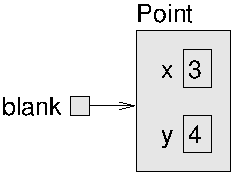
\includegraphics{figs/reference.pdf}


As usual, the name of the variable {\tt blank} appears outside the box
and its value appears inside the box.  In this case, that value is a
reference, which is shown graphically with an arrow.  The
arrow points to the object we're referring to.

The big box shows the newly-created object with the two values
in it.  The names {\tt x} and {\tt y} are the names of the {\bf
instance variables}.

Taken together, all the variables, values, and objects in a
program are called the {\bf state}.  Diagrams like this that
show the state of the program are called {\bf state diagrams}.
As the program runs, the state changes, so you should think
of a state diagram as a snapshot of a particular point in the
execution.


\section{Instance variables}
\index{variable!instance}
\index{instance variable}

The pieces of data that make up an object are called instance
variables because each object, which is an {\bf instance} of its
type, has its own copy of the instance variables.

It's like the glove compartment of a car.  Each car is an instance
of the type ``car,'' and each car has its own glove compartment.  If
you ask me to get something from the glove compartment of your car,
you have to tell me which car is yours.

\index{dot notation}

Similarly, if you want to read a value from an instance variable, you
have to specify the object you want to get it from.  In Java this is
done using ``dot notation.''

\begin{code}
    int x = blank.x;
\end{code}

The expression {\tt blank.x} means ``go to the object {\tt blank}
refers to, and get the value of {\tt x}.''  In this case we assign
that value to a local variable named {\tt x}.  There is no
conflict between the local variable named {\tt x} and the instance
variable named {\tt x}.  The purpose of dot notation is to identify
{\em which} variable you are referring to unambiguously.

You can use dot notation as part of any Java expression, so the
following are legal.

\begin{code}
    System.out.println(blank.x + ", " + blank.y);
    int sum = blank.x * blank.x + blank.y * blank.y;
\end{code}

The first line prints {\tt 3, 4}; the second line calculates
the value 25.

\section{Objects as parameters}
\index{parameter}
\index{object!as parameter}

You can pass objects as parameters in the usual way.  For
example:

\begin{code}
  public static void printPoint(Point p) {
    System.out.println("(" + p.x + ", " + p.y + ")");
  }
\end{code}

This method takes a point as an argument and prints it in
the standard format.  If you invoke {\tt printPoint(blank)},
it prints {\tt(3, 4)}.  Actually, Java already has a
method for printing {\tt Points}.  If you invoke
{\tt System.out.println(blank)}, you get

\begin{code}
java.awt.Point[x=3,y=4]
\end{code}

This is a standard format Java uses for printing objects.  It prints
the name of the type, followed by the names and values of the instance
variables.

As a second example, we can rewrite the {\tt distance} method from
Section~\ref{distance} so that it takes two {\tt Point}s as parameters
instead of four {\tt double}s.

\begin{code}
  public static double distance(Point p1, Point p2) {
    double dx = (double)(p2.x - p1.x);
    double dy = (double)(p2.y - p1.y);
    return Math.sqrt(dx*dx + dy*dy);
  }
\end{code}

The typecasts are not really necessary; I added them as a
reminder that the instance variables in a {\tt Point} are integers.


\section{Rectangles}
\index{Rectangle}
\index{class!Rectangle}

{\tt Rectangle}s are similar to points, except that they have four
instance variables: {\tt x}, {\tt y}, {\tt width} and {\tt
height}.  Other than that, everything is pretty much the same.

This example
creates a {\tt Rectangle} object and makes {\tt box} refer to it.

\begin{code}
    Rectangle box = new Rectangle(0, 0, 100, 200);
\end{code}

This figure shows the effect of this assignment.


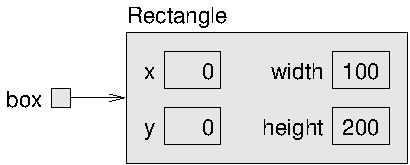
\includegraphics{figs/rectangle.pdf}

If you print {\tt box}, you get

\begin{code}
java.awt.Rectangle[x=0,y=0,width=100,height=200]
\end{code}

Again, this is the result of a Java method that knows how
to print {\tt Rectangle} objects.


\section{Objects as return types}
\index{object!as return type}
\index{return}
\index{statement!return}

You can write methods that return objects.  For example,
{\tt findCenter} takes a {\tt Rectangle} as an argument and
returns a {\tt Point} that contains the coordinates of the
center of the {\tt Rectangle}:

\begin{code}
  public static Point findCenter(Rectangle box) {
    int x = box.x + box.width/2;
    int y = box.y + box.height/2;
    return new Point(x, y);
  }
\end{code}

Notice that you can use {\tt new} to create a new object,
and then immediately use the result as the return value.


\section{Objects are mutable}
\index{object!mutable}
\index{mutable}

You can change the contents of an object by making an assignment
to one of its instance variables.  For example, to ``move''
a rectangle without changing its size, you can modify the
{\tt x} and {\tt y} values:

\begin{code}
    box.x = box.x + 50;
    box.y = box.y + 100;
\end{code}

The result is shown in the figure:


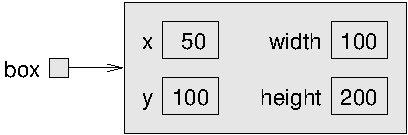
\includegraphics{figs/rectangle2.pdf}


\index{encapsulation}
\index{generalization}

We can encapsulate this code in a method and
generalize it to move the rectangle by any amount:

\begin{code}
  public static void moveRect(Rectangle box, int dx, int dy) {
    box.x = box.x + dx;
    box.y = box.y + dy;
  }
\end{code}

The variables {\tt dx} and {\tt dy} indicate how far to move the
rectangle in each direction.  Invoking this method has the effect of
modifying the {\tt Rectangle} that is passed as an argument.

\begin{code}
    Rectangle box = new Rectangle(0, 0, 100, 200);
    moveRect(box, 50, 100);
    System.out.println(box);
\end{code}

prints {\tt java.awt.Rectangle[x=50,y=100,width=100,height=200]}.

Modifying objects by passing them as arguments to methods can be
useful, but it can also make debugging more difficult because it is
not always clear which method invocations do or do not modify their
arguments.  Later, I discuss some pros and cons of this
programming style.

Java provides methods that operate on Points and Rectangles.  You can
read the documentation at
\url{http://download.oracle.com/javase/6/docs/api/java/awt/Point.html}
and
\url{http://download.oracle.com/javase/6/docs/api/java/awt/Rectangle.html}.

For example, {\tt translate} has the same effect as {\tt moveRect},
but instead of passing the Rectangle as an argument, you use dot
notation:

\begin{code}
    box.translate(50, 100);
\end{code}

%The effect is the same.


\section{Aliasing}
\label{aliasing}
\index{aliasing}
\index{reference}

Remember that when you assign an object to a variable, you
are assigning a {\em reference} to an object.  It is possible to have
multiple variables that refer to the same object.  For example,
this code:

\begin{code}
    Rectangle box1 = new Rectangle(0, 0, 100, 200);
    Rectangle box2 = box1;
\end{code}

generates a state diagram that looks like this:


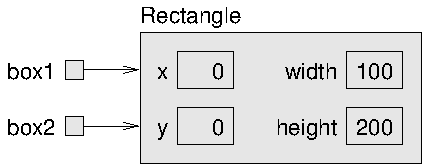
\includegraphics{figs/aliasing.pdf}


{\tt box1} and {\tt box2} refer to the same object.
In other words, this object has two names, {\tt box1} and {\tt box2}.
When a person uses two names, it's called {\bf aliasing}.  Same thing
with objects.

When two variables are aliased, any changes that affect one
variable also affect the other.  For example:

\begin{code}
    System.out.println(box2.width);
    box1.grow(50, 50);
    System.out.println(box2.width);
\end{code}

The first line prints {\tt 100}, which is the width of the
{\tt Rectangle} referred to by {\tt box2}.  The second
line invokes the {\tt grow} method on {\tt box1}, which
expands the {\tt Rectangle} by 50 pixels in every direction
(see the documentation for more details).  The effect
is shown in the figure:


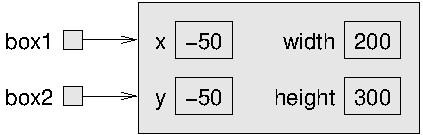
\includegraphics{figs/aliasing2.pdf}


Whatever changes are
made to {\tt box1} also apply to {\tt box2}.  Thus, the
value printed by the third line is {\tt 200}, the width of
the expanded rectangle. (As an aside, it is perfectly legal
for the coordinates of a {\tt Rectangle} to be negative.)

As you can tell even from this simple example, code that
involves aliasing can get confusing fast, and can be
difficult to debug.  In general, aliasing should be avoided
or used with care.


\section{{\tt null}}
\index{null}

When you create an object variable, remember that you are
creating a {\em reference} to an object.  Until you make
the variable point to an object, the value of the variable
is {\tt null}.  {\tt null} is a special value (and
a Java keyword) that means ``no object.''

The declaration {\tt Point blank;} is equivalent to this
initialization

\begin{code}
    Point blank = null;
\end{code}

and is shown in the following state diagram:



\includegraphics{figs/reference2.pdf}


The value {\tt null} is represented by a small square with no arrow.

\index{exception!NullPointer}
\index{run-time error}

If you try to use a null object, either by accessing an instance
variable or invoking a method, Java throws a {\tt
NullPointerException}, prints an error message
and terminates the program.

\begin{code}
    Point blank = null;
    int x = blank.x;              // NullPointerException
    blank.translate(50, 50);      // NullPointerException
\end{code}

On the other hand, it is legal to pass a null object as an argument or
receive one as a return value.  In fact, it is common to do so, for
example to represent an empty set or indicate an error condition.


\section{Garbage collection}
\index{garbage collection}

In Section~\ref{aliasing} we talked about what happens when
more than one variable refers to the same object.  What happens
when {\em no} variable refers to an object?  For example:

\begin{code}
    Point blank = new Point(3, 4);
    blank = null;
\end{code}

The first line creates a new {\tt Point} object and makes
{\tt blank} refer to it.  The second line changes {\tt blank}
so that instead of referring to the object, it refers to
nothing (the null object).


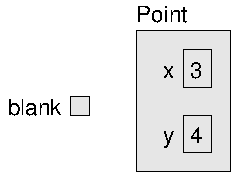
\includegraphics{figs/reference3.pdf}


If no one refers to an object, then no one can read or write any of
its values, or invoke a method on it.  In effect, it ceases to exist.
We could keep the object in memory, but it would only waste space, so
periodically as your program runs, the system looks for stranded
objects and reclaims them, in a process called {\bf garbage
collection}.  Later, the memory space occupied by the object will
be available to be used as part of a new object.

You don't have to do anything to make garbage collection happen,
and in general you will not be aware of it.  But you
should know that it periodically runs in the background.


\section{Glossary}

\begin{description}

\item[AWT:]  The Abstract Window Toolkit, one of the biggest
and commonly-used Java packages.

\item[instance:]  An example from a category.  My cat is an
instance of the category ``feline things.''  Every object is
an instance of some class.

\item[instance variable:]  One of the named data items that make
up an object.  Each object (instance) has its own copy of
the instance variables for its class.

\item[reference:]  A value that indicates an object.  In a
state diagram, a reference appears as an arrow.

\item[aliasing:] The condition when two or more variables refer
to the same object.

\item[garbage collection:]  The process of finding objects that
have no references and reclaiming their storage space.

\item[state:] A complete description of all the variables and
objects and their values, at a given point during the execution
of a program.

\item[state diagram:] A snapshot of the state of a program, shown
graphically.

\index{instance}
\index{instance variable}
\index{reference}
\index{aliasing}
\index{garbage collection}
\index{state}
\index{state diagram}

\end{description}


\section{Exercises}

\begin{exercise}
\begin{enumerate}

\item For the following program, draw a stack diagram showing the
local variables and parameters of {\tt main} and {\tt riddle}, and show
any objects those variables refer to.

\item What is the output of this program?

\end{enumerate}

\begin{code}
public static void main(String[] args)
{
    int x = 5;
    Point blank = new Point(1, 2);

    System.out.println(riddle(x, blank));
    System.out.println(x);
    System.out.println(blank.x);
    System.out.println(blank.y);
}

public static int riddle(int x, Point p)
{
    x = x + 7;
    return x + p.x + p.y;
}
\end{code}

The point of this exercise is to make sure you understand the
mechanism for passing Objects as parameters.
\end{exercise}


\begin{exercise}
\begin{enumerate}

\item For the following program, draw a stack diagram showing the
state of the program just before {\tt distance} returns.  Include all
variables and parameters and the objects those variables refer to.

\item What is the output of this program?

\end{enumerate}

\begin{code}
public static double distance(Point p1, Point p2) {
    int dx = p1.x - p2.x;
    int dy = p1.y - p2.y;
    return Math.sqrt(dx*dx + dy*dy);
}

public static Point findCenter(Rectangle box) {
    int x = box.x + box.width/2;
    int y = box.y + box.height/2;
    return new Point(x, y);
}

public static void main(String[] args) {
    Point blank = new Point(5, 8);

    Rectangle rect = new Rectangle(0, 2, 4, 4);
    Point center = findCenter(rect);

    double dist = distance(center, blank);

    System.out.println(dist);
}
\end{code}

\end{exercise}



\begin{exercise}
The method {\tt grow} is part of the {\tt Rectangle} class.  Read the
documentation at
\url{http://download.oracle.com/javase/6/docs/api/java/awt/Rectangle.html#grow(int, int)}.

\begin{enumerate}

\item What is the output of the following program?

\item Draw a state diagram that shows the state of the
program just before the end of {\tt main}.
Include all local variables and the objects
they refer to.

\item At the end of {\tt main}, are {\tt p1} and
{\tt p2} aliased?  Why or why not?

\end{enumerate}

\begin{code}
public static void printPoint(Point p) {
    System.out.println("(" + p.x + ", " + p.y + ")");
}

public static Point findCenter(Rectangle box) {
    int x = box.x + box.width/2;
    int y = box.y + box.height/2;
    return new Point(x, y);
}

public static void main(String[] args) {

    Rectangle box1 = new Rectangle(2, 4, 7, 9);
    Point p1 = findCenter(box1);
    printPoint(p1);

    box1.grow(1, 1);
    Point p2 = findCenter(box1);
    printPoint(p2);
}
\end{code}

\end{exercise}


\begin{exercise}
\label{ex.biginteger}
You might be sick of the factorial
method by now, but we're going to do one more version.

\begin{enumerate}

\item Create a new program called {\tt Big.java} and
write an iterative version of {\tt factorial}.

\item Print a table of the integers from 0 to 30 along with their
factorials.  At some point around 15, you will probably see
that the answers are not right any more.  Why not?

\item BigIntegers are Java objects that can represent arbitrarily big
  integers.  There is no upper bound except the limitations of memory
  size and processing speed.  Read the documentation of BigIntegers at
  \url{http://download.oracle.com/javase/6/docs/api/java/math/BigInteger.html}.

\item To use BigIntegers, you have to add {\tt import
java.math.BigInteger} to the beginning of your program.

\item There are several ways to create a
BigInteger, but the one I recommend uses {\tt valueOf}.
The following code converts an integer to a {\tt BigInteger}:

\begin{code}
    int x = 17;
    BigInteger big = BigInteger.valueOf(x);
\end{code}

Type in this code and try it out.  Try printing a BigInteger.

\item Because BigIntegers are not primitive types,
the usual math operators don't work.  Instead we
have to use methods like {\tt add}.  To
add two BigIntegers, invoke {\tt add} on one
and pass the other as an argument.  For example:

\begin{code}
    BigInteger small = BigInteger.valueOf(17);
    BigInteger big = BigInteger.valueOf(1700000000);
    BigInteger total = small.add(big);
\end{code}

Try out some of the other methods, like {\tt multiply} and
{\tt pow}.

\item Convert {\tt factorial} so that it performs its calculation
using BigIntegers and returns a BigInteger as a result.
You can leave the parameter alone---it will still be an integer.

\item Try printing the table again with your modified factorial
method.  Is it correct up to 30?  How high can you make it go?  I
calculated the factorial of all the numbers from 0 to 999, but my
machine is pretty slow, so it took a while.  The last number, 999!,
has 2565 digits.

\end{enumerate}
\end{exercise}

\begin{exercise}
Many encryption techniques depend on the
ability to raise large integers to an integer power.  Here is a
method that implements a (reasonably) fast technique for integer
exponentiation:

\begin{code}
public static int pow(int x, int n) {
    if (n == 0) return 1;

    // find x to the n/2 recursively
    int t = pow(x, n/2);

    // if n is even, the result is t squared
    // if n is odd, the result is t squared times x

    if (n%2 == 0) {
      return t*t;
    } else {
      return t*t*x;
    }
}
\end{code}

The problem with this method is that it only works if the result
is smaller than 2 billion.  Rewrite it so that the result is
a {\tt BigInteger}.  The parameters should still be integers, though.

You can use the BigInteger methods {\tt add} and {\tt multiply}, but
don't use {\tt pow}, which would spoil the fun.
\end{exercise}


\begin{exercise}
If you are interested in graphics, now is a good time to read
Appendix~\ref{graphics} and do the exercises there.
\end{exercise}



%\chapter{Create your own objects}
\label{chap09}

\section{Class definitions and object types}
\label{classes}
\index{type!object}
\index{type!user-defined}
\index{object type}
\index{class definition}
\index{user-defined type}

% Every time you write a class definition, you create a new
% object type with the same name as the class.
Way back in
Section~\ref{hello} when we defined the class {\tt Hello},
we also created an object type named {\tt Hello}.  We
didn't create any variables with type {\tt Hello}, and we
didn't use {\tt new} to create any {\tt Hello}
objects, but we could have!

That example doesn't make much sense, since there is no
reason to create a {\tt Hello} object, and it wouldn't do
much if we did.  In this chapter, we
will look at class definitions that create
{\em useful} object types.

Here are the most important ideas in this chapter:

\begin{itemize}

\item Defining a new class also creates a new object type
with the same name.

\item A class definition is like a template for objects:
it determines what instance variables the objects have and
what methods can operate on them.

\item Every object belongs to some object type; that is, it
is an instance of some class.

\item When you invoke {\tt new} to create an object, Java
invokes a special method called a {\bf constructor} to initialize the
instance variables.  You provide one or more constructors as part of
the class definition.

\item The methods that operate on a type are defined in the
class definition for that type.

\end{itemize}

Here are some syntax issues about class definitions:

\begin{itemize}

\item Class names (and hence object types) should begin with a capital
letter, which helps distinguish them from primitive types and variable
names.

\item You usually put one class definition in each file, and the name
of the file must be the same as the name of the class, with the suffix
{\tt .java}.  For example, the {\tt Time} class is defined in the file
named {\tt Time.java}.

\item In any program, one class is designated as the {\bf startup
class}.  The startup class must contain a method named {\tt main}, which
is where the execution of the program begins.  Other classes {\em may}
have a method named {\tt main}, but it will not be executed.

\end{itemize}

With those issues out of the way, let's look at an example of
a user-defined class, {\tt Time}.


\section{Time}
\index{class!Time}
\index{Time}

A common motivation for creating an object type is to encapsulate
related data in an object that can be treated as a single unit.  We
have already seen two types like this, {\tt Point} and {\tt
Rectangle}.

Another example, which we will implement ourselves, is {\tt Time},
which represents the time of day.  The data encapsulated in a Time
object are an hour, a minute, and a number of seconds.  Because every
{\tt Time} object contains these data, we need instance
variables to hold them.

The first step is to decide what type each variable should be.  It
seems clear that {\tt hour} and {\tt minute} should be integers.  Just
to keep things interesting, let's make {\tt second} a {\tt double}.

\index{instance variable}
\index{variable!instance}

Instance variables are declared at the beginning of the class
definition, outside of any method definition, like this:

\begin{code}
class Time {
    int hour, minute;
    double second;
}
\end{code}

By itself, this code fragment is a legal class definition.  The
state diagram for a {\tt Time} object looks like this:


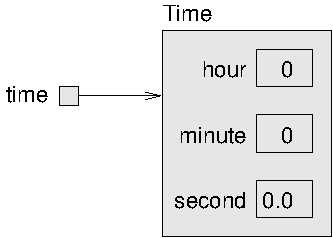
\includegraphics{figs/time.pdf}


After declaring the instance variables, the next step is
to define a constructor for the new class.

\section{Constructors}
\index{constructor}
\index{method!constructor}
\index{static}

Constructors initialize instance
variables.  The syntax for constructors is similar to that
of other methods, with three exceptions:

\begin{itemize}

\item The name of the constructor is the same as the name of
the class.

\item Constructors have no return type and no return value.

\item The keyword {\tt static} is omitted.

\end{itemize}

Here is an example for the {\tt Time} class:

\begin{code}
    public Time() {
        this.hour = 0;
        this.minute = 0;
        this.second = 0.0;
    }
\end{code}

Where you would expect to see a return type,
between {\tt public} and {\tt Time}, there is nothing.  That's
how we (and the compiler) can tell that this is a constructor.

This constructor does not take any arguments.  Each line of the
constructor initializes an instance variable to a default
value (in this case, midnight).  The name {\tt this} is a special
keyword that refers to the object we are creating.  You can use
{\tt this} the same way you use the name of any other object.  For
example, you can read and write the instance variables of {\tt this},
and you can pass {\tt this} as an argument to other methods.

\index{this}

But you do not declare {\tt this} and you can't make an
assignment to it.  {\tt this} is created by the system; all you
have to do is initialize its instance variables.

A common error when writing constructors is to put a {\tt return}
statement at the end.  Resist the temptation.


\section{More constructors}
\index{overloading}

Constructors can be overloaded, just like other methods,
which means that you can provide multiple constructors
with different parameters.  Java knows which constructor
to invoke by matching the arguments of {\tt new}
with the parameters of the constructors.

It is common to have one constructor that takes no
arguments (shown above), and one constructor that takes
a parameter list identical to the list of instance
variables.  For example:

\begin{code}
    public Time(int hour, int minute, double second) {
        this.hour = hour;
        this.minute = minute;
        this.second = second;
    }
\end{code}

The names and types of the parameters are the same as
the names and types of the instance variables.  All the
constructor does is copy the information from the parameters
to the instance variables.

If you look at the documentation for {\tt Point}s
and {\tt Rectangle}s, you will see that both classes provide
constructors like this.  Overloading constructors provides the
flexibility to create an object first and then fill in the
blanks, or to collect all the information before creating
the object.

This might not seem very interesting, and in fact it
is not.  Writing constructors is a boring, mechanical process.
Once you have written two, you will find that you can write them
quickly just by looking at the list of instance
variables.


\section{Creating a new object}
\index{new}
\index{statement!new}

Although constructors look like methods, you never invoke them
directly.  Instead, when you invoke {\tt new}, the system
allocates space for the new object and then
invokes your constructor.

The following program demonstrates two ways to create and
initialize {\tt Time} objects:

\begin{code}
class Time {
    int hour, minute;
    double second;

    public Time() {
        this.hour = 0;
        this.minute = 0;
        this.second = 0.0;
    }

    public Time(int hour, int minute, double second) {
        this.hour = hour;
        this.minute = minute;
        this.second = second;
    }

    public static void main(String[] args) {

        // one way to create and initialize a Time object
        Time t1 = new Time();
        t1.hour = 11;
        t1.minute = 8;
        t1.second = 3.14159;
        System.out.println(t1);

        // another way to do the same thing
        Time t2 = new Time(11, 8, 3.14159);
        System.out.println(t2);
    }
}
\end{code}

In {\tt main}, the first time we invoke {\tt new},
we provide no arguments, so Java invokes the first constructor.
The next few lines assign values to the instance
variables.

The second time we invoke {\tt new}, we provide
arguments that match the parameters of the second constructor.
This way of initializing the instance variables is more concise
and slightly more efficient, but it can be harder to read, since
it is not as clear which values are assigned to which instance
variables.


\section{Printing objects}
\label{printobject}
\index{print}
\index{statement!print}
\index{object!printing}

The output of this program is:

\begin{stdout}
Time@80cc7c0
Time@80cc807
\end{stdout}

When Java prints the value of a user-defined object type, it prints
the name of the type and a special hexadecimal (base 16) code that is
unique for each object.  This code is not meaningful in itself; in
fact, it can vary from machine to machine and even from run to run.
But it can be useful for debugging, in case you want to keep track of
individual objects.

To print objects in a way that is more meaningful to users
(as opposed to programmers), you can write a method
called something like {\tt printTime}:

\begin{code}
    public static void printTime(Time t) {
        System.out.println(t.hour + ":" + t.minute + ":" + t.second);
    }
\end{code}

Compare this method to the version of {\tt printTime} in
Section~\ref{time}.

The output of this method, if we pass either {\tt t1} or {\tt t2} as
an argument, is {\tt 11:8:3.14159}.  Although this is recognizable
as a time, it is not quite in the standard format.  For example, if
the number of minutes or seconds is less than 10, we expect a leading
{\tt 0} as a place-keeper.  Also, we might want to drop the decimal
part of the seconds.  In other words, we want something like
{\tt 11:08:03}.

In most languages, there are simple ways to control the output format
for numbers.  In Java there are no simple ways.

Java provides powerful tools for printing formatted things
like times and dates, and also for interpreting formatted input.
Unfortunately, these tools are not very easy to use, so I am going to
leave them out of this book.  If you want, you can take a look
at the documentation for the {\tt Date} class in the {\tt
java.util} package.
\index{Date}
\index{class!Date}


\section{Operations on objects}
\label{objectops}
\index{object}
\index{operator!object}

In the next few
sections, I demonstrate three kinds of methods that
operate on objects:

\begin{description}

\item[pure function:]  Takes objects as
arguments but does not modify them.  The return value is
either a primitive or a new object created inside the method.

\item[modifier:]  Takes objects as arguments and modifies some
or all of them.  Often returns void. \index{void}

\item[fill-in method:]  One of the arguments is an ``empty''
object that gets filled in by the method.  Technically, this is
a type of modifier.

\end{description}

Often it is possible to write a given method as a pure function, a modifier,
or a fill-in method.  I will discuss the pros and cons of each.


\section{Pure functions}
\index{pure function}
\index{function}
\index{method!pure function}

A method is considered a pure function if the result depends only on
the arguments, and it has no side effects like modifying an argument
or printing something.  The only result of invoking a pure function is
the return value.

One example is {\tt isAfter}, which compares two {\tt Time}s and
returns a {\tt boolean} that indicates whether the first operand
comes after the second:

\begin{code}
    public static boolean isAfter(Time time1, Time time2) {
        if (time1.hour > time2.hour) return true;
        if (time1.hour < time2.hour) return false;

        if (time1.minute > time2.minute) return true;
        if (time1.minute < time2.minute) return false;

        if (time1.second > time2.second) return true;
        return false;
    }
\end{code}

What is the result of this method if the two times are equal?  Does
that seem like the appropriate result for this method?  If you were
writing the documentation for this method, would you mention that case
specifically?

A second example is {\tt addTime}, which calculates the sum of two
times.  For example, if it is {\tt 9:14:30}, and your breadmaker takes
3 hours and 35 minutes, you could use {\tt addTime} to figure out when
the bread will be done.

Here is a rough draft of this method that is not quite right:

\begin{code}
    public static Time addTime(Time t1, Time t2) {
        Time sum = new Time();
        sum.hour = t1.hour + t2.hour;
        sum.minute = t1.minute + t2.minute;
        sum.second = t1.second + t2.second;
        return sum;
    }
\end{code}

Although this method returns a {\tt Time} object, it is not
a constructor.  You should go back and compare the syntax of
a method like this with the syntax of a constructor, because
it is easy to get confused.

Here is an example of how to use this method.  If {\tt currentTime}
contains the current time and {\tt breadTime} contains the amount
of time it takes for your breadmaker to make bread, then you
could use {\tt addTime} to figure out when the bread will be
done.

\begin{code}
    Time currentTime = new Time(9, 14, 30.0);
    Time breadTime = new Time(3, 35, 0.0);
    Time doneTime = addTime(currentTime, breadTime);
    printTime(doneTime);
\end{code}

The output of this program is {\tt 12:49:30.0}, which is
correct.  On the other hand, there are cases where the result
is not correct.  Can you think of one?

The problem is that this method does not deal with cases
where the number of seconds or minutes adds up to more than
60.  In that case, we have to ``carry'' the extra seconds
into the minutes column, or extra minutes into the hours
column.

Here's a corrected version of the method.

\begin{code}
    public static Time addTime(Time t1, Time t2) {
        Time sum = new Time();
        sum.hour = t1.hour + t2.hour;
        sum.minute = t1.minute + t2.minute;
        sum.second = t1.second + t2.second;

        if (sum.second >= 60.0) {
            sum.second -= 60.0;
            sum.minute += 1;
        }
        if (sum.minute >= 60) {
            sum.minute -= 60;
            sum.hour += 1;
        }
        return sum;
    }
\end{code}

Although it's correct, it's starting to get big.  Later
I suggest a much shorter alternative.

\index{increment}
\index{decrement}
\index{operator!increment}
\index{operator!decrement}

This code demonstrates two operators we have not seen before,
{\tt +=} and {\tt -=}.  These operators provide a concise
way to increment and decrement variables.  They are similar
to {\tt ++} and {\tt --}, except (1) they work on {\tt double}s
as well as {\tt int}s, and (2) the amount of the increment
does not have to be 1.  The statement {\tt sum.second -= 60.0;}
is equivalent to {\tt sum.second = sum.second - 60;}


\section{Modifiers}
\index{modifier}
\index{method!modifier}

As an example of a modifier, consider {\tt increment},
which adds a given number of seconds to a {\tt Time} object.
Again, a rough draft of this method looks like:

\begin{code}
    public static void increment(Time time, double secs) {
        time.second += secs;

        if (time.second >= 60.0) {
            time.second -= 60.0;
            time.minute += 1;
        }
        if (time.minute >= 60) {
            time.minute -= 60;
            time.hour += 1;
        }
    }
\end{code}

The first line performs the basic operation; the remainder
deals with the same cases we saw before.

Is this method correct?  What happens if the argument {\tt secs}
is much greater than 60?  In that case, it is not enough to
subtract 60 once; we have to keep doing it until {\tt second}
is below 60.  We can do that by replacing the {\tt if}
statements with {\tt while} statements:

\begin{code}
    public static void increment(Time time, double secs) {
        time.second += secs;

        while (time.second >= 60.0) {
            time.second -= 60.0;
            time.minute += 1;
        }
        while (time.minute >= 60) {
            time.minute -= 60;
            time.hour += 1;
        }
    }
\end{code}

This solution is correct, but not very efficient.
Can you think of a solution that does not require iteration?


\section{Fill-in methods}
\index{fill-in method}
\index{method!fill-in}

Instead of creating a new object every time {\tt addTime} is
invoked, we could require the caller to provide an
object where {\tt addTime} stores the result.  Compare
this to the previous version:

\begin{code}
    public static void addTimeFill(Time t1, Time t2, Time sum) {
        sum.hour = t1.hour + t2.hour;
        sum.minute = t1.minute + t2.minute;
        sum.second = t1.second + t2.second;

        if (sum.second >= 60.0) {
            sum.second -= 60.0;
            sum.minute += 1;
        }
        if (sum.minute >= 60) {
            sum.minute -= 60;
            sum.hour += 1;
        }
    }
\end{code}

The result is stored in {\tt sum}, so the return type is {\tt void}.

Modifiers and fill-in methods are efficient because they
don't have to create new objects.  But they make it more
difficult to isolate parts of a program; in large projects they can
cause errors that are hard to find.

Pure functions help manage the complexity of large projects,
in part by making certain kinds of errors impossible.  Also, they
lend themselves to certain kinds of composition and nesting.
And because the result of a pure function depends only on the parameters,
it is possible to speed them up by storing previously-computed
results.
\index{pure function}

I recommend that you write pure functions whenever
it is reasonable, and resort to modifiers only if there
is a compelling advantage.


\section{Incremental development and planning}
\index{incremental development}
\index{prototyping}
\index{program development!incremental}
\index{program development!planning}

In this chapter I demonstrated a program development process called
{\bf rapid prototyping}\footnote{What I am calling rapid prototyping
  is similar to test-driven development (TDD); the difference is that
  TDD is usually based on automated testing.  See
  \url{http://en.wikipedia.org/wiki/Test-driven_development}.}.  For
each method, I wrote a rough draft that performed the
basic calculation, then tested it on a few cases, correcting flaws
as I found them.

This approach can be effective, but it can lead to code
that is unnecessarily complicated---since it deals with many
special cases---and unreliable---since it is hard to convince
yourself that you have found {\em all} the errors.

An alternative is to look for insight
into the problem that can make the programming easier.  In
this case the insight is that a {\tt Time} is really a three-digit
number in base 60!  The {\tt second} is the ``ones column,''
the {\tt minute} is the ``60's column'', and the {\tt hour}
is the ``3600's column.''

When we wrote {\tt addTime} and {\tt increment}, we were effectively
doing addition in base 60, which is why we had to ``carry'' from one
column to the next.

\index{arithmetic!floating-point}

Another approach to the whole problem is to convert
{\tt Time}s into {\tt double}s and take advantage of the fact that
the computer already knows how to do arithmetic with {\tt double}s.
Here is a method that converts a {\tt Time} into a {\tt double}:

\begin{code}
        public static double convertToSeconds(Time t) {
        int minutes = t.hour * 60 + t.minute;
        double seconds = minutes * 60 + t.second;
        return seconds;
    }
\end{code}

Now all we need is a way to convert from a {\tt double}
to a {\tt Time} object.  We could write a method to
do it, but it might make more sense to write it as a third
constructor:

\begin{code}
    public Time(double secs) {
        this.hour =(int)(secs / 3600.0);
        secs -= this.hour * 3600.0;
        this.minute =(int)(secs / 60.0);
        secs -= this.minute * 60;
        this.second = secs;
    }
\end{code}

This constructor is a little different from the others;
it involves some calculation along with assignments to the
instance variables.

You might have to think to convince yourself that the technique
I am using to convert from one base to another is correct.  But once
you're convinced, we can use these methods to rewrite {\tt addTime}:

\begin{code}
    public static Time addTime(Time t1, Time t2) {
        double seconds = convertToSeconds(t1) + convertToSeconds(t2);
        return new Time(seconds);
    }
\end{code}

This is shorter than the original version, and it is much easier
to demonstrate that it is correct (assuming, as usual, that the
methods it invokes are correct).  As an exercise, rewrite {\tt
increment} the same way.


\section{Generalization}
\index{generalization}

In some ways converting from base 60 to base 10 and back is
harder than just dealing with times.  Base conversion is more
abstract; our intuition for dealing with times is better.

But if we have the insight to treat times as base 60 numbers,
and make the investment of writing the conversion methods
({\tt convertToSeconds} and the third constructor), we get
a program that is shorter, easier to read and debug, and more
reliable.

It is also easier to add features later.  Imagine
subtracting two {\tt Time}s to find the duration between them.  The
naive approach would be to implement subtraction complete with
``borrowing.''  Using the conversion methods would be much easier.

Ironically, sometimes making a problem harder (more general)
makes it easier (fewer special cases, fewer opportunities for error).


\section{Algorithms}
\label{algorithm}
\index{algorithm}

When you write a general solution for a class of problems, as
opposed to a specific solution to a single problem, you have
written an {\bf algorithm}.  This word is
not easy to define, so I will try a couple of approaches.

First, consider some things that are not algorithms.  When you learned
to multiply single-digit numbers, you probably memorized the
multiplication table.  In effect, you memorized 100 specific
solutions, so that knowledge is not really algorithmic.

But if you were ``lazy,'' you probably learned a few
tricks.  For example, to find the product of $n$ and 9, you can
write $n-1$ as the first digit and $10-n$ as the second digit.  This
trick is a general solution for multiplying any single-digit number by 9.
That's an algorithm!

Similarly, the techniques you learned for addition with carrying,
subtraction with borrowing, and long division are all algorithms.  One
of the characteristics of algorithms is that they do not require any
intelligence to carry out.  They are mechanical processes in which
each step follows from the last according to a simple set of rules.

In my opinion, it is embarrassing that humans spend so much
time in school learning to execute algorithms that,
quite literally, require no intelligence.
%
On the other hand, the process of designing algorithms is
interesting, intellectually challenging, and a central part
of what we call programming.

Some of the things that people do naturally, without difficulty
or conscious thought, are the most difficult to express
algorithmically.  Understanding natural language is a good
example.  We all do it, but so far no one has been able to
explain {\em how} we do it, at least not in the form of an
algorithm.

Soon you will have the opportunity to design
simple algorithms for a variety of problems.


\section{Glossary}

\begin{description}

\item[class:]  Previously, I defined a class as a collection
of related methods.  In this chapter we learned that a class
definition is also a template for a new type of object.

\item[instance:]  A member of a class.  Every object is an
instance of some class.

\item[constructor:]  A special method that initializes the instance
variables of a newly-constructed object.

\item[startup class:]  The class that contains the {\tt main}
method where execution of the program begins.

\item[pure function:]  A method whose result depends only on its
parameters, and that has no side-effects other than returning
a value.

\item[modifier:]  A method that changes one or more of the objects
it receives as parameters, and usually returns {\tt void}.

\item[fill-in method:]  A type of method that takes an ``empty''
object as a parameter and fills in its instance variables instead
of generating a return value.

\item[algorithm:]  A set of instructions for solving a class of
problems by a mechanical process.

\index{class}
\index{instance}
\index{constructor}
\index{startup class}
\index{pure function}
\index{modifier}
\index{algorithm}

\end{description}


\section{Exercises}

\begin{exercise}
In the board game Scrabble\footnote{Scrabble is a registered trademark
owned in the U.S.A and Canada by Hasbro Inc., and in the rest of the world
by J.W. Spear \& Sons Limited of Maidenhead, Berkshire, England, a subsidiary
of Mattel Inc.}, each tile contains a letter, which is used to spell
words, and a score, which is used to determine the value of words.

\begin{enumerate}

\item Write a definition for a class named {\tt Tile}
that represents Scrabble tiles.  The instance variables should
be a character named {\tt letter} and an integer named {\tt value}.

\item Write a constructor that takes parameters named {\tt letter}
and {\tt value} and initializes the instance variables.

\item Write a method named {\tt printTile} that takes a {\tt Tile}
object as a parameter and prints the instance variables in
a reader-friendly format.

\item Write a method named {\tt testTile} that creates a
Tile object with the letter {\tt Z} and the value 10, and
then uses {\tt printTile} to print the state of the object.

\end{enumerate}

The point of this exercise is to practice the mechanical part
of creating a new class definition and code that tests it.
\end{exercise}


\begin{exercise}
Write a class definition for {\tt Date}, an object type that
contains three integers, {\tt year}, {\tt month} and {\tt day}.
This class should provide two constructors.  The first should
take no parameters.  The second should take parameters named
{\tt year}, {\tt month} and {\tt day}, and use them to initialize
the instance variables.

Write a {\tt main} method that creates a new {\tt Date} object
named {\tt birthday}.  The new object should contain your birthdate.
You can use either constructor.
\end{exercise}


\begin{exercise}
\label{ex.rational}

A rational number is a number that can be represented as the ratio of
two integers.  For example, $2/3$ is a rational number, and you can
think of 7 as a rational number with an implicit 1 in the denominator.
For this assignment, you are going to write a class definition for
rational numbers.

\begin{enumerate}

\item Create a new program called {\tt Rational.java} that defines a
class named {\tt Rational}.  A {\tt Rational} object should have two
integer instance variables to store the numerator and denominator.

\item Write a constructor that takes no arguments and that sets the
numerator to 0 and denominator to 1.

\item Write a method called {\tt printRational} that takes
a Rational object as an argument and prints it in some
reasonable format.

\item Write a {\tt main} method that creates a new object with
type Rational, sets its instance variables to some values, and prints
the object.

\item At this stage, you have a minimal testable
program.  Test it and, if necessary, debug it.

\item Write a second constructor for your class that takes two
arguments and that uses them to initalize the instance
variables.

\item Write a method called {\tt negate} that reverses the sign of
a rational number.  This method should be a modifier, so it should
return {\tt void}.  Add lines to {\tt main} to test the new method.

\item Write a method called {\tt invert} that inverts the number by
  swapping the numerator and denominator.  Add lines to {\tt main} to
  test the new method.

\item Write a method called {\tt toDouble} that converts the rational
number to a double (floating-point number) and returns the result.
This method is a pure function; it does not modify the object.
As always, test the new method.

\item Write a modifier named {\tt reduce} that reduces a rational
  number to its lowest terms by finding the greatest common divisor
  (GCD) of the numerator and denominator and dividing through.
  This method should be a pure function; it should
  not modify the instance variables of the object on which it is
  invoked.  To find the GCD, see Exercise~\ref{gcd}).

\item Write a method called {\tt add} that takes two Rational
numbers as arguments and returns a new Rational object.  The return
object should contain the sum of the arguments.

There are several ways to add fractions.  You can use any one you
want, but you should make sure that the result of the operation is
reduced so that the numerator and denominator have no common divisor
(other than 1).
\end{enumerate}

The purpose of this exercise is to write a class definition that
includes a variety of methods, including constructors, modifiers and
pure functions.
\end{exercise}





%\chapter{Arrays}
\label{chap10}
\label{arrays}
\index{array}
\index{type!array}

An {\bf array} is a set of values where each value is identified by an
index.  You can make an array of {\tt int}s, {\tt double}s, or any
other type, but all the values in an array have to have the same type.

Syntactically, array types look like other Java types except they are
followed by {\tt []}.  For example, {\tt int[]} is the type ``array of
integers'' and {\tt double[]} is the type ``array of doubles.''

You can declare variables with these types in the usual ways:

\begin{code}
    int[] count;
    double[] values;
\end{code}

Until you initialize these variables, they are set to {\tt null}.
To create the array itself, use {\tt new}.

\begin{code}
    count = new int[4];
    values = new double[size];
\end{code}

The first assignment makes {\tt count} refer to an array of 4
integers; the second makes {\tt values} refer to an array of {\tt
double}s.  The number of elements in {\tt values} depends on {\tt
size}.  You can use any integer expression as an array
size.

\index{null}
\index{state diagram}

The following figure shows how arrays are represented in state
diagrams:


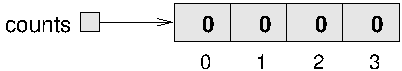
\includegraphics{figs/array.pdf}


The large numbers inside the boxes are the {\bf elements} of
the array.  The small numbers outside the boxes are the
indices used to identify each box.  When you allocate an
array of {\tt int}s, the elements are initialized to zero.


\section{Accessing elements}
\index{element}
\index{array!element}

To store values in the array, use the
{\tt []} operator.  For example {\tt count[0]} refers to the
``zeroeth'' element of the array, and {\tt count[1]} refers to the
``oneth'' element.  You can use the {\tt []} operator anywhere in an
expression:

\begin{code}
    count[0] = 7;
    count[1] = count[0] * 2;
    count[2]++;
    count[3] -= 60;
\end{code}

These are all legal assignment statements.  Here is the
result of this code fragment:


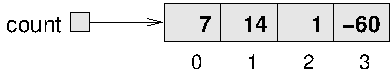
\includegraphics{figs/array2.pdf}


The elements of the array
are numbered from 0 to 3, which means that there is no element with
the index 4.  This should sound familiar, since we saw the same thing
with {\tt String} indices.  Nevertheless, it is a common error to go
beyond the bounds of an array, which throws an {\tt
ArrayOutOfBoundsException}.
\index{exception!ArrayOutOfBounds}
\index{run-time error}
\index{index}

You can use any expression as an index, as long as it has type {\tt
int}.  One of the most common ways to index an array is with a loop
variable.  For example:
\index{expression}

\begin{code}
    int i = 0;
    while (i < 4) {
        System.out.println(count[i]);
        i++;
    }
\end{code}

This is a standard {\tt while} loop that counts from 0
up to 4, and when the loop variable {\tt i} is 4, the
condition fails and the loop terminates.  Thus, the body
of the loop is only executed when {\tt i} is 0, 1, 2 and 3.

\index{loop}
\index{loop variable}
\index{variable!loop}

Each time through the loop we use {\tt i} as an index into
the array, printing the {\tt i}th element.  This type of
array traversal is very common.


\section{Copying arrays}
\index{array!copying}

When you copy an array variable, remember that you are
copying a reference to the array.  For example:

\begin{code}
    double[] a = new double[4];
    double[] b = a;
\end{code}

This code creates one array of three {\tt double}s, and
sets two different variables to refer to it.
This situation is a form of aliasing.


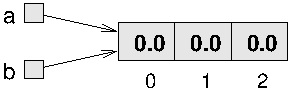
\includegraphics{figs/array3.pdf}


Any changes in either array
will be reflected in the other.  This is not usually the
behavior you want; more often you want to
allocate a new array and copy elements from
one to the other.

\begin{code}
    double[] b = new double[4];

    int i = 0;
    while (i < 4) {
      b[i] = a[i];
      i++;
    }
\end{code}


\section{Arrays and objects}
\index{object!compared to array}
\index{array!compared to object}

In many ways, arrays behave like objects:

\begin{itemize}

\item When you declare an array variable, you get a reference
to an array.

\item You have to use {\tt new} to create the array itself.

\item When you pass an array as an argument, you pass a reference,
which means that the invoked method can change the contents
of the array.

\end{itemize}

Some of the objects we looked at, like {\tt Rectangles}, are
similar to arrays in the sense that they are collections of
values.  This raises the question, ``How is an array of 4 integers
different from a Rectangle object?''
\index{collection}

If you go back to the definition of ``array'' at the beginning
of the chapter, you see one difference: the
elements of an array are identified by indices, and the
elements of an object have names.

Another difference is that the
elements of an array have to be the same type.  Objects can
have instance variables with different types.


\section{{\tt for} loops}
\label{for}

The loops we have written have a number of elements
in common.  All of them start by initializing a variable;
they have a test, or condition, that depends on that variable;
and inside the loop they do something to that variable,
like increment it.

\index{loop!for}
\index{for}
\index{statement!for}

This type of loop is so common that there is another
loop statement, called {\tt for}, that expresses it more
concisely.  The general syntax looks like this:

\begin{code}
    for (INITIALIZER; CONDITION; INCREMENTOR) {
        BODY
    }
\end{code}

This statement is equivalent to

\begin{code}
    INITIALIZER;
    while (CONDITION) {
        BODY
        INCREMENTOR
    }
\end{code}

except that it is more concise and, since it puts all the
loop-related statements in one place, it is easier to read.
For example:

\begin{code}
    for (int i = 0; i < 4; i++) {
        System.out.println(count[i]);
    }
\end{code}

is equivalent to

\begin{code}
    int i = 0;
    while (i < 4) {
        System.out.println(count[i]);
        i++;
    }
\end{code}


\section{Array length}
\index{length!array}
\index{array!length}

All arrays have one named instance variable: {\tt length}.
Not surprisingly, it contains the length of the array (number
of elements).  It is a good idea to use this value as the upper
bound of a loop, rather than a constant value.  That way, if
the size of the array changes, you won't have to go through the
program changing all the loops; they will work correctly for any
size array.

\begin{code}
    for (int i = 0; i < a.length; i++) {
        b[i] = a[i];
    }
\end{code}

The last time the body of the loop gets executed, {\tt i}
is {\tt a.length - 1}, which is the index of the last element.  When
{\tt i} is equal to {\tt a.length}, the condition fails and the body
is not executed, which is a good thing, since it would throw an
exception.  This code assumes that the array {\tt b} contains at least
as many elements as {\tt a}.


\section{Random numbers}
\label{random}
\label{pseudorandom}
\index{random number}
\index{deterministic}
\index{nondeterministic}

Most computer programs do the same thing every time they are executed,
so they are said to be {\bf deterministic}.  Usually, determinism is a
good thing, since we expect the same calculation to yield the same
result.  But for some applications we want the
computer to be unpredictable.  Games are an obvious example, but
there are more.

Making a program truly {\bf nondeterministic} turns out to be not so
easy, but there are ways to make it at least seem nondeterministic.
One of them is to generate random numbers and use them to determine
the outcome of the program.  Java provides a method that generates
{\bf pseudorandom} numbers, which may not be truly random, but for our
purposes, they will do.

Check out the documentation of the {\tt random} method in the {\tt
Math} class.  The return value is a {\tt double} between 0.0 and 1.0.
To be precise, it is greater than or equal to 0.0 and strictly less
than 1.0.  Each time you invoke {\tt random} you get the next
number in a pseudorandom sequence.
To see a sample, run this loop:

\begin{code}
    for (int i = 0; i < 10; i++) {
        double x = Math.random();
        System.out.println(x);
    }
\end{code}

To generate a random {\tt double} between 0.0 and an upper bound like
{\tt high}, you can multiply {\tt x} by {\tt high}.


\section{Array of random numbers}
\label{randarray}

How would you generate a random integer between {\tt low} and {\tt high}?
If your implementation of {\tt randomInt} is correct, then
every value in the range from {\tt low} to {\tt high-1} should
have the same probability.  If you generate a long series
of numbers, every value should appear, at least approximately,
the same number of times.

One way to test your method is to
generate a large number of random values,
store them in an array, and count the number of times each
value occurs.

The following method takes a single argument, the size of
the array.  It allocates a new array of integers, fills
it with random values, and returns a reference to the new
array.

\begin{code}
  public static int[] randomArray(int n) {
      int[] a = new int[n];
      for (int i = 0; i<a.length; i++) {
          a[i] = randomInt(0, 100);
      }
      return a;
  }
\end{code}

The return type is {\tt int[]}, which means that
this method returns an array of integers.
To test this method, it is convenient to have a method that
prints the contents of an array.

\begin{code}
  public static void printArray(int[] a) {
      for (int i = 0; i<a.length; i++) {
          System.out.println(a[i]);
      }
  }
\end{code}

The following code generates an array and prints it:

\begin{code}
    int numValues = 8;
    int[] array = randomArray(numValues);
    printArray(array);
\end{code}

On my machine the output is

\begin{stdout}
27
6
54
62
54
2
44
81
\end{stdout}

which is pretty random-looking.  Your results may differ.

If these were exam scores (and they would be pretty bad exam
scores) the teacher might present the results to the class
in the form of a {\bf histogram}, which is a set of counters
that keeps track of the number of times each value appears.

\index{histogram}

For exam scores, we might have ten counters to keep track of
how many students scored in the 90s, the 80s, etc.  The next
few sections develop code to generate a histogram.


\section{Counting}
\index{traverse!array}
\index{array!traverse}
\index{looping and counting}
\index{counter}

A good approach to problems like this is to think of simple methods
that are easy to write, then combine them into a solution.
This process is called {\bf bottom-up development}.
See \url{http://en.wikipedia.org/wiki/Top-down_and_bottom-up_design}.
\index{program development}

It is not always obvious where to start,
but a good approach is to look for subproblems that fit a pattern you
have seen before.

In Section~\ref{loopcount} we saw a loop that traversed a
string and counted the number of times a given letter appeared.  You
can think of this program as an example of a pattern called ``traverse
and count.''  The elements of this pattern are:

\begin{itemize}

\item A set or container that can be traversed, like an array
or a string.

\item A test that you can apply to each element in the container.

\item A counter that keeps track of how many elements pass
the test.

\end{itemize}

In this case, the container is an array of integers.  The
test is whether or not a given score falls in a given range of
values.

Here is a method called {\tt inRange} that counts the number of
elements in an array that fall in a given range.  The parameters are
the array and two integers that specify the lower and upper bounds of
the range.

\begin{code}
public static int inRange(int[] a, int low, int high) {
    int count = 0;
    for (int i = 0; i < a.length; i++) {
        if (a[i] >= low && a[i] < high) count++;
    }
    return count;
}
\end{code}

I wasn't specific about whether something equal
to {\tt low} or {\tt high} falls in the range, but you can
see from the code that {\tt low} is in and {\tt high} is out.
That keeps us from counting any elements twice.

Now we can count the number of scores in the ranges we are
interested in:

\begin{code}
int[] scores = randomArray(30);
int a = inRange(scores, 90, 100);
int b = inRange(scores, 80, 90);
int c = inRange(scores, 70, 80);
int d = inRange(scores, 60, 70);
int f = inRange(scores, 0, 60);
\end{code}


\section{The histogram}
\index{range}
\index{histogram}

This code is repetitious, but it is acceptable as
long as the number of ranges is small.  But imagine that
we want to keep track of the number of times each score appears,
all 100 possible values.  Would you want to write this?

\begin{code}
int count0 = inRange(scores, 0, 1);
int count1 = inRange(scores, 1, 2);
int count2 = inRange(scores, 2, 3);
...
int count3 = inRange(scores, 99, 100);
\end{code}

I don't think so.  What we really want is a way to store 100 integers,
preferably so we can use an index to access each one.  Hint: array.

The counting pattern is the same whether we use a single counter or an
array of counters.  In this case, we initialize the array outside the
loop; then, inside the loop, we invoke {\tt inRange} and store the
result:

\begin{code}
    int[] counts = new int[100];

    for (int i = 0; i < counts.length; i++) {
        counts[i] = inRange(scores, i, i+1);
    }
\end{code}

The only tricky thing here is that we are using the loop variable
in two roles: as in index into the array, and as the parameter to
{\tt inRange}.


\section{A single-pass solution}
\label{singlepass}

This code works, but it is not as efficient as it could
be.  Every time it invokes {\tt inRange}, it traverses the
entire array.  As the number of ranges increases, that gets
to be a lot of traversals.

It would be better to make a single pass through the array,
and for each value, compute which range it falls in.  Then
we could increment the appropriate counter.
In this example, that computation is trivial, because we
can use the value itself as an index into the array of counters.

Here is code that traverses an array of scores once and generates
a histogram.

\begin{code}
    int[] counts = new int[100];

    for (int i = 0; i < scores.length; i++) {
        int index = scores[i];
        counts[index]++;
    }
\end{code}


\section{Glossary}

\begin{description}

\item[array:]  A collection of values, where all the
values have the same type, and each value is identified by
an index.

\item[element:]  One of the values in an array.  The {\tt []}
operator selects elements.

\item[index:]  An integer variable or value used to indicate
an element of an array.

\item[deterministic:]  A program that does the same thing every
time it is invoked.

\item[pseudorandom:]  A sequence of numbers that appear to be
random, but which are actually the product of a deterministic
computation.

\item[histogram:]  An array of integers where each integer
counts the number of values that fall into a certain range.

\index{array}
\index{element}
\index{index}
\index{deterministic}
\index{pseudorandom}

\end{description}


\section{Exercises}

\begin{exercise}
Write a method called {\tt cloneArray} that takes an
array of integers as a parameter, creates a new array that is the same
size, copies the elements from the first array into the new one, and
then returns a reference to the new array.
\end{exercise}


\begin{exercise}
Write a method called {\tt randomDouble} that takes two doubles,
{\tt low} and {\tt high}, and that returns a random double $x$
so that $low \le x < high$.
\end{exercise}


\begin{exercise}
\label{ex.randint}
Write a method called {\tt randomInt} that takes two arguments,
{\tt low} and {\tt high}, and that returns a random integer between
{\tt low} and {\tt high}, not including {\tt high}.
\end{exercise}


\begin{exercise}
Encapsulate the code in Section~\ref{singlepass} in a method called
{\tt makeHist} that takes an array of scores and returns a histogram
of the values in the array.
\end{exercise}


\begin{exercise}
Write a method named {\tt areFactors} that takes
an integer {\tt n} and an array of integers, and that returns
{\tt true} if the numbers in the array are all factors of {\tt n}
(which is to say that {\tt n} is divisible by all of them).
HINT: See Exercise~\ref{ex.isdiv}.
\end{exercise}


\begin{exercise}
Write a method that takes an array of integers and an integer named
{\tt target} as arguments, and that returns the first index where
{\tt target} appears in the array, if it does, and -1 otherwise.
\end{exercise}


\begin{exercise}
Some programmers disagree with the general rule that variables
and methods should be given meaningful names.  Instead, they
think variables and methods should be named after fruit.

For each of the following methods, write one sentence that
describes abstractly what the method does.  For each variable,
identify the role it plays.

\begin{code}
public static int banana(int[] a) {
    int grape = 0;
    int i = 0;
    while (i < a.length) {
        grape = grape + a[i];
        i++;
    }
    return grape;
}

public static int apple(int[] a, int p) {
    int i = 0;
    int pear = 0;
    while (i < a.length) {
        if (a[i] == p) pear++;
        i++;
    }
    return pear;
}

public static int grapefruit(int[] a, int p) {
    for (int i = 0; i<a.length; i++) {
        if (a[i] == p) return i;
    }
    return -1;
}
\end{code}

The purpose of this exercise is to practice reading code and
recognizing the computation patterns we have seen.
\end{exercise}


\begin{exercise}
\begin{enumerate}

\item What is the output of the following program?

\item Draw a stack diagram that shows the state of the
program just before {\tt mus} returns.

\item Describe in a few words what {\tt mus} does.
\end{enumerate}

\begin{code}
public static int[] make(int n) {
    int[] a = new int[n];

    for (int i = 0; i < n; i++) {
        a[i] = i+1;
    }
    return a;
}

public static void dub(int[] jub) {
    for (int i = 0; i < jub.length; i++) {
        jub[i] *= 2;
    }
}

public static int mus(int[] zoo) {
    int fus = 0;
    for (int i = 0; i < zoo.length; i++) {
        fus = fus + zoo[i];
    }
    return fus;
}

public static void main(String[] args) {
    int[] bob = make(5);
    dub(bob);

    System.out.println(mus(bob));
}
\end{code}
\end{exercise}


\begin{exercise}
Many of the patterns we have seen for traversing arrays can
also be written recursively.  It is not common to do so, but
it is a useful exercise.

\begin{enumerate}

\item Write a method called {\tt maxInRange} that takes an array of
integers and a range of indices ({\tt lowIndex} and {\tt highIndex}),
and that finds the maximum value in the array, considering only the
elements between {\tt lowIndex} and {\tt highIndex}, including both
ends.

This method should be recursive.  If the length of the range is 1,
that is, if {\tt lowIndex == highIndex}, we know immediately that the
sole element in the range must be the maximum.  So that's the base
case.

If there is more than one element in the range, we can break the array
into two pieces, find the maximum in each of the pieces, and then find
the maximum of the maxima.

\item Methods like {\tt maxInRange} can be awkward to use.  To
find the largest element in an array, we have to provide a range
that includes the entire array.

\begin{code}
    double max = maxInRange(array, 0, a.length-1);
\end{code}

Write a method called {\tt max} that takes an array as a parameter
and that uses {\tt maxInRange} to find and return the largest value.
Methods like {\tt max} are sometimes called {\bf wrapper methods}
because they provide a layer of abstraction around an awkward method
and make it easier to use.  The method that actually
performs the computation is called the {\bf helper method}.

\item Write a recursive method named {\tt find} using the
wrapper-helper pattern.  {\tt find} should take an array of
integers and a target integer.  It should return the index
of the first location where the target integer appears in the
array, or -1 if it does not appear.

\end{enumerate}
\end{exercise}

\begin{exercise}
One not-very-efficient way to sort the elements of an array
is to find the largest element and swap it with the first
element, then find the second-largest element and swap it with
the second, and so on.  This method is called a {\bf selection
sort} (see \url{http://en.wikipedia.org/wiki/Selection_sort}).

\begin{enumerate}

\item Write a method called {\tt indexOfMaxInRange} that
takes an array of integers, finds the
largest element in the given range, and returns its {\em index}.
You can modify your recursive version of {\tt maxInRange} or
you can write an iterative version from scratch.

\item Write a method called {\tt swapElement} that takes an
array of integers and two indices, and that swaps the elements
at the given indices.

\item Write a method called {\tt selectionSort} that takes an array of
integers and that uses {\tt indexOfMaxInRange} and {\tt swapElement}
to sort the array from largest to smallest.

\end{enumerate}
\end{exercise}


\begin{exercise}
Write a method called {\tt letterHist} that takes a String as a
parameter and that returns a histogram of the letters in the String.
The zeroeth element of the histogram should contain the number of a's
in the String (upper and lower case); the 25th element should contain
the number of z's.
Your solution should only traverse the String once.
\end{exercise}


\begin{exercise}
A word is said to be a ``doubloon'' if every letter that appears in the
word appears exactly twice.  For example, the following are all the
doubloons I found in my dictionary.

\begin {quote}
Abba, Anna, appall, appearer, appeases, arraigning, beriberi,
bilabial, boob, Caucasus, coco, Dada, deed, Emmett, Hannah,
horseshoer, intestines, Isis, mama, Mimi, murmur, noon, Otto, papa,
peep, reappear, redder, sees, Shanghaiings, Toto
\end{quote}

Write a method called {\tt isDoubloon} that returns {\tt true}
if the given word is a doubloon and {\tt false} otherwise.
\end{exercise}


\begin{exercise}
Two words are anagrams if they contain the same letters (and the
same number of each letter).  For example, ``stop'' is an anagram
of ``pots'' and ``allen downey'' is an anagram of ``well annoyed.''

Write a method that takes two Strings and returns {\tt true} if
the Strings are anagrams of each other.

Optional challenge: read the letters of the Strings only once.
\end{exercise}


\begin{exercise}
In Scrabble each player has a set of tiles with letters on them, and
the object of the game is to use those letters to spell words.  The
scoring system is complicated, but longer words are usually
worth more than shorter words.

Imagine you are given your set of tiles as a String, like {\tt
"quijibo"} and you are given another String to test, like {\tt "jib"}.
Write a method called {\tt canSpell} that takes two Strings and
returns {\tt true} if the set of tiles can be used to spell the word.  You
might have more than one tile with the same letter, but you can only
use each tile once.

Optional challenge: read the letters of the Strings only once.
\end{exercise}


\begin{exercise}
In real Scrabble, there are some blank tiles that can be used
as wild cards; that is, a blank tile can be used to represent
any letter.

Think of an algorithm for {\tt canSpell} that deals with wild
cards.  Don't get bogged down in details of implementation like
how to represent wild cards.  Just describe the algorithm, using
English, pseudocode, or Java.
\end{exercise}




%\chapter{Arrays of Objects}
\label{chap11}


\section{The Road Ahead}
\index{composition}
\index{nested structure}

In the next three chapters we will develop programs to work with
playing cards and decks of cards.  Before we dive in, here is an
outline of the steps:

\begin{enumerate}

\item In this chapter we'll define a {\tt Card} class and write
methods that work with {\tt Cards} and arrays of {\tt Cards}.

\item In Chapter~\ref{chap12} we will create a {\tt Deck} class
and write methods that operate on {\tt Deck}s.

\item In Chapter~\ref{chap13} I will present object-oriented
programming (OOP) and we will transform the {\tt Card} and {\tt Deck}
classes into a more OOP style.

\end{enumerate}

I think that way of proceeding makes the road smoother; the drawback
is that we will see several versions of the same code, which can
be confusing.  If it helps, you can download the code for each
chapter as you go along.  The code for this chapter is here:
\url{http://thinkapjava.com/code/Card1.java}.


\section{{\tt Card} objects}
\label{card}
\index{Card}
\index{class!Card}

If you are not familiar with common playing cards, now would be a good
time to get a deck, or else this chapter might not make much sense.
Or read \url{http://en.wikipedia.org/wiki/Playing_card}.

There are 52 cards in a deck; each belongs to one of four
suits and one of 13 ranks.  The suits are Spades, Hearts, Diamonds and
Clubs (in descending order in Bridge).  The ranks are Ace, 2, 3, 4, 5,
6, 7, 8, 9, 10, Jack, Queen and King.  Depending on what game you are
playing, the Ace may be considered higher than King or lower than 2.

\index{rank}
\index{suit}

If we want to define a new object to represent a playing card, it is
pretty obvious what the instance variables should be: {\tt rank} and
{\tt suit}.  It is not as obvious what type the instance variables
should be.  One possibility is {\tt String}s, containing things like
{\tt "Spade"} for suits and {\tt "Queen"} for ranks.  One problem with
this implementation is that it would not be easy to compare cards to
see which had higher rank or suit.

\index{encode}
\index{encrypt}
\index{map to}

An alternative is to use integers to {\bf encode} the ranks and
suits.  By ``encode'' I do not mean what some people think, which
is to encrypt or translate into a secret code.  What a computer
scientist means by ``encode'' is something like ``define a mapping
between a sequence of numbers and the things I want to represent.''
For example,

\begin{tabular}{l c l}
Spades & $\mapsto$ & 3 \\
Hearts & $\mapsto$ & 2 \\
Diamonds & $\mapsto$ & 1 \\
Clubs & $\mapsto$ & 0
\end{tabular}

The obvious feature of this mapping is that the suits map to
integers in order, so we can compare suits by comparing integers.
The mapping for ranks is fairly obvious; each of the numerical
ranks maps to the corresponding integer, and for face cards:

\begin{tabular}{l c l}
Jack & $\mapsto$ & 11 \\
Queen & $\mapsto$ & 12 \\
King & $\mapsto$ & 13 \\
\end{tabular}

The reason I am using mathematical notation for these mappings is
that they are not part of the program.  They are part of the
program design, but they never appear explicitly in the code.
The class definition for the {\tt Card} type looks like this:

\begin{code}
class Card
{
    int suit, rank;

    public Card() {
        this.suit = 0;  this.rank = 0;
    }

    public Card(int suit, int rank) {
        this.suit = suit;  this.rank = rank;
    }
}
\end{code}

As usual, I provide two constructors: one takes
a parameter for each instance variable; the other
takes no parameters.

\index{constructor}

To create an object that represents the 3 of Clubs, we invoke {\tt new}:

\begin{code}
    Card threeOfClubs = new Card(0, 3);
\end{code}

The first argument, {\tt 0} represents the suit Clubs.


\section{The {\tt printCard} method}
\label{printcard}
\index{print!Card}

When you create a new class, the first step is to declare the
instance variables and write constructors.  The second step is
to write the standard methods that every object should have, including
one that prints the object, and one or two that compare objects.
Let's start with {\tt printCard}.

\index{String!array of}
\index{array!of String}

To print {\tt Card} objects in a way that humans
can read easily, we want to map the integer codes onto words.
A natural way to do that is with an array of {\tt String}s.  You
can create an array of {\tt String}s the same way you create an
array of primitive types:

\begin{code}
    String[] suits = new String[4];
\end{code}

Then we can set the values of the elements of the array.

\begin{code}
    suits[0] = "Clubs";
    suits[1] = "Diamonds";
    suits[2] = "Hearts";
    suits[3] = "Spades";
\end{code}

Creating an array and initializing the elements is such a common
operation that Java provides a special syntax for it:

\begin{code}
    String[] suits = { "Clubs", "Diamonds", "Hearts", "Spades" };
\end{code}

This statement is equivalent to the
separate declaration, allocation, and assignment.  The state
diagram of this array looks like:

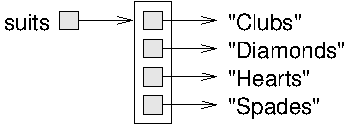
\includegraphics{figs/stringarray.pdf}

\index{state diagram}
\index{reference}
\index{String!reference to}

The elements of the array are {\em references} to the {\tt String}s,
rather than {\tt String}s themselves.

Now we need another array of {\tt String}s to decode the ranks:

\begin{code}
    String[] ranks = { "narf", "Ace", "2", "3", "4", "5", "6",
               "7", "8", "9", "10", "Jack", "Queen", "King" };
\end{code}

The reason for the {\tt "narf"} is to act as a place-keeper for the
zeroeth element of the array, which is never used (or shouldn't be).
The only valid ranks are 1--13.  To avoid this wasted element,
we could have started at 0, but the mapping is more natural if we
encode 2 as 2, and 3 as 3, etc.

Using these arrays, we can select the appropriate {\tt String}s by
using the {\tt suit} and {\tt rank} as indices.  In the method
{\tt printCard},

\begin{code}
public static void printCard(Card c) {
    String[] suits = { "Clubs", "Diamonds", "Hearts", "Spades" };
    String[] ranks = { "narf", "Ace", "2", "3", "4", "5", "6",
               "7", "8", "9", "10", "Jack", "Queen", "King" };

    System.out.println(ranks[c.rank] + " of " + suits[c.suit]);
}
\end{code}

the expression {\tt suits[c.suit]} means ``use the instance variable
{\tt suit} from the object {\tt c} as an index into the array named
{\tt suits}, and select the appropriate string.''  The output of this
code

\begin{code}
    Card card = new Card(1, 11);
    printCard(card);
\end{code}

is {\tt Jack of Diamonds}.


\section{The {\tt sameCard} method}
\label{equivalence}
\index{sameCard}

The word ``same'' is one of those things that occur in natural
language that seem perfectly clear until you give it some thought,
and then you realize there is more to it than you expected.
\index{ambiguity}
\index{natural language}
\index{language!natural}

For example, if I say ``Chris and I have the same car,'' I
mean that his car and mine are the same make and model, but they are
two different cars.  If I say ``Chris and I have the same mother,'' I
mean that his mother and mine are one person.  So the
idea of ``sameness'' is different depending on the context.

When you talk about objects, there is a similar ambiguity.  For
example, if two {\tt Card}s are the same, does that mean they
contain the same data (rank and suit), or they are actually
the same {\tt Card} object?

To see if two references refer to the same object, we use
the {\tt ==} operator.  For example:

\begin{code}
    Card card1 = new Card(1, 11);
    Card card2 = card1;

    if (card1 == card2) {
        System.out.println("card1 and card2 are identical.");
    }
\end{code}

References to
the same object are {\bf identical}.  References
to objects with same data are {\bf equivalent}.
\index{equivalent}
\index{identical}

To check equivalence, it
is common to write a method with a name like {\tt sameCard}.

\begin{code}
    public static boolean sameCard(Card c1, Card c2) {
        return(c1.suit == c2.suit && c1.rank == c2.rank);
    }
\end{code}

Here is an example that creates two objects with the same data,
and uses {\tt sameCard} to see if they are equivalent:

\begin{code}
    Card card1 = new Card(1, 11);
    Card card2 = new Card(1, 11);

    if (sameCard(card1, card2)) {
        System.out.println("card1 and card2 are equivalent.");
    }
\end{code}

If references are identical, they are also equivalent,
but if they are equivalent, they are not necessarily identical.

In this case, {\tt card1} and {\tt card2}
are equivalent but not identical, so
the state diagram looks like this:

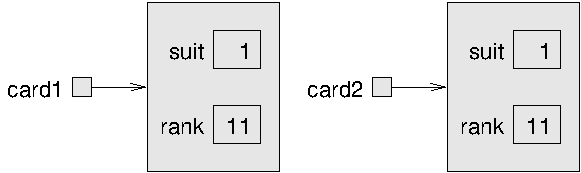
\includegraphics{figs/card.pdf}

What does it look like when
{\tt card1} and {\tt card2} are identical?
\index{aliasing}

In Section~\ref{incomparable} I said that you should not use the
{\tt ==} operator on {\tt String}s because it does not do what you
expect.  Instead of comparing the contents of the {\tt String}
(equivalence), it checks whether the two {\tt String}s are the same
object (identity).


\section{The {\tt compareCard} method}
\label{compare}
\index{compareCard}
\index{operator!conditional}
\index{conditional operator}

For primitive types, the conditional operators
compare values and determine when one is greater or less
than another.  These operators ({\tt <} and {\tt >} and the others)
don't work for object types.  For {\tt String}s Java provides
a {\tt compareTo} method.  For {\tt Card}s we have
to write our own, which we will call {\tt compareCard}.
Later, we will use this method to sort a deck of cards.

\index{ordering}
\index{complete ordering}
\index{partial ordering}

Some sets are completely ordered, which means that you can compare any
two elements and tell which is bigger.  Integers and floating-point
numbers are totally ordered.  Some sets are unordered, which means
that there is no meaningful way to say that one element is bigger than
another.  Fruits are unordered, which is why we cannot compare apples
and oranges.  In Java, the {\tt boolean} type is unordered; we cannot
say that {\tt true} is greater than {\tt false}.

The set of playing cards is partially ordered, which means that
sometimes we can compare cards and sometimes not.  For example, I know
that the 3 of Clubs is higher than the 2 of Clubs, and the 3 of
Diamonds is higher than the 3 of Clubs.  But which is better, the 3 of
Clubs or the 2 of Diamonds?  One has a higher rank, but the other has
a higher suit.
\index{comparable}

To make cards comparable, we have to decide which is more
important, rank or suit.  The choice is
arbitrary, but when you buy a new deck of cards, it comes sorted
with all the Clubs together, followed by all the Diamonds, and so on.
So let's say that suit is more important.

With that decided, we can write {\tt compareCard}.  It
takes two {\tt Card}s as parameters and returns 1 if
the first card wins, -1 if the second card wins, and 0 if
they are equivalent.

First we compare suits:

\begin{code}
    if (c1.suit > c2.suit) return 1;
    if (c1.suit < c2.suit) return -1;
\end{code}

If neither statement is true, the suits must be equal,
and we have to compare ranks:

\begin{code}
    if (c1.rank > c2.rank) return 1;
    if (c1.rank < c2.rank) return -1;
\end{code}

If neither of these is true, the ranks must be equal,
so we return {\tt 0}.


\section{Arrays of cards}
\label{cardarray}
\index{array!of object}
\index{object!array of}
\index{deck}

By now we have seen several examples of composition (the ability to
combine language features in a variety of arrangements).  One of the
first examples we saw was using a method invocation as part of an
expression.  Another example is the nested structure of statements:
you can put an {\tt if} statement within a {\tt while} loop, or within
another {\tt if} statement, etc.
\index{composition}

Having seen this pattern, and having learned about arrays and objects,
you should not be surprised to learn that you can make arrays of
objects.  And you can define objects with arrays as
instance variables; you can make arrays that contain arrays; you can
define objects that contain objects, and so on.
In the next two chapters we will see examples of these
combinations using {\tt Card} objects.

This example creates an array of 52 cards:

\begin{code}
    Card[] cards = new Card[52];
\end{code}

Here is the state diagram for this object:

\index{state diagram}

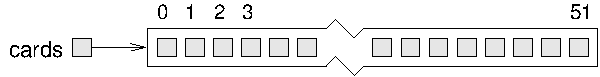
\includegraphics{figs/cardarray.pdf}

The array contains
{\em references} to objects; it does not contain the
{\tt Card} objects themselves.  The elements are
initialized to {\tt null}.  You can access the elements of
the array in the usual way:

\begin{code}
    if (cards[0] == null) {
        System.out.println("No cards yet!");
    }
\end{code}

But if you try to access the instance variables of the
non-existent {\tt Card}s, you get a {\tt NullPointerException}.
\index{exception!NullPointer}
\index{run-time error}
\index{null}

\begin{code}
    cards[0].rank;             // NullPointerException
\end{code}

But that is the correct syntax for accessing the {\tt
rank} of the ``zeroeth'' card in the deck.  This is another example of
  composition, combining the syntax for accessing an element
  of an array and an instance variable of an object.

\index{composition}
\index{loop!nested}

The easiest way to populate the deck with {\tt Card} objects
is to write nested for loops (i.e., one loop inside the body of another):

\begin{code}
    int index = 0;
    for (int suit = 0; suit <= 3; suit++) {
        for (int rank = 1; rank <= 13; rank++) {
            cards[index] = new Card(suit, rank);
            index++;
        }
    }
\end{code}

The outer loop enumerates the suits from 0 to 3.  For
each suit, the inner loop enumerates the ranks from 1
to 13.  Since the outer loop runs 4 times, and
the inner loop runs 13 times,
the body is executed is 52 times.

\index{index}

I used {\tt index} to keep track of where in the
deck the next card should go.  The following state diagram
shows what the deck looks like after the first two cards
have been allocated:

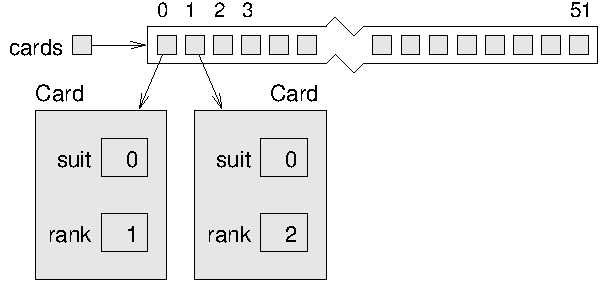
\includegraphics{figs/cardarray2.pdf}


\section{The {\tt printDeck} method}
\label{printdeck}
\index{printDeck}
\index{print!array of Cards}

When you work with arrays, it is convenient to have
a method that prints the contents.  We have
seen the pattern for traversing an array several times, so the
following method should be familiar:

\begin{code}
    public static void printDeck(Card[] cards) {
        for (int i = 0; i < cards.length; i++) {
            printCard(cards[i]);
        }
    }
\end{code}

Since {\tt cards} has type {\tt Card[]}, an element of {\tt cards}
has type {\tt Card}.  So {\tt cards[i]} is a legal argument
for {\tt printCard}.


\section{Searching}
\label{findcard}
\index{searching}
\index{findCard}

The next method I'll write is {\tt findCard}, which searches
an array of {\tt Card}s to see whether it contains a certain
card.  This method
gives me a chance to demonstrate two algorithms:
{\bf linear search} and {\bf bisection search}.
\index{linear search}
\index{bisection search}
\index{traverse}
\index{loop!search}

Linear search is pretty obvious; we traverse
the deck and compare each card to the one we are looking for.  If we
find it we return the index where the card appears.  If it is not in
the deck, we return -1.

\begin{code}
public static int findCard(Card[] cards, Card card) {
    for (int i = 0; i< cards.length; i++) {
        if (sameCard(cards[i], card)) {
            return i;
        }
    }
    return -1;
}
\end{code}

The arguments of {\tt findCard} are {\tt card} and {\tt cards}.
It might seem odd to have a variable with the same name as a type (the
{\tt card} variable has type {\tt Card}).  We can tell the difference
because the variable begins with a lower-case letter.

\index{statement!return}
\index{return!inside loop}

The method returns as soon as it discovers
the card, which means that we do not have to traverse the entire
deck if we find the card we are looking for.  If we get to the end
of the loop, we know the card is not in the deck.

If the cards in the deck are not in order, there is no way to search
faster than this.  We have to look at every card because
otherwise we can't be certain the card we want is not
there.

\index{bisection search}

But when you look for a word in a dictionary, you don't search
linearly through every word, because the words are in
alphabetical order.  As a result, you probably use an algorithm
similar to a bisection search:

\begin {enumerate}

\item Start in the middle somewhere.

\item Choose a word on the page and compare it to the word you
are looking for.

\item If you find the word you are looking for, stop.

\item If the word you are looking for comes after the word on
the page, flip to somewhere later in the dictionary and go to
step 2.

\item If the word you are looking for comes before the word on
the page, flip to somewhere earlier in the dictionary and go to
step 2.

\end {enumerate}

If you ever get to the point where there are two adjacent words on the
page and your word comes between them, you can conclude that your word
is not in the dictionary.

Getting back to the deck of cards, if we know the cards are in order,
we can write a faster version of {\tt findCard}.  The best way to
write a bisection search is with a recursive method, because bisection
is naturally recursive.  \index{findBisect}

The trick is to write a method called {\tt findBisect} that takes
two indices as parameters, {\tt low} and {\tt high}, indicating the
segment of the array that should be searched (including both
{\tt low} and {\tt high}).

\begin{enumerate}

\item To search the array, choose an index between {\tt low} and {\tt
high} (call it {\tt mid}) and compare it to the card you are looking
for.

\item If you found it, stop.

\item If the card at {\tt mid} is higher than your card, search
the range from {\tt low} to {\tt mid-1}.

\item If the card at {\tt mid} is lower than your card, search
the range from {\tt mid+1} to {\tt high}.

\end{enumerate}

Steps 3 and 4 look suspiciously like recursive invocations.  Here's
what this looks like translated into Java code:

\begin{code}
public static int findBisect(Card[] cards, Card card, int low, int high) {
    // TODO: need a base case
    int mid = (high + low) / 2;
    int comp = compareCard(cards[mid], card);

    if (comp == 0) {
        return mid;
    } else if (comp > 0) {
        return findBisect(cards, card, low, mid-1);
    } else {
        return findBisect(cards, card, mid+1, high);
    }
}
\end{code}

This code contains the kernel of a bisection search, but it
is still missing an important piece, which is why I added a TODO comment.
%
As written, the method recurses forever
if the card is not in the deck.  We
need a base case to handle this condition.
\index{recursion}

If {\tt high} is less than {\tt low},
there are no cards between them,
see we conclude that the card is not in the deck.
If we handle that case, the method works correctly:

\begin{code}
public static int findBisect(Card[] cards, Card card, int low, int high) {
    System.out.println(low + ", " + high);

    if (high < low) return -1;

    int mid = (high + low) / 2;
    int comp = compareCard(cards[mid], card);

    if (comp == 0) {
        return mid;
    } else if (comp > 0) {
        return findBisect(cards, card, low, mid-1);
    } else {
        return findBisect(cards, card, mid+1, high);
    }
}
\end{code}

I added a print statement so I can follow
the sequence of recursive invocations.  I tried out the
following code:

\begin{code}
    Card card1 = new Card(1, 11);
    System.out.println(findBisect(cards, card1, 0, 51));
\end{code}

And got the following output:

\begin{stdout}
0, 51
0, 24
13, 24
19, 24
22, 24
23
\end{stdout}

Then I made up a card that is not in the deck (the 15 of Diamonds),
and tried to find it.  I got the following:

\begin{stdout}
0, 51
0, 24
13, 24
13, 17
13, 14
13, 12
-1
\end{stdout}

These tests don't prove that this program is correct.  In fact, no
amount of testing can prove that a program is correct.  On the other
hand, by looking at a few cases and examining the code, you might be
able to convince yourself.
\index{testing}
\index{correctness}

The number of recursive invocations is typically 6 or 7,
so we only invoke {\tt compareCard} 6 or 7 times,
compared to up to 52 times if we did a linear search.  In general,
bisection is much faster than a linear search, and even more so for
large arrays.

Two common errors in recursive programs are forgetting to include a
base case and writing the recursive call so that the base case is never
reached.  Either error causes infinite recursion,
which throws a {\tt StackOverflowException}.
(Think of a stack diagram for a recursive method that never ends.)
\index{recursion!infinite}
\index{infinite recursion}
\index{exception!StackOverflow}


\section{Decks and subdecks}
\index{deck}
\index{subdeck}

\index{prototype}
Here is the prototype (see Section~\ref{documentation}) of {\tt findBisect}:

\begin{code}
public static int findBisect(Card[] deck, Card card, int low, int high)
\end{code}

\index{parameter!abstract}
\index{abstract parameter}

We can think of {\tt cards}, {\tt low}, and {\tt high}
as a single parameter that specifies a {\bf subdeck}.
This way of thinking is common, and is sometimes referred
to as an {\bf abstract parameter}.  What I mean by ``abstract'' is
something that is not literally part of the program text, but which
describes the function of the program at a higher level.

For example, when you invoke a method and pass an array and the bounds
{\tt low} and {\tt high}, there is nothing that prevents the invoked
method from accessing parts of the array that are out of bounds.  So
you are not literally sending a subset of the deck; you are really
sending the whole deck.  But as long as the recipient plays by the
rules, it makes sense to think of it abstractly as a subdeck.

This kind of thinking, in which a program takes on meaning beyond what
is literally encoded, is an important part of thinking like a computer
scientist.  The word ``abstract'' gets used so often and in so many
contexts that it comes to lose its meaning.  Nevertheless, {\bf abstraction}
is a central idea in computer science (and many other fields).
\index{abstraction}

A more general definition of ``abstraction'' is ``The process of
modeling a complex system with a simplified description to
suppress unnecessary details while capturing relevant behavior.''


\section{Glossary}

\begin{description}

\item[encode:]  To represent one set of values using another
set of values, by constructing a mapping between them.

\item[identity:]  Equality of references.  Two
references that point to the same object in memory.

\item[equivalence:]  Equality of values.  Two references
that point to objects that contain the same data.

\item[abstract parameter:]  A set of parameters that act together
as a single parameter.

\item[abstraction:]  The process of interpreting a program
(or anything else) at a higher level than what is literally
represented by the code.

\index{encode}
\index{identity}
\index{equivalence}
\index{abstract parameter}
\index{abstraction}

\end{description}



\section{Exercises}

\begin{exercise}
Encapsulate the code in Section~\ref{compare} in a method.
Then modify it so that aces are ranked higher than Kings.
\end{exercise}


\begin{exercise}
Encapsulate the deck-building code of Section~\ref{cardarray} in a method called
{\tt makeDeck} that takes no parameters and returns a
fully-populated array of {\tt Card}s.
\end{exercise}


\begin{exercise}
In Blackjack the object of the game is to get a collection of cards
with a score of 21.  The score for a hand is the sum of scores for all
cards.  The score for an aces is 1, for all face cards is ten, and
for all other cards the score is the same as the rank.  Example: the
hand (Ace, 10, Jack, 3) has a total score of 1 + 10 + 10 + 3 = 24.

Write a method called {\tt handScore} that takes an array of cards as
an argument and that returns the total score.
\end{exercise}


\begin{exercise}
In Poker a ``flush'' is a hand that contains five
or more cards of the same suit.  A hand can contain any number of cards.

\begin{enumerate}

\item Write a method called {\tt suitHist} that takes an array of Cards as a
parameter and that returns a histogram of the suits in the hand.
Your solution should only traverse the array once.

\item Write a method called {\tt hasFlush} that takes an array of Cards as a
parameter and that returns {\tt true} if the hand contains a flush,
and {\tt false} otherwise.

\end{enumerate}

\end{exercise}


\begin{exercise}
Working with cards is more interesting if you can display them on
the screen.  If you haven't played with the graphics examples in
Appendix~\ref{graphics}, you might want to do that now.

First download
\url{http://thinkapjava.com/code/CardTable.java}
and
\url{http://thinkapjava.com/code/cardset.zip} into the same folder.
Then unzip {\tt cardset.zip}, which contains a {\tt cardset-oxymoron}
subfolder with all the card images. (Note the variable {\tt cardset}
in {\tt CardTable.main} is the name of this folder.)
Run {\tt CardTable.java} and you
should see images of a pack of cards laid out on a green table.

You can use this class as a starting place to implement your own
card games.
\end{exercise}




%\chapter{Objects of Arrays}
\label{chap12}
\index{deck}
\index{array!of Cards}

WARNING: In this chapter, we take another step toward object-oriented
programming, but we are not there yet.  So many of the examples are
non-idiomatic; that is, they are not good Java.  This transitional
form will help you learn (I hope), but don't write code like this.

You can download the code in this chapter from
\url{http://thinkapjava.com/code/Card2.java}.


\section{The {\tt Deck} class}
\label{deck}

In the previous chapter, we worked with an array of objects,
but I also mentioned that it is possible to have an object
that contains an array as an instance variable.  In this
chapter we create a {\tt Deck} object
that contains an array of {\tt Card}s.

\index{instance variable}
\index{variable!instance}

The class definition looks like this:

\begin{code}
class Deck {
    Card[] cards;

    public Deck(int n) {
        this.cards = new Card[n];
    }
}
\end{code}

The constructor initializes the instance variable with
an array of cards, but it doesn't create any cards.
Here is a state diagram showing what a
{\tt Deck} looks like with no cards:

\index{state diagram}
\index{constructor}

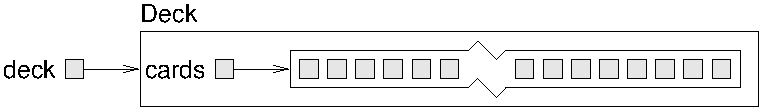
\includegraphics{figs/deckobject.pdf}

Here is a no-argument constructor that makes a
52-card deck and populates it with {\tt Card}s:

\begin{code}
    public Deck() {
        this.cards = new Card[52];
        int index = 0;
        for (int suit = 0; suit <= 3; suit++) {
            for (int rank = 1; rank <= 13; rank++) {
                cards[index] = new Card(suit, rank);
                index++;
            }
        }
    }
\end{code}

This method is similar to {\tt makeDeck};
we just changed the syntax to make it a constructor.
To invoke it, we use {\tt new}:

\index{new}
\index{statement!new}

\begin{code}
    Deck deck = new Deck();
\end{code}

Now it makes sense to put
the methods that pertain to {\tt Deck}s in the {\tt Deck}
class definition.  Looking at the methods we have written so
far, one obvious candidate is {\tt printDeck} (Section~\ref{printdeck}).
Here's how it looks, rewritten to work with a {\tt Deck}:
\index{printDeck}

\begin{code}
    public static void printDeck(Deck deck) {
        for (int i = 0; i < deck.cards.length; i++) {
            Card.printCard(deck.cards[i]);
        }
    }
\end{code}

One change is the type of the parameter,
from {\tt Card[]} to {\tt Deck}.

The second change is that we can no
longer use {\tt deck.length} to get the length of the array, because
{\tt deck} is a {\tt Deck} object now, not an array.  It contains an
array, but it is not an array.  So we have to write
{\tt deck.cards.length} to extract the array from the {\tt Deck}
object and get the length of the array.

For the same reason, we have to use {\tt deck.cards[i]} to access an
element of the array, rather than just {\tt deck[i]}.

The last change
is that the invocation of {\tt printCard} has to say explicitly that
{\tt printCard} is defined in the {\tt Card} class.


\section{Shuffling}
\label{shuffle}
\index{shuffling}

For most card games you need to be able to shuffle the deck;
that is, put the cards in a random order.  In Section~\ref{random}
we saw how to generate random numbers, but it is not obvious how
to use them to shuffle a deck.

One possibility is to model the way humans shuffle, which is usually
by dividing the deck in two and then choosing
alternately from each deck.  Since humans usually don't shuffle
perfectly, after about 7 iterations the order of the deck is pretty
well randomized.  But a computer program would have the annoying
property of doing a perfect shuffle every time, which is not really
very random.  In fact, after 8 perfect shuffles, you would find the
deck back in the order you started in.  For more information, see
\url{http://en.wikipedia.org/wiki/Faro_shuffle}.

A better shuffling algorithm is to traverse the deck one card at a
time, and at each iteration choose two cards and swap them.

Here is an outline of how this algorithm works.  To sketch the
program, I am using a combination of Java statements and English
words that is sometimes called {\bf pseudocode}:  \index{pseudocode}

\begin{code}
    for (int i = 0; i < deck.cards.length; i++) {
        // choose a number between i and deck.cards.length-1
        // swap the ith card and the randomly-chosen card
    }
\end{code}

The nice thing about pseudocode is that it often makes it
clear what methods you are going to need.  In this case, we
need something like {\tt randomInt}, which chooses a random
integer between {\tt low} and {\tt high},
and {\tt swapCards} which takes two indices and switches the
cards at the indicated positions.
\index{random number}
\index{swapCards}
\index{reference}

This process---writing pseudocode first and then writing
methods to make it work---is called {\bf top-down development}
(see \url{http://en.wikipedia.org/wiki/Top-down_and_bottom-up_design}).
\index{program development}


\section{Sorting}
\label{sorting}
\index{sorting}

Now that we have messed up the deck, we need a way to put it back in
order.  There is an algorithm for sorting that is ironically similar
to the algorithm for shuffling.  It's called {\bf selection sort}
because it works by traversing the array repeatedly and selecting the
lowest remaining card each time.
\index{selection sort}

During the first iteration we find the lowest card and swap
it with the card in the 0th position.  During the {\tt i}th, we find the
lowest card to the right of {\tt i} and swap it with the {\tt i}th
card.

Here is pseudocode for selection sort:

\begin{code}
    for (int i = 0; i < deck.cards.length; i++) {
        // find the lowest card at or to the right of i
        // swap the ith card and the lowest card
    }
\end{code}

Again, the pseudocode helps with the design of the {\bf helper
methods}.  In this case we can use {\tt swapCards} again,
so we only need one new one, called {\tt indexLowestCard},
that takes an array of cards and an index where it should
start looking.
\index{helper method}
\index{method!helper}



\section{Subdecks}
\index{subdeck}

How should we represent a hand or some other subset of a full deck?
One possibility is to create a new class called {\tt Hand}, which
might extend {\tt Deck}.  Another possibility, the one I will
demonstrate, is to represent a hand with a {\tt Deck} object with
fewer than 52 cards.

We might want a method, {\tt subdeck}, that takes a Deck
and a range of indices, and that returns a new Deck that
contains the specified subset of the cards:

\begin{code}
public static Deck subdeck(Deck deck, int low, int high) {
    Deck sub = new Deck(high-low+1);

    for (int i = 0; i<sub.cards.length; i++) {
        sub.cards[i] = deck.cards[low+i];
    }
    return sub;
}
\end{code}

The length of the subdeck is {\tt high-low+1} because both the low
card and high card are included.  This sort of computation can be
confusing, and lead to ``off-by-one'' errors.  Drawing a picture is
usually the best way to avoid them.

Because we provide an argument with {\tt new}, the
contructor that gets invoked will be the first one, which only
allocates the array and doesn't allocate any cards.  Inside the
{\tt for} loop, the subdeck gets populated with copies of the
references from the deck.
\index{constructor}
\index{overloading}

The following is a state diagram of a subdeck being created with the
parameters {\tt low=3} and {\tt high=7}.  The result is a hand with 5
cards that are shared with the original deck; i.e. they are aliased.

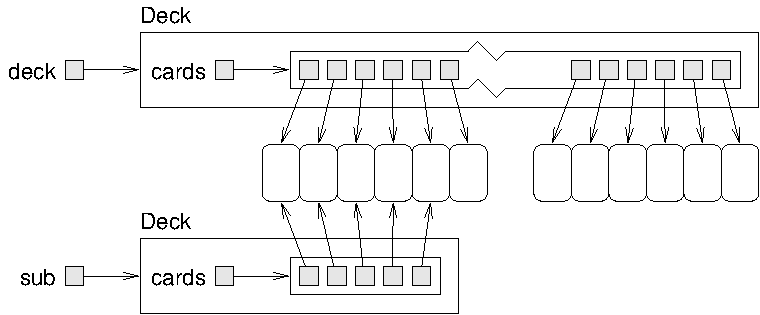
\includegraphics{figs/subdeck.pdf}

\index{aliasing}
\index{reference}

Aliasing is usually not generally a good idea, because
changes in one subdeck are reflected in others, which is not the
behavior you would expect from real cards and decks.  But if the
cards are immutable, aliasing is less dangerous.
In this case, there is probably no reason ever to change the
rank or suit of a card.  Instead we can create each card
once and then treat it as an immutable object.  So for {\tt Card}s
aliasing is a reasonable choice.


\section{Shuffling and dealing}
\index{shuffling}
\index{dealing}

In Section~\ref{shuffle} I wrote pseudocode for a shuffling algorithm.
Assuming that we have a method called {\tt shuffleDeck} that takes
a deck as an argument and shuffles it, we can use it to deal hands:

\begin{code}
    Deck deck = new Deck();
    shuffleDeck(deck);

    Deck hand1 = subdeck(deck, 0, 4);
    Deck hand2 = subdeck(deck, 5, 9);
    Deck pack = subdeck(deck, 10, 51);
\end{code}

This code puts the first 5 cards in one hand, the next 5 cards
in the other, and the rest into the pack.

When you thought about dealing, did you think we should give one
card to each player in the round-robin style that is common
in real card games?  I thought about it, but then realized that it is
unnecessary for a computer program.  The round-robin convention is
intended to mitigate imperfect shuffling and make it more difficult
for the dealer to cheat.  Neither of these is an issue for a computer.

This example is a useful reminder of one of the dangers of engineering
metaphors: sometimes we impose restrictions on computers that are
unnecessary, or expect capabilities that are lacking, because we
unthinkingly extend a metaphor past its breaking point.


\section{Mergesort}
\label{mergesort}
\index{efficiency}
\index{sorting}
\index{mergesort}

In Section~\ref{sorting}, we saw a simple sorting algorithm that turns
out not to be very efficient.  To sort $n$ items, it has to
traverse the array $n$ times, and each traversal takes an amount of
time that is proportional to $n$.  The total time, therefore, is
proportional to $n^2$.

In this section I sketch a more efficient algorithm called {\bf
mergesort}.  To sort $n$ items, mergesort takes time proportional to
$n \log n$.  That may not seem impressive, but as $n$ gets big, the
difference between $n^2$ and $n \log n$ can be enormous.  Try out a
few values of $n$ and see.

The basic idea behind mergesort is this: if you have two subdecks,
each of which has been sorted, it is easy (and fast) to merge them
into a single, sorted deck.  Try this out with a deck of cards:

\begin{enumerate}

\item Form two subdecks with about 10 cards each and sort
them so that when they are face up the lowest cards are on
top.  Place both decks face up in front of you.

\item Compare the top card from each deck and choose the
lower one.  Flip it over and add it to the merged deck.

\item Repeat step two until one of the decks is empty.
Then take the remaining cards and add them to the merged
deck.

\end{enumerate}

The result should be a single sorted deck.  Here's what this
looks like in pseudocode:

\begin{code}
public static Deck merge(Deck d1, Deck d2) {
    // create a new deck big enough for all the cards
    Deck result = new Deck(d1.cards.length + d2.cards.length);

    // use the index i to keep track of where we are in
    // the first deck, and the index j for the second deck
    int i = 0;
    int j = 0;

    // the index k traverses the result deck
    for (int k = 0; k < result.cards.length; k++) {

        // if d1 is empty, d2 wins; if d2 is empty, d1 wins;
        // otherwise, compare the two cards

        // add the winner to the new deck
    }
    return result;
}
\end{code}

The best way to test {\tt merge} is to build and shuffle a deck,
use subdeck to form two (small) hands, and then use the sort
routine from the previous chapter to sort the two halves.  Then
you can pass the two halves to {\tt merge} to see if it works.

\index{testing}

If you can get that working, try a simple implementation of
{\tt mergeSort}:

\begin{code}
public static Deck mergeSort(Deck deck) {
    // find the midpoint of the deck
    // divide the deck into two subdecks
    // sort the subdecks using sortDeck
    // merge the two halves and return the result
}
\end{code}

Then, if you get that working, the real fun begins!  The magical thing
about mergesort is that it is recursive.  At the point where you sort
the subdecks, why should you invoke the old, slow version of {\tt
sort}?  Why not invoke the spiffy new {\tt mergeSort} you are in the
process of writing?
\index{recursion}

Not only is that a good idea, it is {\em necessary} to
achieve the performance advantage I promised.  But to make it
work you have to have a base case; otherwise it recurses
forever.  A simple base case is a subdeck with 0 or 1 cards.  If {\tt
mergesort} receives such a small subdeck, it can return it
unmodified, since it is already sorted.

The recursive version of {\tt mergesort} should look something
like this:

\begin{code}
public static Deck mergeSort(Deck deck) {
    // if the deck is 0 or 1 cards, return it

    // find the midpoint of the deck
    // divide the deck into two subdecks
    // sort the subdecks using mergesort
    // merge the two halves and return the result
}
\end{code}

As usual, there are two ways to think about recursive programs:
you can think through the entire flow of execution, or you
can make the ``leap of faith'' (see Section~\ref{leap of faith}).
I have constructed this example to encourage you to make the leap of faith.
\index{leap of faith}

When you use {\tt sortDeck} to sort the subdecks, you don't
feel compelled to follow the flow of execution, right?  You just
assume it works because you already
debugged it.  Well, all you did to make {\tt mergeSort} recursive was
replace one sorting algorithm with another.  There is no reason to read
the program differently.

Actually, you have to give some thought to getting the
base case right and making sure that you reach it eventually,
but other than that, writing the recursive version should be
no problem.  Good luck!


\section{Class variables}
\index{class variables}

So far we have seen local variables, which are declared inside
a method, and instance variables, which are declared in a class
definition, usually before the method definitions.

Local variables are created when a method is invoked and destroyed
when the method ends.  Instance variables are created when you
create an object and destroyed when the object is garbage collected.

Now it's time to learn about {\bf class variables}.  Like instance
variables, class variables are defined in a class definition before
the method definitions, but they are identified by the keyword {\tt
  static}.  They are created when the program starts and survive until
the program ends.

You can refer to a class variable from anywhere inside the class
definition.  Class variables are often used to store constant
values that are needed in several places.

As an example, here is a version of {\tt Card} where {\tt suits}
and {\tt ranks} are class variables:

\begin{code}
class Card {
    int suit, rank;

    static String[] suits = { "Clubs", "Diamonds", "Hearts", "Spades" };
    static String[] ranks = { "narf", "Ace", "2", "3", "4", "5", "6",
                      "7", "8", "9", "10", "Jack", "Queen", "King" };

    public static void printCard(Card c) {
        System.out.println(ranks[c.rank] + " of " + suits[c.suit]);
    }
}
\end{code}

Inside {\tt printCard} we can refer to {\tt suits} and {\tt ranks} as
if they were local variables.


\section{Glossary}

\begin{description}

\item[pseudocode:]  A way of designing programs by writing
rough drafts in a combination of English and Java.

\item[helper method:]  Often a small method that does not
do anything enormously useful by itself, but which helps
another, more useful method.

\item[class variable:]  A variable declared within a class as {\tt static};
there is always exactly one copy of this variable in existence.

\index{pseudocode}
\index{helper method}
\index{method!helper}
\index{class variables}


\end{description}

\section{Exercises}

\begin{exercise}
The goal of this exercise is to implement the shuffling and
sorting algorithms from this chapter.

\begin{enumerate}

\item Download the code from this chapter from
\url{http://thinkapjava.com/code/Card2.java}
and import it into your development environment.  I have
provided outlines for the methods you will write, so the
program should compile.  But when it runs it prints messages
indicating that the empty methods are not working.  When you
fill them in correctly, the messages should go away.

\item If you did Exercise~\ref{ex.randint}, you already wrote
{\tt randomInt}.  Otherwise, write it now and add code to test it.

\item Write a method called {\tt swapCards} that takes a
deck (array of cards) and two indices, and that switches
the cards at those two locations.

HINT: it should switch references, not
the contents of the objects.  This is faster; also, it
correctly handles the case where cards are aliased.

\item Write a method called {\tt shuffleDeck} that uses the algorithm
in Section~\ref{shuffle}.  You might want to use the {\tt randomInt}
method from Exercise~\ref{ex.randint}.

\item Write a method called {\tt indexLowestCard} that uses
the {\tt compareCard} method to find the lowest card
in a given range of the deck (from {\tt lowIndex} to {\tt highIndex},
including both).

\item Write a method called {\tt sortDeck} that arranges
a deck of cards from lowest to highest.

\item Using the pseudocode in Section~\ref{mergesort}, write the
method called {\tt merge}.  Be sure to test it before trying to use it
as part of a {\tt mergeSort}.

\item Write the simple version of {\tt mergeSort}, the one that
divides the deck in half, uses {\tt sortDeck} to sort the two
halves, and uses {\tt merge} to create a new, fully-sorted deck.

\item Write the fully recursive version of {\tt mergeSort}.
Remember that {\tt sortDeck} is a modifier and {\tt mergeSort} is
a function, which means that they get invoked differently:

\begin{code}
sortDeck(deck);              // modifies existing deck
deck = mergeSort(deck);      // replaces old deck with new
\end{code}

\end{enumerate}
\end{exercise}




%\chapter{Object-oriented programming}
\label{chap13}

\section{Programming languages and styles}
\index{programming language}
\index{language!programming}
\index{programming style}
\index{object-oriented programming}
\index{functional programming}
\index{procedural programming}
\index{programming!object-oriented}
\index{programming!functional}
\index{programming!procedural}

There are many programming languages and almost as many
programming styles (sometimes called paradigms).
The programs we have written so far are {\bf procedural},
because the emphasis has been on specifying computational procedures.

Most Java programs are {\bf object-oriented}, which means that
the focus is on objects and their interactions.
Here are some of the characteristics of object-oriented programming:

\begin{itemize}

\item Objects often represent entities in the real world.
  In the previous chapter, creating the {\tt Deck} class
  was a step toward object-oriented programming.

\item The majority of methods are object methods (like the methods you
  invoke on {\tt Strings}) rather than class methods (like the {\tt Math}
  methods).  The methods we have written so far have
  been class methods.  In this chapter we write some object methods.

\item Objects are isolated from each other by limiting the ways they
  interact, especially by preventing them from accessing
  instance variables without invoking methods.

\item Classes are organized in family trees where
  new classes extend existing classes, adding new methods and
  replacing others.

\end{itemize}

In this chapter I translate the {\tt Card} program from the
previous chapter from procedural to object-oriented style.  You
can download the code from this chapter from
\url{http://thinkapjava.com/code/Card3.java}.


\section{Object methods and class methods}
\index{object method}
\index{method!object}
\index{class method}
\index{method!class}
\index{static}

There are two types of methods in Java, called {\bf class methods} and
{\bf object methods}.  Class methods are identified by the keyword {\tt
  static} in the first line.  Any method that does {\em not} have the
keyword {\tt static} is an object method.

Although we have not written object methods, we have invoked some.
Whenever you invoke a method ``on'' an object, it's an object method.
For example, {\tt charAt} and the other methods we invoked on {\tt String}
objects are all object methods.

For example, here is {\tt printCard} as a class method:

\begin{code}
    public static void printCard(Card c) {
        System.out.println(ranks[c.rank] + " of " + suits[c.suit]);
    }
\end{code}

Anything that can be written as a class method can also be written as an
object method, and vice versa.  But sometimes it is more natural to
use one or the other.
Here it is re-written as an object method:

\begin{code}
    public void print() {
        System.out.println(ranks[rank] + " of " + suits[suit]);
    }
\end{code}

Here are the changes:

\begin{enumerate}

\item I removed {\tt static}.

\item I changed the name of the method to be more idiomatic.

\item I removed the parameter.

\item Inside an object method you can refer to instance variables
as if they were local variables, so I changed {\tt c.rank} to {\tt rank},
and likewise for {\tt suit}.

\end{enumerate}

Here's how this method is invoked:

\begin{code}
    Card card = new Card(1, 1);
    card.print();
\end{code}

When you invoke a method on an object, that object becomes the {\bf
current object}, also known as {\tt this}.  Inside {\tt print},
the keyword {\tt this} refers to the card the method was invoked on.
\index{current object}
\index{object!current}
\index{this}


\section{The {\tt toString} method}
\index{toString}
\index{method!toString}

Every object type has a method called {\tt toString} that returns a
string representation of the object.  When you print an object using
{\tt print} or {\tt println}, Java invokes the object's {\tt toString}
method.

The default
version of {\tt toString} returns a string that contains the type
of the object and a unique identifier (see Section~\ref{printobject}).
When you define a new object
type, you can {\bf override} the default behavior by providing a
new method with the behavior you want.

For example, here is a {\tt toString} method for {\tt Card}:

\begin{code}
public String toString() {
    return ranks[rank] + " of " + suits[suit];
}
\end{code}

The return type is {\tt String}, naturally,
and it takes no parameters.  You can invoke {\tt toString} in
the usual way:

\begin{code}
    Card card = new Card(1, 1);
    String s = card.toString();
\end{code}

or you can invoke it indirectly through {\tt println}:

\begin{code}
    System.out.println(card);
\end{code}


\section{The {\tt equals} method}
\index{equals}
\index{method!equals}

In Section~\ref{equivalence} we talked about two notions of equality:
identity, which means that two variables refer to the same
object, and equivalence, which means that they have the same
value.

The {\tt ==} operator tests identity, but there is no operator
that tests equivalence, because what ``equivalence'' means
depends on the type of the objects.  Instead, objects provide
a method named {\tt equals} that defines equivalence.

Java classes provide {\tt equals} methods that do the right
thing.  But for user defined types the default behavior is the
same as identity, which is usually not what you want.

For {\tt Card}s we already have a method that checks equivalence:

\begin{code}
    public static boolean sameCard(Card c1, Card c2) {
        return (c1.suit == c2.suit && c1.rank == c2.rank);
    }
\end{code}

So all we have to do is rewrite is as an object method:

\begin{code}
    public boolean equals(Card c2) {
        return (suit == c2.suit && rank == c2.rank);
    }
\end{code}

Again, I removed {\tt static} and the first parameter, {\tt c1}.
Here's how it's invoked:

\begin{code}
    Card card = new Card(1, 1);
    Card card2 = new Card(1, 1);
    System.out.println(card.equals(card2));
\end{code}

Inside {\tt equals}, {\tt card} is the current object and {\tt card2}
is the parameter, {\tt c2}.  For methods that operate on two objects
of the same type, I sometimes use {\tt this} explicitly and call
the parameter {\tt that}:

\begin{code}
    public boolean equals(Card that) {
        return (this.suit == that.suit && this.rank == that.rank);
    }
\end{code}

I think it improves readability.


\section{Oddities and errors}
\index{method!object}
\index{method!class}
\index{overloading}

If you have object methods and class methods in the same class, it is
easy to get confused.  A common way to organize a class definition is
to put all the constructors at the beginning, followed by all the
object methods and then all the class methods.

You can have an object method and a class method with the same
name, as long as they do not have the same number and types of
parameters.  As with other kinds of overloading, Java decides
which version to invoke by looking at the arguments you provide.
\index{static}

Now that we know what the keyword {\tt static} means, you
have probably figured out that {\tt main} is a class method,
which means that there is no ``current object'' when it is invoked.
\index{current object}
\index{this}
\index{instance variable}
\index{variable!instance}
%
Since there is no current object in a class method, it is an
error to use the keyword {\tt this}.  If you try, you get
an error message like: ``Undefined variable: this.''

Also, you cannot refer to instance variables without using dot
notation and providing an object name.  If you try, you get a message
like ``non-static variable... cannot be referenced from a static
context.''  By ``non-static variable'' it means ``instance variable.''


\section{Inheritance}
\index{inheritance}

The language feature most often associated with
object-oriented programming is {\bf inheritance}.  Inheritance is the
ability to define a new class that is a modified version of an
existing class.
%
Extending the metaphor, the existing
class is sometimes called the {\bf parent} class and the new
class is called the {\bf child}.

The primary advantage of this feature is that you can add methods
and instance variables without modifying the
parent.  This is particularly useful for Java classes,
since you can't modify them even if you want to.

If you did the GridWorld exercises (Chapters~\ref{gridworld} and
\ref{gridworld2}) you have seen examples of inheritance:

\begin{code}
public class BoxBug extends Bug {
    private int steps;
    private int sideLength;

    public BoxBug(int length) {
        steps = 0;
        sideLength = length;
    }
}
\end{code}

{\tt BoxBug extends Bug} means that {\tt BoxBug} is a new
kind of {\tt Bug} that inherits the methods and instance
variables of {\tt Bug}.  In addition:

\begin{itemize}

\item The child class can have additional instance variables; in
this example, {\tt BoxBug}s have {\tt steps} and {\tt sideLength}.

\item The child can have additional methods; in this example,
{\tt BoxBugs} have an additional constructor that takes an integer
parameter.

\item The child can {\bf override} a method from the parent; in
this example, the child provides {\tt act} (not shown here),
which overrides the {\tt act} method from the parent.

\end{itemize}

If you did the Graphics exercises in Appendix~\ref{graphics}, you
saw another example:

\begin{code}
public class MyCanvas extends Canvas {

    public void paint(Graphics g) {
        g.fillOval(100, 100, 200, 200);
    }
}
\end{code}

{\tt MyCanvas} is a new kind of {\tt Canvas} with no new methods
or instance variables, but it overrides {\tt paint}.

If you didn't do either of those exercises, now is a good time!


\section{The class hierarchy}
\index{class hierarchy}
\index{Object}
\index{parent class}
\index{class!parent}

In Java, all classes extend some other class.  The most basic class is
called {\tt Object}.  It contains no instance variables, but it
provides the methods {\tt equals} and {\tt toString}, among others.

Many classes extend {\tt Object}, including almost all of the classes
we have written and many Java classes, like {\tt java.awt.Rectangle}.
Any class that does not explicitly name a parent inherits from {\tt
  Object} by default.

Some inheritance chains are much longer, though.  For example, {\tt
  javax.swing.JFrame} extends {\tt java.awt.Frame}, which extends {\tt
  Window}, which extends {\tt Container}, which extends {\tt
  Component}, which extends {\tt Object}.  No matter how long the
chain, {\tt Object} is the common ancestor of all classes.

The ``family tree'' of classes is called the class hierarchy.  {\tt Object}
usually appears at the top, with all the ``child'' classes below.  If
you look at the documentation of {\tt JFrame}, for example, you
see the part of the hierarchy that makes up {\tt JFrame}'s pedigree.


\section{Object-oriented design}
\index{object-oriented design}

Inheritance is a powerful feature.  Some programs that would be
complicated without it can be written concisely and simply
with it.  Also, inheritance can facilitate code reuse, since you can
customize the behavior of existing classes without having to modify
them.

On the other hand, inheritance can make programs hard to read.  When
you see a method invocation, it can be hard to figure out which method
gets invoked.

Also, many of the things that can be done with inheritance can
be done as well or better without it.
A common alternative is {\bf composition}, where new objects are
composed of existing objects, adding new capability without
inheritance.

Designing objects and the relationships among them is the topic
of {\bf object-oriented design}, which is beyond the scope of this
book.  But if you are interested, I recommend {\em Head First Design
Patterns}, published by O'Reilly Media.


\section{Glossary}

\begin{description}

\item[object method:]  A method that is invoked on an object,
and that operates on that object.
%, which is referred to by the keyword {\tt this} in Java
% or ``the current object'' in English.
Object methods do not have the keyword {\tt static}.

\item[class method:]  A method with the keyword {\tt static}.
Class methods are not invoked on objects and they do not have
a current object.

\item[current object:]  The object on which an object method
is invoked.  Inside the method,
the current object is referred to by {\tt this}.

%\item[{\tt this}:]  The keyword that refers to the current object.

\item[implicit:]  Anything that is left unsaid or implied.  Within
an object method, you can refer to the instance variables
implicitly (i.e., without naming the object).

\item[explicit:]  Anything that is spelled out completely.  Within
a class method, all references to the instance variables have to
be explicit.

\index{object method}
\index{class method}
\index{current object}
\index{this}
\index{implicit}
\index{explicit}

\end{description}


\section{Exercises}

\begin{exercise}

Download \url{http://thinkapjava.com/code/CardSoln2.java} and
\url{http://thinkapjava.com/code/CardSoln3.java}.

{\tt CardSoln2.java} contains solutions to the exercises
in the previous chapter.  It uses only class methods (except the
constructors).

{\tt CardSoln3.java} contains the same program, but most of the
methods are object methods.  I left {\tt merge} unchanged because
I think it is more readable as a class method.

Transform {\tt merge} into an object method,
and change {\tt mergeSort} accordingly.  Which version of
{\tt merge} do you prefer?

\end{exercise}


\begin{exercise}

Transform the following class method into an object method.

\begin{code}
public static double abs(Complex c) {
    return Math.sqrt(c.real * c.real + c.imag * c.imag);
}
\end{code}
\end{exercise}


\begin{exercise}
Transform the following object method into a class method.

\begin{code}
public boolean equals(Complex b) {
    return(real == b.real && imag == b.imag);
}
\end{code}
\end{exercise}


\begin{exercise}

This exercise is a continuation of Exercise~\ref{ex.rational}.
The purpose is to practice the syntax of object methods and
get familiar with the relevant error messages.

\begin{enumerate}

\item Transform the methods in the {\tt Rational} class
from class methods to object methods, and make the necessary
changes in {\tt main}.

\item Make a few mistakes.  Try invoking class methods as if
they were object methods and vice-versa.  Try to get a sense for
what is legal and what is not, and for the error messages that
you get when you mess up.

\item Think about the pros and cons of
class and object methods.  Which is more concise (usually)?
Which is a more natural way to express computation (or, maybe
more fairly, what kind of computations can be expressed most
naturally using each style)?

\end{enumerate}
\end{exercise}


\begin{exercise}
The goal of this exercise is to write a program that generates random
poker hands and classifies them, so that we can estimate the
probability of the various poker hands.  If you don't play poker, you
can read about it here
\url{http://en.wikipedia.org/wiki/List_of_poker_hands}.

\begin{enumerate}

\item Start with \url{http://thinkapjava.com/code/CardSoln3.java}
and make sure you can compile and run it.

\item Write a definition for a class named {\tt PokerHand}
that extends {\tt Deck}.

\item Write a {\tt Deck} method named {\tt deal} that creates
a PokerHand, transfers cards from the deck to the hand, and returns
the hand.

\item In {\tt main} use {\tt shuffle} and
{\tt deal} to generate and print four {\tt PokerHands} with
five cards each.  Did you get anything good?

\item Write a {\tt PokerHand} method called {\tt hasFlush}
returns a boolean indicating whether the
hand contains a flush.

\item Write a method called {\tt hasThreeKind} that
indicates whether the hand contains
Three of a Kind.

\item Write a loop that generates a few thousand hands and
checks whether they contain a flush or three of a kind.
Estimate the probability of getting one of those hands.
Compare your results to the probabilities at
\url{http://en.wikipedia.org/wiki/List_of_poker_hands}.

\item Write methods that test for the other poker hands.  Some
are easier than others.  You might find it useful to write some
general-purpose helper methods that can be used for more than one
test.

\item In some poker games, players get seven cards each, and
they form a hand with the best five of the seven.  Modify your
program to generate seven-card hands and recompute the probabilities.

\end{enumerate}
\end{exercise}



%\chapter{GridWorld: Part 3}
\label{gridworld3}

If you haven't done the exercises in Chapters~\ref{gridworld} and
\ref{gridworld2}, you should do them before reading this chapter.
As a reminder, you can find the
documentation for the GridWorld classes at
\url{http://www.greenteapress.com/thinkapjava/javadoc/gridworld/}.

Part 3 of the GridWorld Student Manual presents the classes that
make up GridWorld and the interactions among them.  It is an
example of object-oriented design and an opportunity to discuss OO
design issues.

But before you read the Student Manual, there are a few more things
you need to know.


\section{{\tt ArrayList}}

GridWorld uses {\tt java.util.ArrayList}, which is an object similar
to an array.  It is a {\bf collection}, which means that it's an
object that contains other objects.  Java provides other collections
with different capabilities, but to use GridWorld we only need {\tt
  ArrayList}s.

To see an example, download
\url{http://thinkapjava.com/code/BlueBug.java} and
\url{http://thinkapjava.com/code/BlueBugRunner.java}.
A {\tt BlueBug} is a bug that moves at random and looks for rocks.
If it finds a rock, it makes it blue.

Here's how it works.  When {\tt act} is invoked, {\tt BlueBug} gets
its location and a reference to the grid:

\begin{code}
    Location loc = getLocation();
    Grid<Actor> grid = getGrid();
\end{code}

The type in angle-brackets (\verb"<>") is a {\bf type parameter}
that specifies the contents of {\tt grid}.  In other words, {\tt grid}
is not just a {\tt Grid}, it's a {\tt Grid} that contains {\tt Actor}s.

The next step is to get the neighbors of the current location.
{\tt Grid} provides a method that does just that:

\begin{code}
    ArrayList<Actor> neighbors = grid.getNeighbors(loc);
\end{code}

The return value from {\tt getNeighbors} is an {\tt ArrayList}
of {\tt Actors}.  The {\tt size} method returns the length of
the {\tt ArrayList}, and {\tt get} selects an element.  So
we can print the neighbors like this.

\begin{code}
        for (int i = 0; i < neighbors.size(); i++) {
            Actor actor = neighbors.get(i);
            System.out.println(actor);
        }
\end{code}

Traversing an {\tt ArrayList} is such a common operation there's a
special syntax for it: the {\bf for-each loop}.  So we could write:

\begin{code}
        for (Actor actor : neighbors) {
            System.out.println(actor);
        }
\end{code}

We know that the neighbors are {\tt Actors}, but we don't know
what kind: they could be {\tt Bug}s, {\tt Rock}s, etc.
To find the Rocks, we use the {\tt instanceof} operator, which
checks whether an object is an instance of a class.

\begin{code}
        for (Actor actor : neighbors) {
            if (actor instanceof Rock) {
                actor.setColor(Color.blue);
            }
        }
\end{code}

To make all this work, we need to import the classes we use:

\begin{code}
import info.gridworld.actor.Actor;
import info.gridworld.actor.Bug;
import info.gridworld.actor.Rock;
import info.gridworld.grid.Grid;
import info.gridworld.grid.Location;

import java.awt.Color;
import java.util.ArrayList;
\end{code}


\section{Interfaces}
\index{interface}

GridWorld also uses Java {\bf interfaces}, so I want to explain what
they are.  ``Interface'' means different things in different contexts,
but in Java it refers to a specific language feature:
an interface is a class definition where the methods have no bodies.

In a normal class definition, each method has a prototype and a
body (see Section~\ref{documentation}).  A prototype is also called a
{\bf specification} because it specifies the name, parameters, and
return type of the method. The body is called the {\bf implementation}
because it implements the specification.

In a Java interface the methods have no bodies, so it specifies
the methods without implementing them.

For example, {\tt java.awt.Shape} is an interface with prototypes for
{\tt contains}, {\tt intersects}, and several other methods.  {\tt
  java.awt.Rectangle} provides implementations for those methods, so
we say that ``Rectangle implements Shape.''  In fact, the first line
of the {\tt Rectangle} class definition is:

\begin{code}
public class Rectangle extends Rectangle2D implements Shape, Serializable
\end{code}

Rectangle inherits methods from {\tt Rectangle2D} and provides
implementations for the methods in {\tt Shape} and {\tt Serializable}.

In GridWorld the Location class implements the {\tt
  java.lang.Comparable} interface by providing {\tt compareTo}, which
is similar to {\tt compareCards} in Section~\ref{compare}.
%
GridWorld also defines a new interface, {\tt Grid}, that specifies
the methods a {\tt Grid} should provide.  And it includes two
implementations, {\tt BoundedGrid} and {\tt UnboundedGrid}.

The Student Manual uses the abbreviation {\bf API}, which stands for
``application programming interface.''  The API is the set of methods
that are available for you, the application programmer, to use.  See
\url{http://en.wikipedia.org/wiki/Application_programming_interface}.


\section{{\tt public} and {\tt private}}

Remember in Chapter~\ref{chap01} I said I would explain why the {\tt
  main} method has the keyword {\tt public}?  Finally, the time has
come.

{\tt public} means that the method can be invoked from other classes.
The alternative is {\tt private}, which means the method can only
be invoked inside the class where it is defined.

Instance variables can also be {\tt public} or {\tt private}, with
the same result: a private instance variable can be accessed only
inside the class where it is defined.

The primary reason to make methods and instance variables private
is to limit interactions between classes in order to manage
complexity.

For example, the Location class keeps its instance variables private.
It has accessor methods {\tt getRow} and {\tt getCol}, but it provides
no methods that modify the instance variables.  In effect, Location
objects are immutable, which means that they can be shared without
worrying about unexpected behavior due to aliasing.

Making methods private helps keep the API simple.  Classes often
include helper methods that are used to implement other methods, but
making those methods part of the public API might be unnecessary
and error-prone.

Private methods and instance variables are language features
that help programmers ensure {\bf data encapsulation}, which means
that objects in one class are isolated from other classes.


\section{Game of Life}

The mathematician John Conway invented
the ``Game of Life,'' which he called a ``zero-player game''
because no players are needed to choose strategies or make decisions.
After you set up the initial conditions, you watch the game
play itself.  But that turns out to be more interesting than it sounds;
you can read about it at
\url{http://en.wikipedia.org/wiki/Conways_Game_of_Life}.

The goal of this exercise is to implement the Game of Life in
GridWorld.  The game board is the grid, and the pieces are Rocks.

The game proceeds in turns, or {\bf time steps}.  At the beginning
of the time step, each Rock is either ``alive'' or ``dead''.  On the
screen, the color of the Rock indicates its status.
%
The status of each Rock depends on the status of its
{\bf neighbors}.  Each Rock has 8 neighbors, except the Rocks along
the edge of the Grid.  Here are the rules:

\begin{itemize}

\item If a dead Rock has exactly three neighbors, it comes to life!
Otherwise it stays dead.

\item If a live Rock has 2 or 3 neighbors, it survives.  Otherwise it dies.

\end{itemize}

Some consequences of these rules:
If all Rocks are dead, no Rocks come to life.  If you start with a
single live Rock, it dies.  But if you have 4 Rocks in a square, they
keep each other alive, so that's a stable configuration.

Most simple starting configurations either die out quickly or reach a
stable configuration.  But there are a few starting conditions that
display remarkable complexity.  One of those is the r-pentomino: it
starts with only 5 Rocks, runs for 1103 timesteps and ends in a stable
configuration with 116 live Rocks (see
\url{http://www.conwaylife.com/wiki/R-pentomino}).

The following sections are suggestions for implementing Game of Life
in GridWorld.  You can download my solution at
\url{http://thinkapjava.com/code/LifeRunner.java} and
\url{http://thinkapjava.com/code/LifeRock.java}.


\section{{\tt LifeRunner}}

Make a copy of {\tt BugRunner.java} named {\tt LifeRunner.java}
and add methods with the following prototypes:

\begin{code}
    /**
     * Makes a Game of Life grid with an r-pentomino.
     */
    public static void makeLifeWorld(int rows, int cols)

    /**
     * Fills the grid with LifeRocks.
     */
    public static void makeRocks(ActorWorld world)
\end{code}

{\tt makeLifeWorld} should create a Grid of Actors and an ActorWorld,
then invoke {\tt makeRocks}, which should put a {\tt LifeRock} at
every location in the Grid.


\section{{\tt LifeRock}}

Make a copy of {\tt BoxBug.java} named {\tt LifeRock.java}.
{\tt LifeRock} should extend {\tt Rock}.  Add an {\tt act} method
that does nothing.  At this point you should be able to run the
code and see a Grid full of Rocks.

To keep track of the status of the Rocks, you can add a new instance
variable, or you can use the Color of the Rock to indicate status.
Either way, write methods with these prototypes:

\begin{code}
    /**
     * Returns true if the Rock is alive.
     */
    public boolean isAlive()

    /**
     * Makes the Rock alive.
     */
    public void setAlive()

    /**
     * Makes the Rock dead.
     */
    public void setDead()
\end{code}

Write a constructor that invokes {\tt setDead} and confirm that
all Rocks are dead.


\section{Simultaneous updates}

In the Game of Life, all Rocks are updated simultaneously; that is,
each rock checks the status of its neighbors before any Rocks
change their status.  Otherwise the behavior of the system would
depend on the order of the updates.

In order to implement simultaneous updates, I suggest that you write
an {\tt act} method that has two phases: during the first phase,
all Rocks count their neighbors and record the results; during the
second phase, all Rocks update their status.

Here's what my {\tt act} method looks like:

\begin{code}
    /**
     * Check what phase we're in and calls the appropriate method.
     * Moves to the next phase.
     */
    public void act() {
        if (phase == 1) {
            numNeighbors = countLiveNeighbors();
            phase = 2;
        } else {
            updateStatus();
            phase = 1;
        }
    }
\end{code}

{\tt phase} and {\tt numNeighbors} are instance variables.
And here are the prototypes for {\tt countLiveNeighbors} and
{\tt updateStatus}:

\begin{code}
    /**
     * Counts the number of live neighbors.
     */
    public int countLiveNeighbors()

    /**
     * Updates the status of the Rock (live or dead) based on
     * the number of neighbors.
     */
    public void updateStatus()
\end{code}

Start with a simple version of {\tt updateStatus} that changes live
rocks to dead and vice versa.  Now run the program and confirm that
the Rocks change color.  Every two steps in the World correspond to
one timestep in the Game of Life.

Now fill in the bodies of {\tt countLiveNeighbors} and
{\tt updateStatus} according to the rules and see if the system behaves
as expected.


\section{Initial conditions}

To change the initial conditions, you can use the GridWorld pop-up
menus to set the status of the Rocks by invoking {\tt setAlive}.
Or you can write methods to automate the process.

In {\tt LifeRunner}, add a method called {\tt makeRow} that creates
an initial configuration with {\tt n} live Rocks in a row in the middle
of the grid.  What happens for different values of {\tt n}?

Add a method called {\tt makePentomino} that creates
an r-pentomino in the middle of the Grid.  The initial configuration
should look like this:

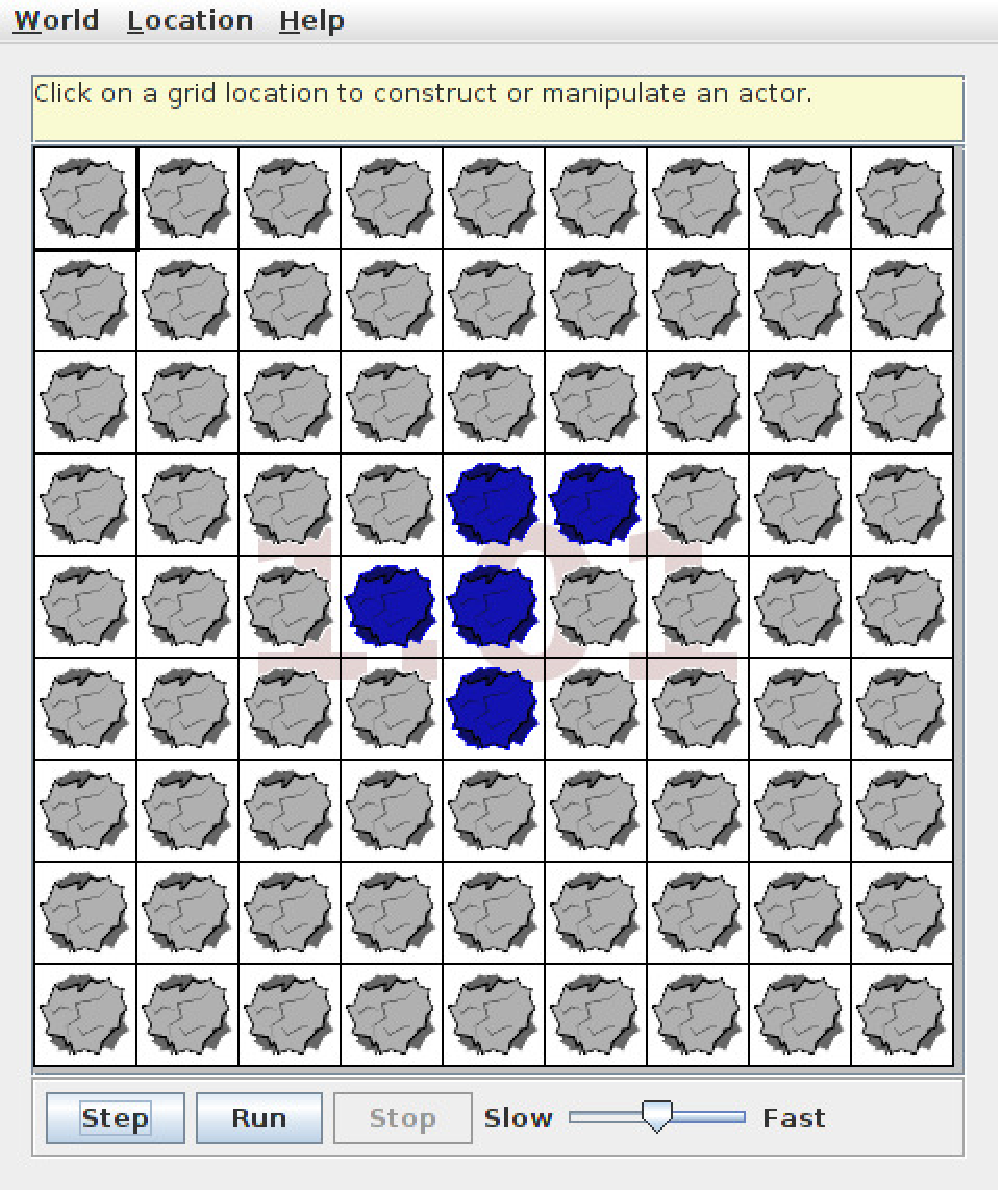
\includegraphics[height=2in]{figs/LifeRunner.pdf}

If you run this configuration for more than a few steps, it reaches the
end of the Grid.  The boundaries of the Grid change the behavior of
the system; in order to see the full evolution of the r-pentomino,
the Grid has to be big enough.  You might have to experiment to find
the right size, and depending on the speed of your computer, it
might take a while.

The Game of Life web page describes other initial conditions that
yield interesting results (\url{http://www.conwaylife.com/}).  Choose
one you like and implement it.

There are also variations of the Game of Life based on different rules.
Try one out and see if you find anything interesting.

\section{Exercises}

\begin{exercise}
Starting with a copy of {\tt BlueBug.java}, write a class definition
for a new kind of {\tt Bug} that finds and eats flowers.  You can
``eat'' a flower by invoking {\tt removeSelfFromGrid} on it.
\end{exercise}

\begin{exercise}
Now you know what you need to know to read Part 3 of the
GridWorld Student Manual and do the exercises.
\end{exercise}

\begin{exercise}
If you implemented the Game of Life, you are well prepared for
Part 4 of the GridWorld Student Manual.  Read it and do the exercises.
\end{exercise}


Congratulations, you're done!


\backmatter
\appendix

%\chapter{Graphics}
\label{graphics}

\section{Java 2D Graphics}
\index{class!Graphics}
\index{Graphics}
\index{class!Frame}
\index{Frame}

This appendix provides examples and exercises that demonstrate Java
graphics.  There are several ways to create graphics in Java; the
simplest is to use {\tt java.awt.Graphics}.
Here is a complete example:

\begin{code}
import java.awt.Canvas;
import java.awt.Graphics;
import javax.swing.JFrame;

public class MyCanvas extends Canvas {

    public static void main(String[] args) {
        // make the frame
        JFrame frame = new JFrame();
        frame.setDefaultCloseOperation(JFrame.EXIT_ON_CLOSE);

        // add the canvas
        Canvas canvas = new MyCanvas();
        canvas.setSize(400, 400);
        frame.getContentPane().add(canvas);

        // show the frame
        frame.pack();
        frame.setVisible(true);
    }

    public void paint(Graphics g) {
        // draw a circle
        g.fillOval(100, 100, 200, 200);
    }
}
\end{code}

You can download this code from
\url{http://thinkapjava.com/code/MyCanvas.java}.

The first lines import the classes we need from {\tt java.awt}
and {\tt javax.swing}.

{\tt MyCanvas} extends {\tt Canvas}, which means that a
{\tt MyCanvas} object is a kind of {\tt Canvas} that provides
methods for drawing graphical objects.

In {\tt main} we

\begin{enumerate}

\item Create a {\tt JFrame}, which is a window that can contain the
  canvas, buttons, menus, and other window components;

\item Create {\tt MyCanvas}, set its width and height, and add it
  to the frame; and

\item Display the frame on the screen.

\end{enumerate}

{\tt paint} is a special method that gets invoked
when {\tt MyCanvas} needs to be drawn.
If you run this code, you should see a black circle on a gray
background.


\section{{\tt Graphics} methods}
\index{method!Graphics}
\index{setColor}
\index{drawOval}

To draw on the Canvas, you invoke methods on the
Graphics object.  The previous example uses {\tt fillOval}.
Other methods include {\tt drawLine}, {\tt drawRect} and more.
You can read the documentation of these methods at
\url{http://download.oracle.com/javase/6/docs/api/java/awt/Graphics.html}.

Here is the prototype for {\tt fillOval}:

\begin{code}
public void fillOval(int x, int y, int width, int height)
\end{code}

The parameters specify
a {\bf bounding box}, which is the rectangle
in which the oval is drawn (as shown in the figure).  The
bounding box itself is not drawn.

\index{bounding box}


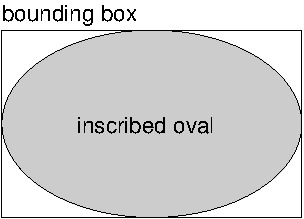
\includegraphics{figs/circle.pdf}

{\tt x} and {\tt y} specify the
the location of the upper-left corner
of the bounding box in the Graphics
{\bf coordinate system}.


\section{Coordinates}
\index{coordinate}
\index{Cartesian coordinate}
\index{graphics coordinate}

You are probably familiar with Cartesian coordinates in two
dimensions, where each location is identified by an x-coordinate
(distance along the x-axis) and a y-coordinate.  By convention,
Cartesian coordinates increase to the right and up, as shown in the
figure.


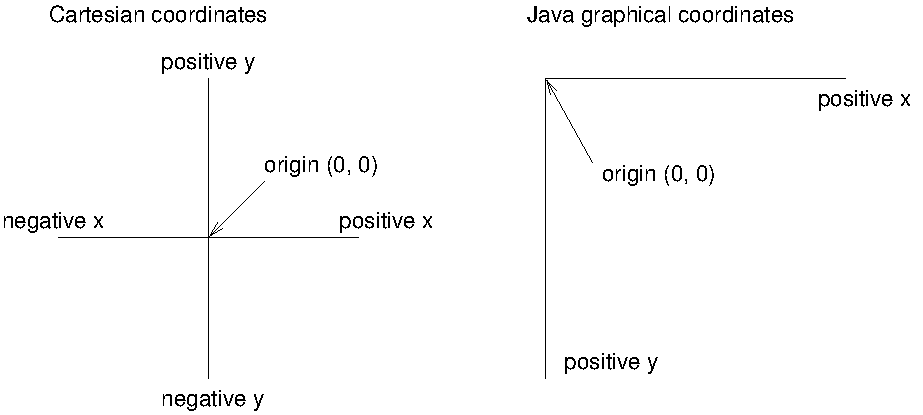
\includegraphics[width=5in]{figs/coordinates.pdf}


By convention, computer graphics systems to use a
coordinate system where the origin is in the
upper-left corner, and the direction of the
positive y-axis is {\em down}.  Java follows this convention.

\index{pixel}

Coordinates are measured in {\bf pixels}; each pixel corresponds to
a dot on the screen.  A typical screen is about
1000 pixels wide.  Coordinates are always integers.  If you want to
use a floating-point value as a coordinate, you have to round it off
(see Section~\ref{rounding}).


\section{Color}

To choose the color of a shape, invoke {\tt setColor} on the Graphics
object:

\begin{code}
    g.setColor(Color.red);
\end{code}

{\tt setColor} changes the current color; everything that gets drawn
is the current color.

{\tt Color.red} is a value provided by the {\tt Color}
class; to use it you have to import {\tt java.awt.Color}.
Other colors include:

\begin{stdout}
black     blue    cyan   darkGray   gray   lightGray
magenta   orange  pink   red        white  yellow
\end{stdout}

You can create other colors by specifying red, green and blue (RGB)
components.
See \url{http://download.oracle.com/javase/6/docs/api/java/awt/Color.html}.

You can control the background color of the {\tt Canvas} by
invoking {\tt Canvas.setBackground}.


\section{Mickey Mouse}
\index{Mickey Mouse}

Let's say we want to draw a picture of Mickey Mouse.  We can use the
oval we just drew as the face, and then add ears.  To make the code
more readable, let's use {\tt Rectangles} to represent bounding boxes.

Here's a method that takes a Rectangle and invokes {\tt fillOval}.

\begin{code}
    public void boxOval(Graphics g, Rectangle bb) {
        g.fillOval(bb.x, bb.y, bb.width, bb.height);
    }
\end{code}

And here's a method that draws Mickey:

\begin{code}
    public void mickey(Graphics g, Rectangle bb) {
        boxOval(g, bb);

        int dx = bb.width/2;
        int dy = bb.height/2;
        Rectangle half = new Rectangle(bb.x, bb.y, dx, dy);

        half.translate(-dx/2, -dy/2);
        boxOval(g, half);

        half.translate(dx*2, 0);
        boxOval(g, half);
    }
\end{code}

The first line draws the face.  The next three lines create
a smaller rectangle for the ears.  We translate the rectangle
up and left for the first ear, then right for the second ear.

The result looks like this:


\includegraphics[height=2in]{figs/mickey.pdf}

You can download this code from
\url{http://thinkapjava.com/code/Mickey.java}.


\section{Glossary}

\begin{description}

\item[coordinate:]  A variable or value that specifies a location
in a two-dimensional graphical window.

\item[pixel:]  The unit in which coordinates are measured.

\item[bounding box:]  A common way to specify the coordinates of
a rectangular area.

\index{coordinate}
\index{pixel}
\index{bounding box}

\end{description}


\section{Exercises}

\begin{exercise}
Draw the flag of Japan, a red circle on white background
that is wider than it is tall.
\end{exercise}


\begin{exercise}
Modify {\tt Mickey.java} to draw ears on the ears, and ears on those
ears, and more ears all the way down until the smallest ears are
only 3 pixels wide.

The result should look like Mickey Moose:

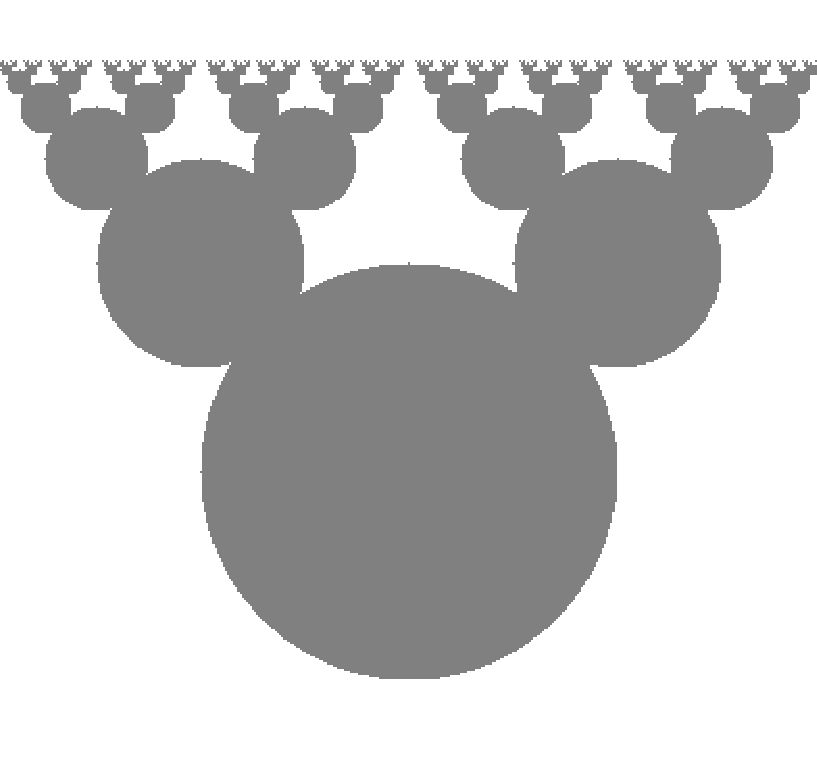
\includegraphics[height=2in]{figs/moose.pdf}

Hint: you should only have to add or modify a few lines of code.

You can download a solution from
\url{http://thinkapjava.com/code/MickeySoln.java}.

\end{exercise}


\begin{exercise}
\begin{enumerate}

\item Download
\url{http://thinkapjava.com/code/Moire.java} and import it into
your development environment.

\item Read the {\tt paint} method and draw a sketch of
what you expect it to do.  Now run it.  Did you get what you
expected?  For an explanation of what is going on, see
\url{http://en.wikipedia.org/wiki/Moire_pattern}.

\item Modify the program so that the space between the circles is
larger or smaller.  See what happens to the image.

\item Modify the program so that the circles are drawn in the center
of the screen and concentric, as in the following figure (left).
The distance between the circles should be small enough
that the Moir\'{e} interference is apparent.

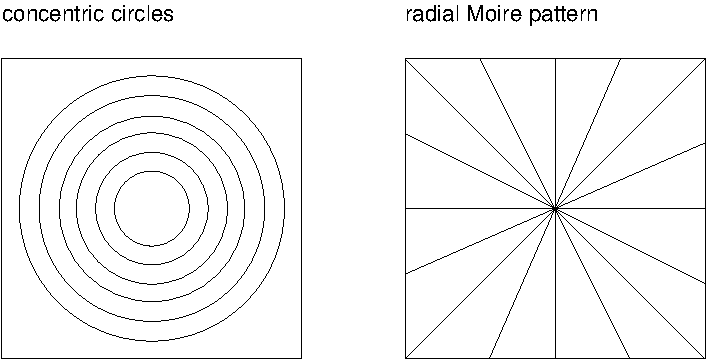
\includegraphics[height=1.5in]{figs/moire.pdf}

\item Write a method named {\tt radial} that draws a radial set
of line segments as shown in the figure (right), but they should be close
enough together to create a Moir\'{e} pattern.

\item Just about any kind of graphical pattern can generate
Moir\'{e}-like interference patterns.  Play around and see what you
can create.

\end{enumerate}
\end{exercise}



%\chapter{Input and Output in Java}
\label{javaio}

\section{Keyboard input}
\label{keyboard}
\index{keyboard}
\index{input!keyboard}

First, you have to use {\tt System.in} to create a new
{\tt InputStreamReader}.

\begin{code}
    InputStreamReader in = new InputStreamReader(System.in);
\end{code}

Then you use {\tt in} to create a new {\tt BufferedReader}:

\begin{code}
    BufferedReader keyboard = new BufferedReader(in);
\end{code}

Finally you can invoke {\tt readLine} on {\tt keyboard},
to take input from the keyboard and convert it to a
String.

\begin{code}
    String s = keyboard.readLine();
    System.out.println(s);
\end{code}

There is only one problem.  There are things that can go wrong when
you invoke {\tt readLine}, and they might throw an {\tt IOException}.  A
method that throws an exception has to include it in the
prototype, like this:

\begin{code}
public static void main(String[] args) throws IOException {
    // body of main
}
\end{code}


\section{File input}
\label{fileIO}
\index{file input}
\index{input!file}

Here's a program that reads lines from a file and prints them:

\begin{code}
import java.io.*;

public class Words {

    public static void main(String[] args)
        throws FileNotFoundException, IOException {

        processFile("words.txt");
    }

    public static void processFile(String filename)
        throws FileNotFoundException, IOException {

        FileReader fileReader = new FileReader(filename);
        BufferedReader in = new BufferedReader(fileReader);

        while (true) {
            String s = in.readLine();
            if (s == null) break;
            System.out.println(s);
        }
    }
}
\end{code}

This first line imports {\tt java.io}, the package that contains
{\tt FileReader}, {\tt BufferedReader}, and the rest of
the elaborate class hierarchy Java uses to do
common, simple things.  The {\tt *} means it imports all classes
in the package.
\index{import statement}
\index{statement!import}

Here's what the same program looks like in Python:

\begin{verbatim}
for word in open('words.txt'):
    print word
\end{verbatim}

I'm not kidding.  That's the whole program, and it does the same thing.

% From Leslie Klein:
% Put the words.txt file directly under your project---not in a package in your project.
% For example, if your project is ThinkJava, then put the words.txt file immediately under ThinkJava.
% Don't put the file in ThinkJava/src/some_package.


\section{Catching exceptions}

In the previous example, {\tt processFile} can throw
{\tt FileNotFoundException} and {\tt IOException}.  And since
{\tt main} calls {\tt processFile}, it has to declare the
same exceptions.  In a larger program, {\tt main} might
declare every exception there is.

The alternative is to {\bf catch} the exception with a
{\tt try} statement.  Here's an example:
\index{try statement}
\index{statement!try}

\begin{code}
    public static void main(String[] args) {
        try {
            processFile("words.txt");
        } catch (Exception ex) {
            System.out.println("That didn't work.  Here's why:");
            ex.printStackTrace();
        }
    }
\end{code}

The structure is similar to an {\tt if} statement.  If the first
``branch'' runs without causing an Exception, the second branch
is skipped.

If the first branch causes an Exception, the flow of execution jumps
to the second branch, which tries to deal with the exceptional
condition (by saying ``error'' in a polite way).  In this case it prints
an error message and the stack trace.

You can download this code from
\url{http://thinkapjava.com/code/Words.java}
and the word list from
\url{http://thinkapjava.com/code/words.txt}.
Make sure both files are in the same folder.
(If you are using an IDE like NetBeans or Eclipse, make
sure the words.txt file is in your project directory.)

Now go do Exercises~\ref{palindrome}, \ref{abecedarian}, and \ref{dupledrome}.




%\chapter{Program development}
\label{development}


% from the end of Section 6.4 Overloading

And that reminds me of one of the cardinal rules of debugging: {\bf make sure that the version of the program you are looking at is the version of the program that is running!}

Some day you may find yourself making one change after another in your program, and seeing the same thing every time you run it.
This is a warning sign that you are not running the version of the program you think you are.
To check, add a {\tt print} statement (it doesn't matter what you print) and make sure the behavior of the program changes accordingly.


\section{Strategies}

I present different program development strategies throughout
the book, so I wanted to pull them together here.
%
The foundation of all strategies is {\bf incremental development},
which goes like this:

\begin{enumerate}

\item Start with a working program that does something visible,
   like printing something.

\item Add a small number of lines of code at a time,
   and test the program after every change.

\item Repeat until the program does what it is supposed to do.

\end{enumerate}

After every change, the program should produce some visible effect
that tests the new code.  This approach to programming can save
a lot of time.

Because you only add a few lines of code at a time, it
is easy to find syntax errors.
%
And because each version of the
program produces a visible result, you are constantly testing your
mental model of how the program works.  If your mental model is
wrong, you are confronted with the conflict (and have a chance
to correct it) before you write a lot of bad code.

The challenge of incremental development is that is it not
easy to figure out a path from the starting place
to a complete and correct program.
%
To help with that, there are several strategies to choose from:

\begin{description}

\item[Encapsulation and generalization:] If you don't know yet how
to divide the computation into methods, start writing code in
{\tt main}, then look for coherent chunks to encapsulate in
a method, and generalize them appropriately.

\item[Rapid prototyping:] If you know what method to write, but not
how to write it, start with a rough draft that handles the simplest
case, then test it with other cases, extending and correcting as you go.

\item[Bottom-up:] Start by writing simple methods, then assemble them
into a solution.

\item[Top-down:] Use pseudocode to design the structure of the
computation and identify the methods you'll need.  Then write the
methods and replace the pseudocode with real code.

\end{description}

Along the way, you might need some scaffolding. For example, each
class should have a {\tt toString} method that lets you print the
state of an object in human-readable form.  This method is useful
for debugging, but usually not part of a finished program.

\section{Failure modes}

If you are spending a lot of time debugging, it is probably
because you are using an ineffective development strategy.  Here
are the failure modes I see most often (and occasionally fall into):

\begin{description}

\item[Non-incremental developement:] If you write more than a few
  lines of code without compiling and testing, you are asking for
  trouble.  One time when I asked a student how the homework was
  coming along, he said, ``Great!  I have it all written.  Now I just
  have to debug it.''

\item[Attachment to bad code:] If you write more than a few lines of
  code without compiling and testing, you may not be able to debug it.
  Ever.  Sometimes the only strategy is (gasp!)~to delete the bad
  code and start over (using an incremental strategy).  But beginners
  are often emotionally attached to their code, even if it doesn't
  work.  The only way out of this trap is to be ruthless.

\item[Random-walk programming:] I sometimes work with students who
  seem to be programming at random.  They make a change, run the
  program, get an error, make a change, run the program, etc.  The
  problem is that there is no apparent connection between the outcome
  of the program and the change.
%
  If you get an error message, take the time to read it.
  More generally, take time to think.

\item[Compiler submission:] Error messages are useful, but they
  are not always right.  For example, if the message says, ``Semi-colon
  expected on line 13,'' that means there is a syntax error near
  line 13. But putting a semi-colon on line 13 is not always the
  solution.  Don't submit to the will of the compiler.

\end{description}

The next chapter makes more suggestions for effective debugging.



%\chapter{Debugging}
\label{debug}
\index{debugging}

The best debugging strategy depends on what kind of error
you have:

\begin{itemize}

\item Syntax errors are produced by the compiler and indicate that
  there is something wrong with the syntax of the program.  Example:
  omitting the semi-colon at the end of a statement.
\index{syntax error}

\item Exceptions are produced if something goes wrong while the
  program is running.  Example: an infinite recursion eventually
  causes a {\tt StackOverflowException}.
\index{exception}
\index{run-time error}

\item Logic errors cause the program to do the wrong thing.  Example:
  an expression may not be evaluated in the order you expect, yielding
  an unexpected result.
\index{logic error}

\end{itemize}

\index{error!syntax}
\index{error!run-time}
\index{error!logic}

The following sections are organized by error type;
some techniques are useful for more than one type.


\section{Syntax errors}

The best kind of debugging is the kind you don't have to do
because you avoid making errors in the first place.  In the
previous section, I suggested development strategies that
minimize errors and makes it easy to find them when you do.
%
The key is to start with a working program and add small
amounts of code at a time.  When there is an error, you will
have a pretty good idea where it is.

Nevertheless, you might find yourself in one of the following
situations.  For each situation, I make some suggestions about
how to proceed.


\subsection*{The compiler is spewing error messages.}
\index{error messages}
\index{compiler}

If the compiler reports 100 error messages, that doesn't mean
there are 100 errors in your program.  When the compiler encounters
an error, it often gets thrown off track for a while.  It tries to
recover and pick up again after the first error, but sometimes
it reports spurious errors.

Only the first error message is truly reliable.  I suggest
that you only fix one error at a time, and then recompile the
program.  You may find that one semi-colon ``fixes'' 100 errors.


\subsection*{I'm getting a weird compiler message and it
won't go away.}

First of all, read the error message carefully.  It is written in
terse jargon, but often there is a carefully hidden kernel of
information.

If nothing else, the message will tell you where in the program the
problem occurred.  Actually, it tells you where the compiler was
when it noticed a problem, which is not necessarily where the error
is.  Use the information the compiler gives you as a guideline,
but if you don't see an error where the compiler is pointing,
broaden the search.

Generally the error will be prior to the location of the error
message, but there are cases where it will be somewhere else
entirely.  For example, if you get an error message at a method
invocation, the actual error may be in the method definition.

If you don't find the error quickly, take a breath and look more
broadly at the entire program.  Make sure the program is indented
properly; that makes it easier to spot syntax errors.

Now, start looking for common errors:
\index{syntax}

\begin{enumerate}

\item Check that all parentheses and brackets are
balanced and properly nested.  All method definitions should be nested
within a class definition.  All program statements should be within a
method definition.

\item Remember that upper case letters are not the same as
lower case letters.

\item Check for semi-colons at the end of statements (and
no semi-colons after squiggly-braces).

\item Make sure that any strings in the code have matching
quotation marks.  Make sure that you use double-quotes for
Strings and single quotes for characters.

\item For each assignment statement, make sure that the type
on the left is the same as the type on the right.  Make sure
that the expression on the left is a variable name or something
else that you can assign a value to (like an element of an array).

\item For each method invocation, make sure that the arguments
you provide are in the right order, and have right type, and that the
object you are invoking the method on is the right type.

\item If you are invoking a value method, make sure you
are doing something with the result.  If you are invoking a
void method, make sure you are {\em not} trying to do something
with the result.

\item If you are invoking an object method, make sure you are
invoking it on an object with the right type.  If you are invoking
a class method from outside the class where it is defined, make
sure you specify the class name.

\item Inside an object method you can refer to the instance
variables without specifying an object.  If you try that in
a class method, you get a message like, ``Static
reference to non-static variable.''

\end{enumerate}

If nothing works, move on to the next section...


\subsection*{I can't get my program to compile no matter
what I do.}

If the compiler says there is an error and you don't see it, that
might be because you and the compiler are not looking at the same
code.  Check your development environment to make sure the program
you are editing is the program the compiler is compiling.  If you
are not sure, try putting an obvious and deliberate syntax error
right at the beginning of the program.  Now compile again.  If
the compiler doesn't find the new error, there is probably something
wrong with the way you set up the development environment.

If you have examined the code thoroughly, and you're sure the compiler
is compiling the right code, it is time for desperate measures:
{\bf debugging by bisection}.
\index{bisection!debugging by}
\index{debugging by bisection}

\begin{itemize}

\item Make a copy of the file you are working on.  If you are
working on {\tt Bob.java}, make a copy called {\tt Bob.java.old}.

\item Delete about half the code from {\tt Bob.java}.  Try compiling
again.

\begin{itemize}

\item If the program compiles now, you know the error is in
the other half.  Bring back about half of the code you deleted and
repeat.

\item If the program still doesn't compile, the error must be in
this half.  Delete about half of the code and repeat.

\end{itemize}

\item Once you have found and fixed the error, start bringing back
the code you deleted, a little bit at a time.

\end{itemize}

This process is ugly, but it goes faster than you might think,
and it is very reliable.


\subsection*{I did what the compiler told me to do, but it
still doesn't work.}

Some compiler messages come with tidbits of advice, like
``class Golfer must be declared
abstract. It does not define int compareTo(java.lang.Object) from
interface java.lang.Comparable.''  It sounds like the compiler
is telling you to declare Golfer as an abstract class, and if
you are reading this book, you probably don't know what that is
or how to do it.

Fortunately, the compiler is wrong.  The solution in this case
is to make sure {\tt Golfer} has a method called {\tt compareTo}
that takes an {\tt Object} as a parameter.

Don't let the compiler lead you by the nose.  Error
messages give you evidence that something is wrong, but
the remedies they suggest are unreliable.


\section{Run-time errors}

\subsection*{My program hangs.}
\index{infinite loop}
\index{infinite recursion}
\index{hanging}

If a program stops and seems to be doing nothing, we
say it is {\bf hanging}.  Often that means that it is caught in
an infinite loop or an infinite recursion.

\begin{itemize}

\item If there is a particular loop that you suspect is the
problem, add a print statement immediately before the loop
that says
``entering the loop'' and another immediately after that
says ``exiting the loop.''

Run the program.  If you get the first message and not
the second, you've got an infinite loop.  Go to the section
titled ``Infinite loop.''

\item Most of the time an infinite recursion will cause the program
to run for a while and then produce a StackOverflowException.
If that happens, go to the section titled ``Infinite recursion.''

If you are not getting a StackOverflowException, but you suspect
there is a problem with a recursive method, you can still use
the techniques in the infinite recursion section.

\item If neither of those suggestions helps, you might not
understand the flow of execution in your program.
Go to the section titled ``Flow of execution.''

\end{itemize}


\subsubsection*{Infinite loop}

If you think you have an infinite loop and you know
which loop it is, add a print statement at
the end of the loop that prints the values of the variables in
the condition, and the value of the condition.

For example,

\begin{code}
    while (x > 0 && y < 0) {
        // do something to x
        // do something to y

        System.out.println("x: " + x);
        System.out.println("y: " + y);
        System.out.println("condition: " + (x > 0 && y < 0));
    }
\end{code}

Now when you run the program you see three lines of output
for each time through the loop.  The last time through the
loop, the condition should be {\tt false}.  If the loop keeps
going, you will see the values of {\tt x} and {\tt y}
and you might figure out why they are not updated correctly.


\subsubsection*{Infinite recursion}

Most of the time an infinite recursion will cause the program
to throw a {\tt StackOverflowException}.  But if the program is
slow it may take a long time to fill the stack.

If you know which method is causing an infinite recursion, check that
there is a base case.  There should be some condition
that makes the method return without making a recursive
invocation.  If not, you need to rethink the algorithm and
identify a base case.

If there is a base case, but the program doesn't seem to be reaching
it, add a print statement at the beginning of the method that prints
the parameters.  Now when you run the program you see a few lines
of output every time the method is invoked, and you see the values of
the parameters.  If the parameters are not moving toward the base case,
you might see why not.


\subsubsection*{Flow of execution}
\index{flow of execution}

If you are not sure how the flow of execution is moving through
your program, add print statements to the beginning of each
method with a message like ``entering method foo,'' where
{\tt foo} is the name of the method.

Now when you run the program it prints a trace of each
method as it is invoked.

You can also print the arguments each method receives.  When you run
the program, check whether the values are reasonable, and check
for one of the most common errors---providing arguments in the wrong
order.


\subsection*{When I run the program I get an Exception.}
\index{Exception}

When an exception occurs, Java prints
a message that includes the name of the
exception, the line of the program where the problem occurred, and a
stack trace.
%
The stack trace includes the method that was running,
the method that invoked it, the method that
invoked {\em that}, and so on.

The first step is to examine the place in the program where
the error occurred and see if you can figure out what happened.

\begin{description}

\item[NullPointerException:] You tried to access an instance
variable or invoke a method on an object that is currently
{\tt null}.  You should figure out which variable is {\tt null}
and then figure out how it got to be that way.

Remember that when you declare a variable with an object type,
it is initially {\tt null} until you assign a value to it.
For example, this code causes a NullPointerException:

\begin{code}
Point blank;
System.out.println(blank.x);
\end{code}

\item[ArrayIndexOutOfBoundsException:] The index you are using
to access an array is either negative or greater than
{\tt array.length-1}.  If you can find the site where the
problem is, add a print statement immediately before it to
print the value of the index and the length of the array.
Is the array the right size?  Is the index the right value?

Now work your way backwards through the program and see where
the array and the index come from.  Find the nearest assignment
statement and see if it is doing the right thing.

If either one is a parameter, go to the place where the method
is invoked and see where the values are coming from.

\item[StackOverFlowException:] See ``Infinite recursion.''

\item[FileNotFoundException:] This means Java didn't find the file
it was looking for.  If you are using a project-based development
environment like Eclipse, you might have to import the file into
the project.  Otherwise make sure the file exists and that the
path is correct.  This problem depends on your file system, so it
can be hard to track down.

\item[ArithmeticException:] Occurs when something goes wrong during
an arithmetic operation, most often division by zero.

\end{description}


\subsection*{I added so many print statements I get inundated with
output.}
\index{print statement}
\index{statement!print}

One of the problems with using print statements for debugging
is that you can end up buried in output.  There are two ways
to proceed: either simplify the output or simplify the program.

To simplify the output, you can remove or comment out print
statements that aren't helping, or combine them, or format
the output so it is easier to understand.  As you develop a program,
you should write code to generate concise,
informative visualizations of what the program is doing.

To simplify the program,
scale down the problem the program is working on.  For example, if you
are sorting an array, sort a {\em small} array.  If the program takes
input from the user, give it the simplest input that causes the
error.

Also, clean up the code.  Remove dead code and reorganize the
program to make it easier to read.  For example, if you
suspect that the error is in a deeply-nested part of the program,
rewrite that part with simpler structure.  If you suspect a
large method, split it into smaller methods and test them
separately.

The process of finding the minimal test case often leads you to the
bug.  For example, if you find that a program works when the array has
an even number of elements, but not when it has an odd number, that
gives you a clue about what is going on.

Reorganizing the program can help you find subtle
bugs.  If you make a change that you think doesn't affect the
program, and it does, that can tip you off.


\section{Logic errors}

\subsection*{My program doesn't work.}

Logic errors are hard to find because the
compiler and the run-time system provide no information about
what is wrong.  Only you know what the program is supposed to
do, and only you know that it isn't doing it.

The first step is to make a connection between the code and the
behavior you get.  You need a hypothesis about what the program
is actually doing.
%
Here are some questions to ask yourself:

\begin{itemize}

\item Is there something the program was supposed to do, but
doesn't seem to be happening?  Find the section of the code
that performs that function and make sure it is executing when
you think it should.  See ``Flow of execution'' above.

\item Is something happening that shouldn't?  Find code in
your program that performs that function and see if it is
executing when it shouldn't.

\item Is a section of code producing an unexpected effect?  Make sure
  you understand the code, especially if it invokes
  Java methods.  Read the documentation for those methods, and
  try them out with simple test cases.  They might not do what you
  think they do.

\end{itemize}

To program, you need a mental model what your code does.
If it doesn't do what you expect, the problem might not be
the program; it might be in your head.
\index{model!mental}
\index{mental model}

The best way to correct your mental model is to break the program
into components (usually the classes and methods) and test
them independently.  Once you find the discrepancy
between your model and reality, you can solve the problem.

Here are some common logic errors to check for:

\begin{itemize}

\item Remember that integer division always rounds down.  If you
want fractions, use {\tt doubles}.

\item Floating-point numbers are only approximate, so don't rely
on perfect accuracy.

\item More generally, use integers for countable things
and floating-point numbers for measurable things.

\item If you use the assignment operator ({\tt =})
instead of the equality operator ({\tt ==}) in the
condition of an {\tt if}, {\tt while}, or {\tt for} statement,
you might get an expression that is syntactically legal and
semantically wrong.

\item When you apply the equality operator ({\tt ==}) to an
object, it checks identity.  If you meant to check
equivalence, you should use the {\tt equals} method.

\item For user defined types, {\tt equals} checks identity.
If you want a different notion of equivalence, you have to
override it.

\item Inheritance can lead to subtle logic errors,
because you can run inherited code without realizing it.
See ``Flow of Execution'' above.

\end{itemize}


\subsection*{I've got a big hairy expression and it doesn't
do what I expect.}
\index{expression!big and hairy}

Writing complex expressions is fine as long as they are readable,
but they can be hard to debug.  It is often a good idea to
break a complex expression into a series of assignments to
temporary variables.

For example:

\begin{code}
rect.setLocation(rect.getLocation().translate(
                -rect.getWidth(), -rect.getHeight()));
\end{code}

Can be rewritten as

\begin{code}
int dx = -rect.getWidth();
int dy = -rect.getHeight();
Point location = rect.getLocation();
Point newLocation = location.translate(dx, dy);
rect.setLocation(newLocation);
\end{code}

The explicit version is easier to read, because the variable
names provide additional documentation, and easier to debug,
because you can check the types of the temporary variables
and display their values.

\index{temporary variable}
\index{variable!temporary}
\index{order of evaluation}
\index{precedence}

Another problem that can occur with big expressions is
that the order of evaluation may not be what you expect.
For example, to evaluate
$\frac{x}{2 \pi}$, you might write

\begin{code}
double y = x / 2 * Math.PI;
\end{code}

That is not correct, because multiplication and division have
the same precedence, and they are evaluated from left to right.
This expression computes $x \pi / 2$.

If you are not sure of the order of operations, use parentheses to
make it explicit.

\begin{code}
double y = x / (2 * Math.PI);
\end{code}

This version is correct,
and more readable for
other people who haven't memorized the order of operations.



\subsection*{My method doesn't return what I expect.}
\index{return statement}
\index{statement!return}

If you have a return statement with a complex expression,
you don't have a chance to print the value before
returning.  Again, you can use a temporary variable.  For
example, instead of

\begin{code}
public Rectangle intersection(Rectangle a, Rectangle b) {
    return new Rectangle(
        Math.min(a.x, b.x),
        Math.min(a.y, b.y),
        Math.max(a.x+a.width, b.x+b.width)-Math.min(a.x, b.x)
        Math.max(a.y+a.height, b.y+b.height)-Math.min(a.y, b.y) );
}
\end{code}

You could write

\begin{code}
public Rectangle intersection(Rectangle a, Rectangle b) {
    int x1 = Math.min(a.x, b.x);
    int y2 = Math.min(a.y, b.y);
    int x2 = Math.max(a.x+a.width, b.x+b.width);
    int y2 = Math.max(a.y+a.height, b.y+b.height);
    Rectangle rect = new Rectangle(x1, y1, x2-x1, y2-y1);
    return rect;
}
\end{code}

Now you have the opportunity to display any of
the intermediate variables before returning.  And by
reusing {\tt x1} and {\tt y1}, you made the code smaller, too.


\subsection*{My print statement isn't doing anything}
\index{print statement}
\index{statement!print}

If you use the {\tt println} method, the output is displayed
immediately, but if you use {\tt print} (at least in some
environments) the output gets stored without being displayed until the
next newline.  If the program terminates without
printing a newline, you may never see the stored output.

If you suspect that this is happening to, change
some or all of the {\tt print} statements to {\tt println}.


\subsection*{I'm really, really stuck and I need help}

First, get away from the computer for a few minutes.
Computers emit waves that affect the brain, causing the following
symptoms:

\begin{itemize}

\item Frustration and rage.

\item Superstitious beliefs (``the computer hates me'') and
magical thinking (``the program only works when I wear my
hat backwards'').

\item Sour grapes (``this program is lame anyway'').

\end{itemize}

If you suffer from any of these symptoms, get
up and go for a walk.  When you are calm, think about the program.
What is it doing?  What are possible causes of that
behavior?  When was the last time you had a working program,
and what did you do next?

Sometimes it just takes time to find a bug.  I often find bugs when I
let my mind wander.  Good places to find bugs are trains, showers, and
bed.


\subsection*{No, I really need help.}

It happens.  Even the best programmers get stuck.
Sometimes you need a fresh pair of eyes.

Before you bring someone else in, make sure you have tried
the techniques described above.  Your program should be as simple
as possible, and you should be working on the smallest input
that causes the error.  You should have print statements in the
appropriate places (and the output they produce should be
comprehensible).  You should understand the problem well enough
to describe it concisely.

When you bring someone in to help, give
them the information they need.

\begin{itemize}

\item What kind of bug is it?  Syntax, run-time, or logic?

\item What was the last thing you did before this error occurred?
What were the last lines of code that you wrote, or what is
the new test case that fails?

\item If the bug occurs at compile-time or run-time, what is
the error message, and what part of the program does it indicate?

\item What have you tried, and what have you learned?

\end{itemize}

By the time you explain the problem
to someone, you might see the answer.  This phenomenon
is so common that some people recommend a debugging technique
called ``rubber ducking.''  Here's how it works:

\begin{enumerate}

\item Buy a standard-issue rubber duck.

\item When you are really stuck on a problem, put the rubber
duck on the desk in front of you and say, ``Rubber duck, I
am stuck on a problem.  Here's what's happening...''

\item Explain the problem to the rubber duck.

\item See the solution.

\item Thank the rubber duck.

\end{enumerate}

I am not kidding.  See
\url{http://en.wikipedia.org/wiki/Rubber_duck_debugging}.


\subsection*{I found the bug!}

When you find the bug, it is usually obvious how to fix it.  But not
always.  Sometimes what seems to be a bug is really an indication that
you don't understand the program, or there is an error in your
algorithm.  In these cases, you might have to rethink the algorithm,
or adjust your mental model.  Take some time away from
the computer to think, work through test cases
by hand, or draw diagrams to represent the computation.

After you fix the bug, don't just start in making new errors.
Take a minute to think about what kind of bug it was, why you made
the error, how the error manifested itself, and
what you could have done to find it faster.  Next time you see something
similar, you will be able to find the bug more quickly.




\printindex
\cleardoublepage

\end{document}
